% openany makes chapters start on even pages too
\documentclass[openany, 12pt]{book}

% sets margins of text inside page to 1 inch
\usepackage[top=1in, bottom=1in, left=1in, right=1in]{geometry}

% this will indent the first paragraph in a chapter
\usepackage{indentfirst}

% to use href
\usepackage{hyperref}

% to use images
\usepackage{graphicx}
% where images are stored
\graphicspath{{src/images/}}

% to use \FloatBarrier
\usepackage[section]{placeins}

\title{
  Introduction to Fitness \\
  \vskip 0.5cm
  \small A Technical Book on Fitness}
\author{Mihail Dunaev}
% this will remove date
\date{}

\begin{document}
  \maketitle
  \tableofcontents

  \chapter{Introduction}
  
	I have no background in fitness or nutrition. In school I studied Computer Science and now I work as a Software Engineer. What made me get more 
	into fitness was my weight: I was fat. Multiple times in my life. First, growing up as a kid I was fat and I managed to lose the weight in 
	secondary school just by eating less. Second time I got fat was in university, just because I lacked any motivation to study for exams and would
	power my way through with food and energy drinks. After uni I found it much harder to lose weight than I previously knew. I would follow a lot  of diets (keto
        \footnote{\href{https://en.wikipedia.org/wiki/Ketogenic_diet}{Ketogenic diet on Wikipedia}}, food replacement like soylent
        \footnote{\href{https://en.wikipedia.org/wiki/Soylent_(meal_replacement)}{Soylent on Wikipedia}} or huel
        \footnote{\href{https://en.wikipedia.org/wiki/Huel}{Huel on Wikipedia}}), sometimes going really low in calories intake, feeling like I 
	have no energy and gaining the weight back on after ending the diet. I needed a better solution to this: I decided to start going to the gym.
	
	I guess my goal was to build muscle and lose fat. I've always liked muscles as a kid, just never got the time to look into it and start
	working out. This was my chance. I had a lot of questions: how do I train? What do I eat? Are there other things I need to pay attention to?
	One solution would be to hire a personal trainer to help me achieve this goal. What stopped me from doing this is the way my brain works: I knew
	I would just be given a list of things to do without any explanation. I really like to understand how things work and I would end up being 
	disappointed. This is also a big part of my life by now, I definitely wanted to understand well how everything works. I started looking into fitness
	the same way I look into everything: start searching on google, looking at professional bodybuilders, what they say, does it make sense etc. 
	I feel that if you want to know a subject really well you should look for competitions related to that subject, and see what the people involved
	have to say about it. This is why I started following people that compete in bodybuilding shows, strongman competitions and so on. 	
	What bothered me was how poorly organised the fitness information I found was. I couldn't find a single place that could take me from 0 knowledge
	to getting started in a matter of few hours. I had to watch a lot of youtube videos, read a lot of articles and posts in fitness communities until
	things were clear in my head. Now that I know all this information I think it's possible to put it all in one place: this is the purpose of this 
	book, to get you started with your fitness journey, especially if your goal is to build muscles and lose fat. And as I understand, this is the case
	for	most people working out.
	
	I just want to stress out: there is nothing wrong with being fat. If you get really fat it is unhealthy and you'll end up with 
	health problems. However, the main reason I don't want to be fat is because I get anxiety from it. I feel like crap, especially if I take my shirt 
	off in public. Saying I don't care about it is just lying to myself and I try my best to not do that, just for my mental health. This anxiety is
	something I can't control so for me the only solution would be to stay in shape. Besides, I already said I like muscles, so becoming muscular would
	make me feel proud of myself.
	
	The book is structured in two parts: nutrition \& workout. There is a lot of information in here, you don't necessarily need to understand all of it
	to get going. That's why at the end, in the last chapter, I just added an example of everything I did to get in my current shape without extra explanations. I will try 
	my best to present information in an unbiased way, presenting what people think works and what not, what I tried on myself etc. If you think 
	something is wrong or don't agree with some of the information presented here, this is an open source book so feel free to submit a PR!
        \footnote{\href{https://docs.github.com/en/free-pro-team@latest/github/collaborating-with-issues-and-pull-requests/about-pull-requests}
	{About pull requests on Github docs}} At the end of the day I am a practical person, I only believe in results and what works in real life. 
	I can say that the information I describe in this book worked really well on me, as you can see in the picture below.
	
	\begin{figure}[h]
		\centering
		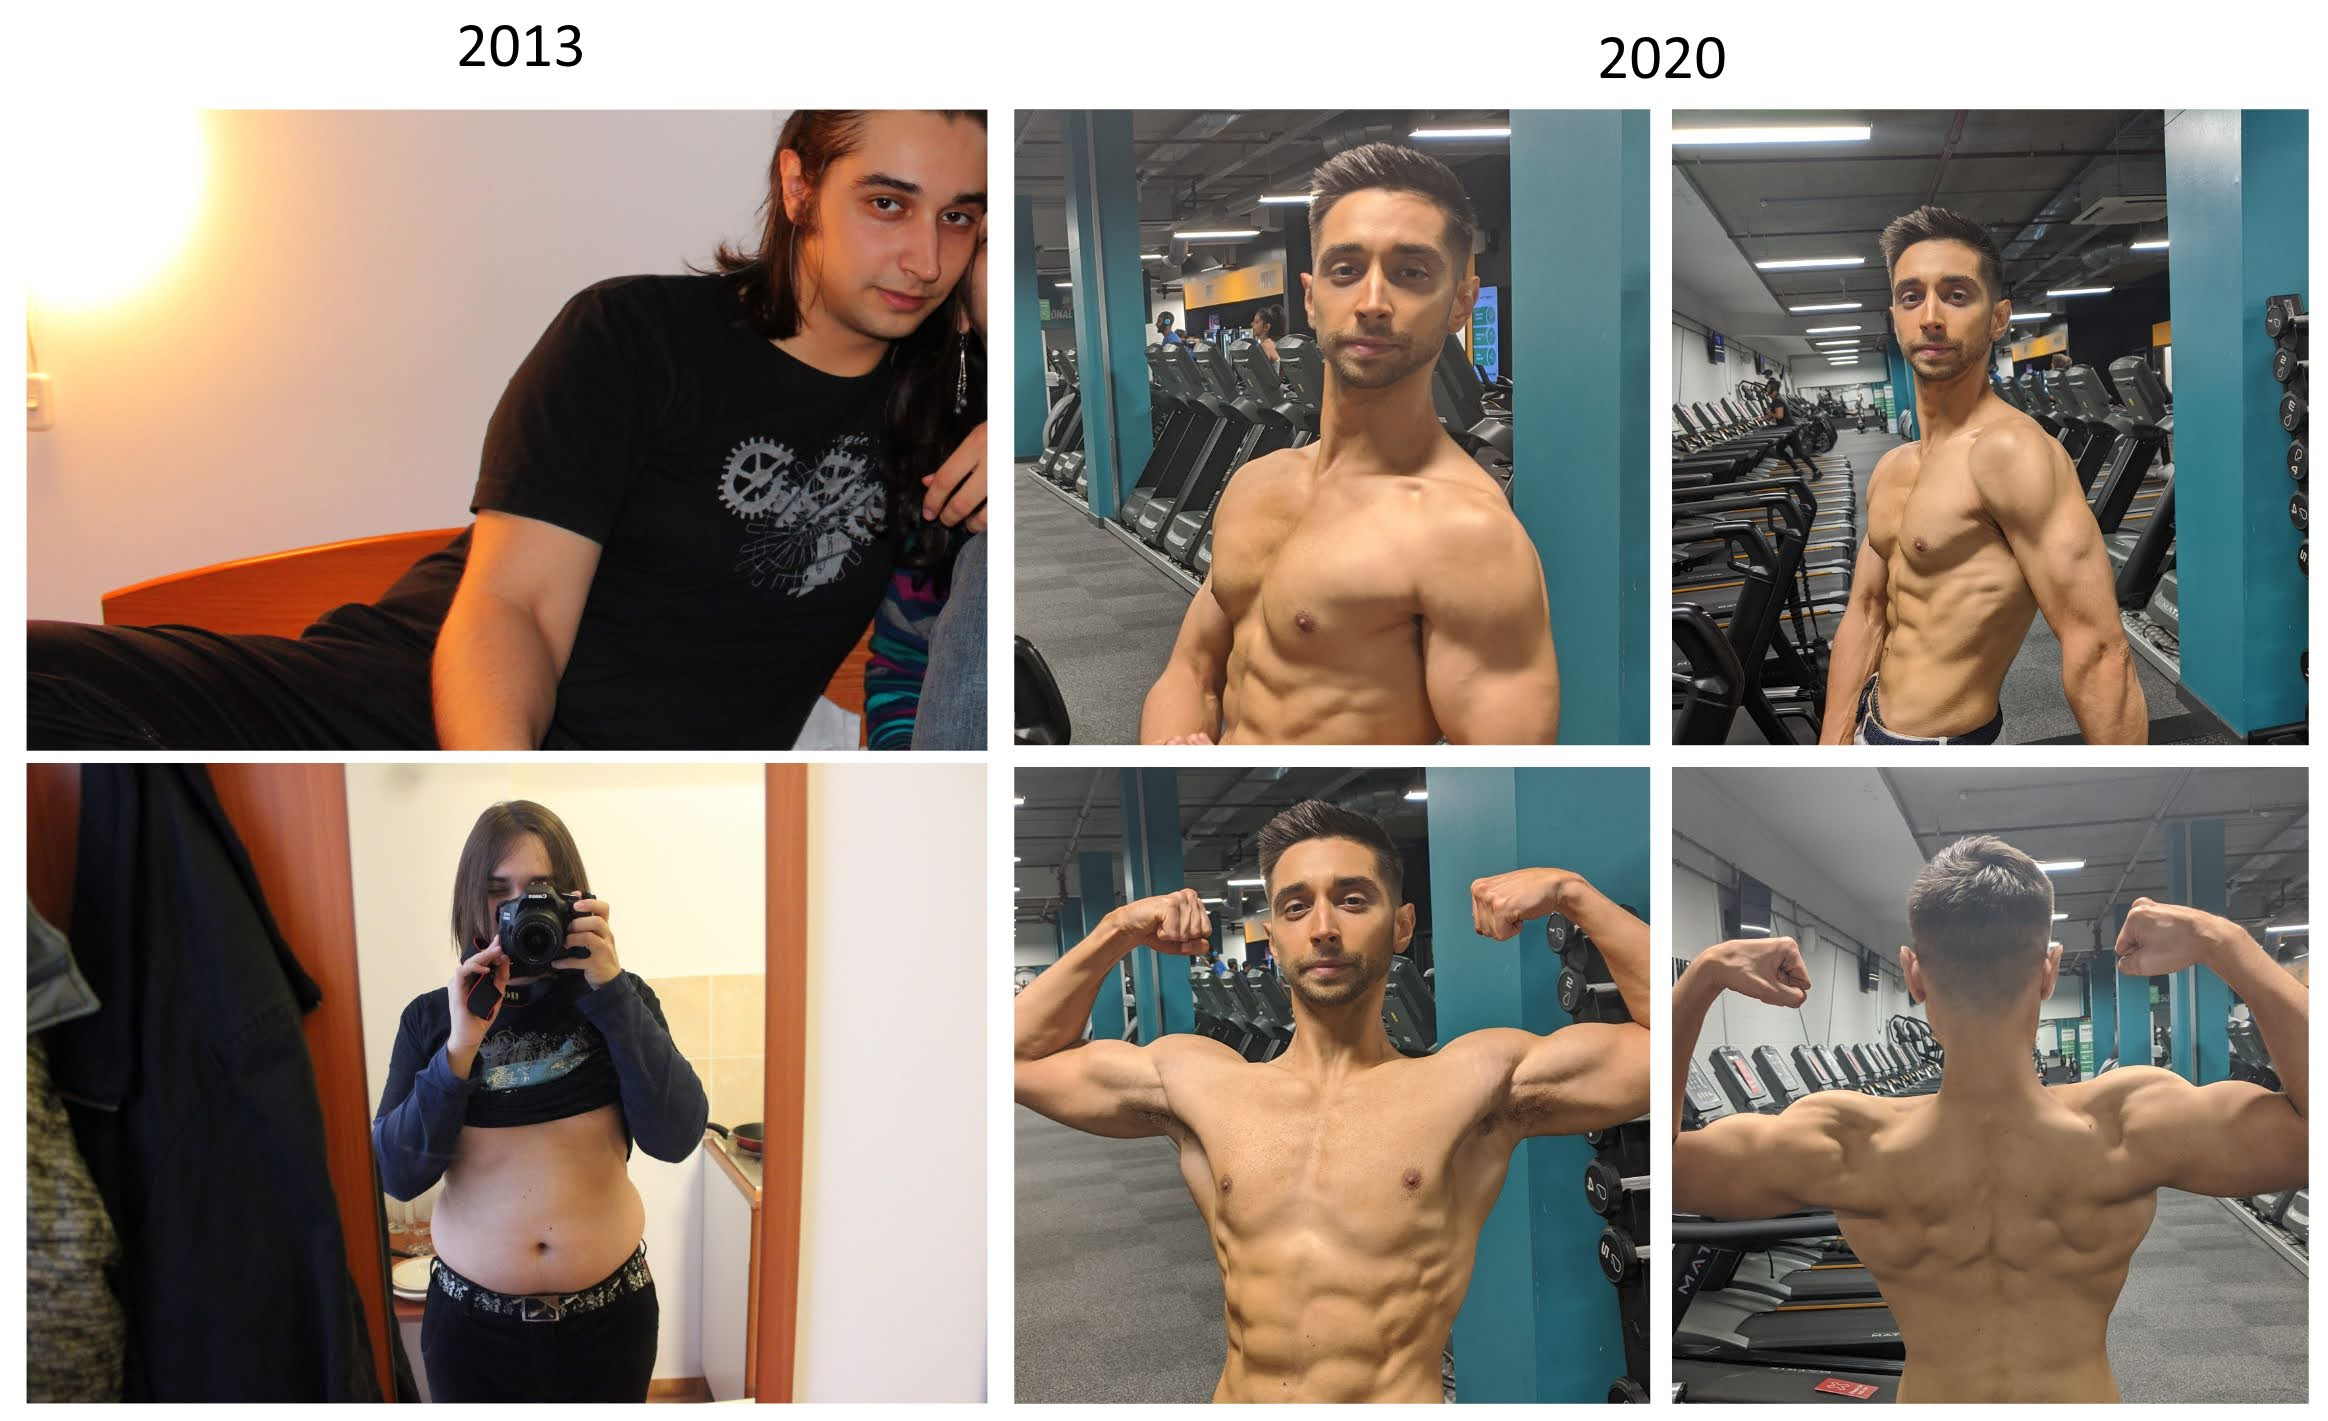
\includegraphics[scale=0.2]{transformation.jpg}
		\caption{From fat to muscular in 7 years: my lifelong struggle with being fat}
		\label{fig1}
	\end{figure}
	
	
  \chapter{Nutrition}
  
  	\section{Calories, BMR, TDEE}
  	
	I feel like I need to explain how food works first before anything else. Your body is an energy converter. It gets energy from food
        \footnote{\href{https://en.wikipedia.org/wiki/Food_energy}{Food energy on Wikipedia}} and converts it to heat, movement (kinetic energy) and 
	electrical energy for thinking. The amount of energy needed without movement (so for heat, thinking and perhaps others things too) is referred 
	to as basal metabolic rate or BMR
        \footnote{\href{https://en.wikipedia.org/wiki/Basal_metabolic_rate}{Basal metabolic rate on Wikipedia}} and it
	doesn't change much from day to day. If you include the energy for movement too you get your total daily energy expenditure or TDEE. If you eat
	more than your TDEE in a day, the extra food will be stored on your body either as fat or muscle. If you eat less then your body will have to go
	to fat stores and muscles and break them down to get the extra food energy you need. Energy is measured in $kcal$, but most of the time you will
	only see the term calorie with the same meaning (basically $kcal$ is the scientific term which was replaced by calorie when it started being used
	by food industries). To put energy values into perspective, the average human would need 2,000 calories for heat every day, or so I've seen in a
	physics course a long time ago. If I run on the treadmill for 1h I get a message that I burned roughly 600 calories. 1 Big Mac has almost 600 calories.
        It's important to understand that knowing exactly how many calories a meal has is next to impossible. There will always be small differences in every
        ingredient you use. For example not all loafs of bread are the same size, not all strawberries contain the same amount of sugar and so on. It's also
        impossible to know exactly how much energy you burn in a day. However, estimates work really well in practice. As long as you eat the same meals every week,
        you will either lose, gain or maintain weight.
	
	People have tried to come up with formulas to compute BMR from different factors, such as height, age, sex or body fat percentage (this is just
	the proportion of fat you have in your body relative to your whole mass, so 100 $\times$ fat mass / body mass). At first only mass (m), height (h) 
	and age (a) were taken into account in Harris-Benedict formula for BMR from 1919
        \footnote{\href{https://en.wikipedia.org/wiki/Harris\%E2\%80\%93Benedict_equation}{Harris-Benedict on Wikipedia}}
	\begin{equation}
		BMR = 13.7516m + 5.0033h - 6.755a + 66.4730
	\end{equation}
  	This formula was later revised in 1984 with just a few minor changes. Later in 1990 Mifflin St Jeor
        \footnote{\href{https://pubmed.ncbi.nlm.nih.gov/2305711/}{A new predictive equation for resting energy expenditure in healthy individuals (1990)}}
        came with 2 formulas for BMR, one for men (\ref{males}) and one for women (\ref{females}).
	\begin{equation}
		\label{males}
		BMR (males) = 10m + 6.25h - 5a + 5
	\end{equation}
	\begin{equation}
		\label{females}
		BMR (females) = 10m + 6.25h - 5a - 161
	\end{equation}
	Finally Katch-McArdle
        \footnote{\href{https://books.google.co.uk/books/about/Essentials_of_Exercise_Physiology.html?id=L4aZIDbmV3oC}{Essentials of Exercise Physiology Book by Katch \& McArdle (2006)}}
        included body fat percentage (f) into the equation, removing age and height
	\begin{equation}
		BMR = 370 + (21.6m (1 - \frac{f}{100}))
	\end{equation}
	This is an interesting point because body fat percentage does affect how many calories you burn even at rest. The rule I know is that 10 pounds of muscle would burn 50 kcal in a day at rest,
        while 10 pounds of fat will only burn 20 kcal
        \footnote{\href{https://www.webmd.com/diet/obesity/features/8-ways-to-burn-calories-and-fight-fat}{Burning calories on WebMD}} (less than half),
        so if you're 80kg with 15\% body fat you will burn more calories at rest than someone who is 80kg with 20\% body fat. This also explains the Mifflin St Jeor above, since women have naturally
        more fat than men.
	
	Let's take an example using the last formula: if you weight $70kg$ and your body fat percentage is $18\%$ then your BMR should be $370 + (21.6 \times 70 \times (1 - 18/100)) = 1609.84$ calories.
        Add your movement energy to this and you get your TDEE. I haven't spent the time trying to derive how to
	compute this one (e.g. from kinetic energy) because all of these formulas are great but at the end of the day they are just for your orientation.
	The best way to compute your TDEE is to actually measure it: without changing your habits, eat 2,000 calories every day for 1-2 weeks. Weight
	yourself every day: does your weight change? If no then it's safe to assume your TDEE is 2,000 calories. Does your weight go up? It probably means
	your TDEE is lower. Keep adjusting your calories intake until you find your TDEE. 
	
	In theory you should be able to tell your TDEE without having
	to change your diet again just by looking at how much weight you gained / lost in the initial 1-2 weeks: you should lose 1lb (or 0.45kg) of mass at 
	a total deficit of 3500 calories
        \footnote{\href{https://www.ncbi.nlm.nih.gov/pmc/articles/PMC2376744/}{What is the required energy deficit per 
	unit weight loss? (2008)}}. Let's take an example again: you ate 2,000 calories for 2 weeks. During these 2 weeks you gained 2.2lbs (or 1kg) on the
	scale. According to the 3500 rule, you were at a total surplus of $3500 \times 2.2 = 7700$ calories. This surplus was achieved in 14 days, so the
	surplus each day was 550 calories. This means your actual TDEE is 2,550 calories. However I found this rule to not work on me, trying to adjust 
	accordingly didn't put me at maintenance and I kept changing weight. As long as you always adjust to results you will be fine. I would personally
	start with an online TDEE calculator
        \footnote{\href{https://tdeecalculator.net/}{Example of online TDEE calculator}} (there are plenty out there) 
	just to get a value to work with, then keep adjusting intake until I hit my maintenance.
	
	\section{Body Fat Percentage}
	
	Body fat percentage is discussed a lot in fitness because it affects how you look. Fat is something that is stored on your body between skin and muscles.
        The more fat you have on you the less visible your muscles will be. However, just taking the absolute value of fat mass is not a good indicator of how well
        your muscles are showing, since taller people will have more fat mass but more body surface to spread it across. So instead we can look at the proportion of
        fat in relation to muscles. The body fat percentage will normally dictate certain features you can see on your body, for example the average guy will have his
        abdominal muscles (``abs'') showing around 10-14\% body fat
        \footnote{\href{https://www.healthline.com/health/body-fat-percentage-for-abs}{Healthline article on abs}}.
        To better understand what I'm talking about look at Figure \ref{bodyfat}. I think it gives a good indication to what body fat percentage looks like at different values.
        In all the pictures I have roughly the same amount of muscles, but different body fat \%. My estimation is, starting with the row at the top: 25.9\%, 19.6\%, 16.5\% and 13\%.
        Usually people say that an ideal body fat \% (both in terms of health and looks) is around 12\% for men
        and around 24\% for women. Another thing to keep in mind is that your genetics will influence how low in body fat \% you can get. For some men reaching 5\% might be
        impossible without taking steroids for example. Also going under 10\% is usually not considered healthy anymore, a lot of people complain about mood, sleep and even sex
        drive problems once you are that low in body fat \%
        \footnote{\href{https://www.youtube.com/watch?v=IHvmtvzOfDg}{VitruvianPhysique on optimal body fat \% on Youtube}}. 
        
	\begin{figure}[h]
		\centering
		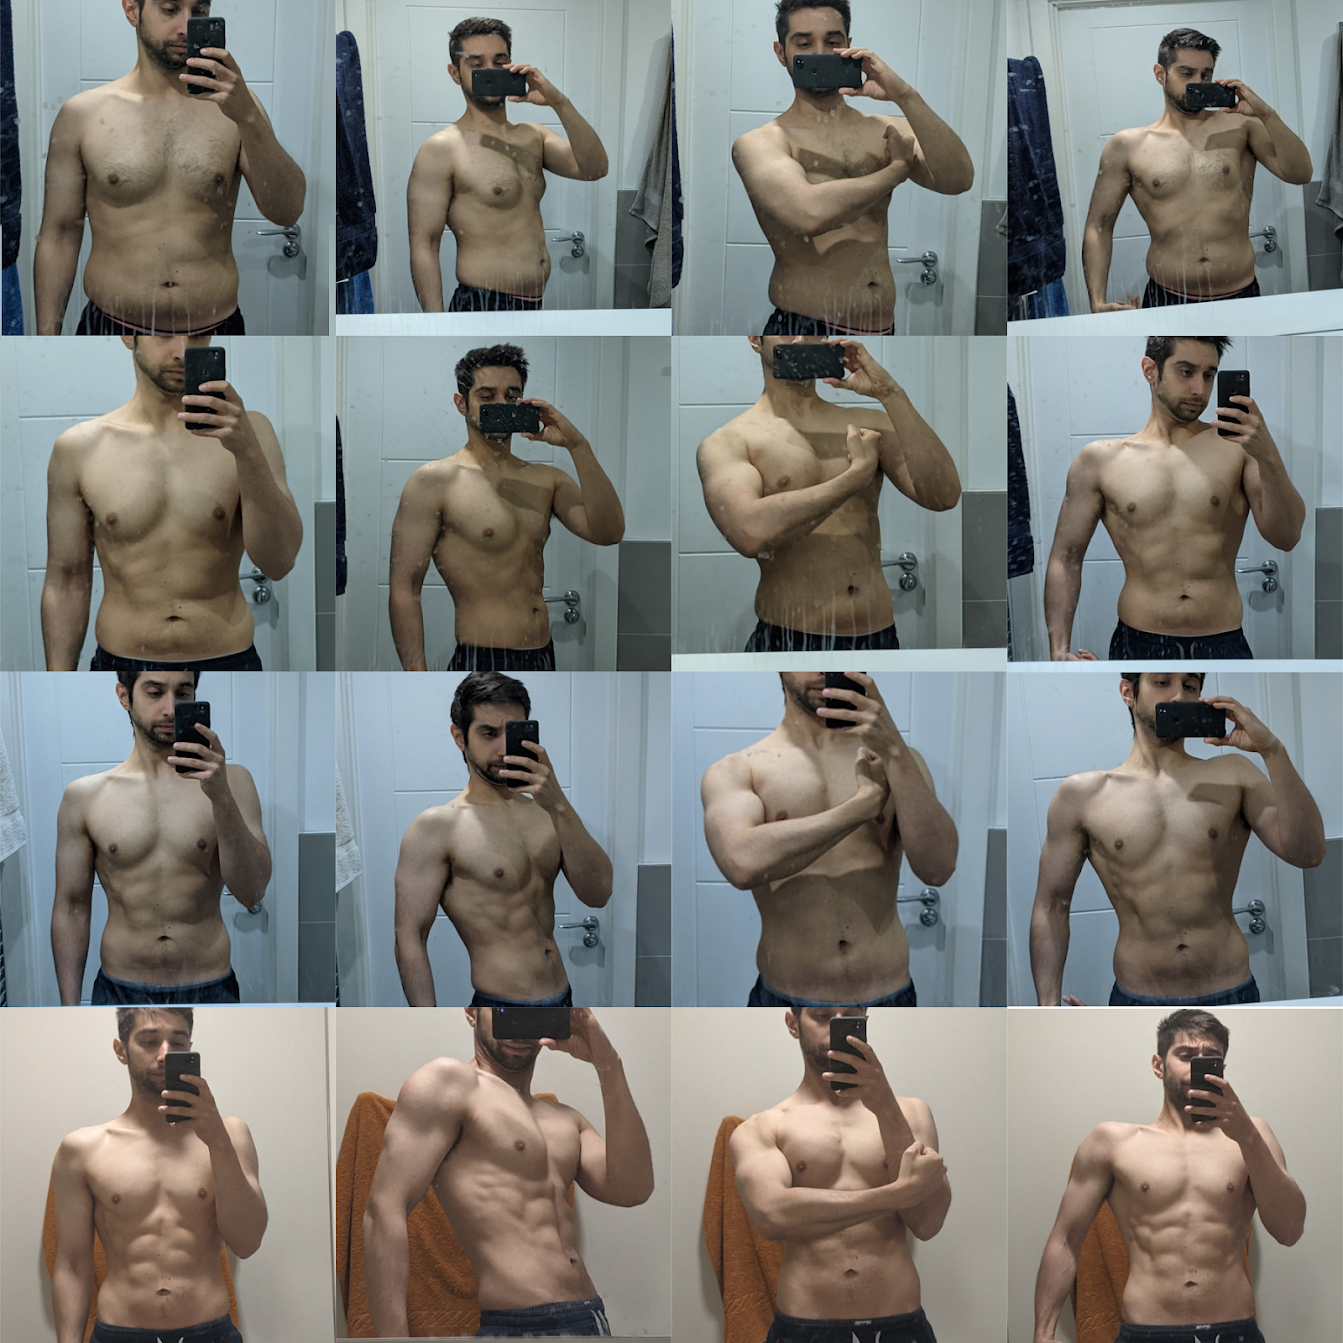
\includegraphics[scale=0.33]{progress-matrix.png}
		\caption{Example of different body fat \% values. Each row has the same body shots at different body fat \%. My estimations from top to bottom: 25.9\%, 19.6\%, 16.5\% and 13\%.
                The muscle mass is roughly the same in every picture, but you can't see it in the first rows because it's covered by fat.}
                \label{bodyfat}
	\end{figure}
	
	Computing body fat percentage is not easy. There is no 100\% accurate way of doing it. You can take pictures of yourself in the mirror and then compare with the images above,
        a lot of people estimate this way and I find it good as well. If you want a more accurate way of doing it though, there are a few options out there. The most accurate way is an MRI scan
        \footnote{\href{https://pubmed.ncbi.nlm.nih.gov/9655763/}{Cadaver validation of skeletal muscle measurement by magnetic resonance imaging and computerized tomography}}.
        However this is not available to the public as far as I know. This leaves us with the second most accurate option I know, which is a DEXA scan
        \footnote{\href{https://en.wikipedia.org/wiki/Dual-energy_X-ray_absorptiometry}{DEXA on Wikipedia}}. This is a machine that does an x-ray scan of your body. It shows quite some details,
        for example the lean mass and fat mass in your arms, trunk (core) and legs. You can see an example of a DEXA scan result in Figure \ref{dexa}.
        However, DEXA scans can have errors too, and a lot of people talk against it
        \footnote{\href{https://www.youtube.com/watch?v=2Gg4Jm5KS1Y}{Greg Doucette on DEXA scans on Youtube}}
        \footnote{\href{https://www.youtube.com/watch?v=P17bcpYE8Ew}{Brain Shaw on DEXA scans on Youtube}}. The scan is also expensive, I did it in London at bodyscan for roughly \pounds 100.
	Before DEXA scans, hydrostatic weighing
        \footnote{\href{https://en.wikipedia.org/wiki/Hydrostatic_weighing}{Hydrostatic weighing on Wikipedia}} was considered the most accurate method
        available to the public. You had to step on a scale underwater and the value you get helps estimate your body density, which can be used to approximate your body fat percentage.
        Another way of estimating body fat percentage which is similar to hydrostatic weighing is whole-body air displacement plethysmography
        \footnote{\href{https://en.wikipedia.org/wiki/Air_displacement_plethysmography}{Air displacement plethysmography on Wikipedia}} (for example Bod Pod
        \footnote{\href{https://www.cosmed.com/en/products/body-composition/bod-pod}{Bod pod}}).
        
	\begin{figure}[h]
		\centering
		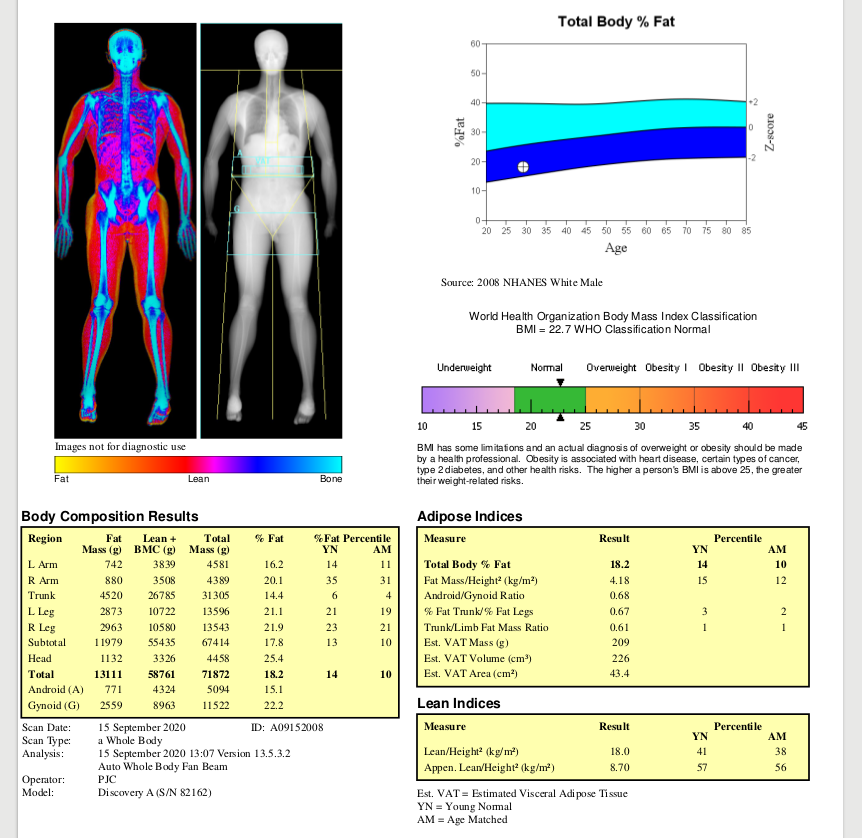
\includegraphics[scale=0.6]{dexa-scan.png}
		\caption{Result of a DEXA scan, showing body fat for different body parts}
                \label{dexa}
	\end{figure}
	
	More common methods of estimating body fat are the skinfold methods
        \footnote{\href{https://en.wikipedia.org/wiki/Body_fat_percentage\#Anthropometric_methods}{Skinfold methods on Wikipedia}}
        (using a device called caliper) and using bioelectrical impedance analysis
        \footnote{\href{https://en.wikipedia.org/wiki/Bioelectrical_impedance_analysis}{Bioelectrical impedance analysis on Wikipedia}}.
        The first method tries to determine the thickness of the fat layer under the skin. You use the caliper at various spots on the body and look up the measurement in
        a table which will tell you the estimated body fat. It's best if you use a personal trainer or someone with experience to perform the reading. For bioelectrical impedance analysis a small
        electric current is sent through the body and the resistance of the whole body is computed, which depends on body fat percentage. Some scales also state they can compute body fat percentage
        just from your weight, height, age and sex. However this is not really possible unless you don't train at all and the extra weight comes from fat alone. Just to recap all the methods
        described in this section, from most accurate to least one:
	
	\begin{enumerate}
		\item Magnetic Resonance Imaging (MRI) and Computerized Tomography (CT)
		\item Dual-energy X-ray absorptiometry (DEXA / DXA)
		\item Hydrostatic weighing
		\item Whole-body air displacement plethysmography
		\item Skinfold methods (calipers)
		\item Bioelectrical impedance analysis
	\end{enumerate}
	
	\section{Macronutrients}
	
	The food you eat can be broken down into different components. The stuff that gives you energy (e.g. for movement) is called macronutrients --- these are carbohydrates
	(carbs), fat \& protein. The stuff that doesn't give you energy is called micronutrients (e.g. vitamins \& minerals). You still need micronutrients to be a healthy individual.
	The reason people talk so much about macronutrients (or macros) is because your body process them differently: carbs can be broken down and used for energy faster than fats,
	proteins are the only macros that can be stored as muscle on your body and so on. It's hard for you to tell how many carbs, fats and proteins the food you're eating contains.
	You have to read the label or research in advance. To give some example of macros in different types of food: bread is mostly carbs, in 100g of bread you have 49g of carbs,
	9g of protein and 3.2g of fat. This composition is also what tells us how many calories 100g of bread has. The rule is that 1g of carbs has 4 calories, 1g of fat has 9 calories
	and 1g of protein has 4 calories, just like carbs. If we add these values up for bread we get $49 \times 4 + 9 \times 4 + 3.2 \times 9 = 196 + 36 + 28.8 = 260.8$ calories. Your
	body can convert carbs and proteins into fat to store on your body as fuel for future days, but it cannot convert back fat to carbs or proteins. It's worth mentioning that
	fats and carbs cannot be converted to proteins either, so for building muscles you need proteins from food alone, since there's no way to store proteins on your body. 
	
	There are different theories that you should eat this many grams of carbs and this many grams of fat. One such example is the zone diet
        \footnote{\href{https://www.healthline.com/nutrition/zone-diet}{The zone diet on Healthline}}. This says you should eat 40\% carbs, 30\% fat and 30\% protein. For example,
	if you need to eat 2,000 calories a day and want to follow the zone diet, you should aim to eat 145.5g of carbs (582kcal), 109g of fat (981kcal) and 109g of protein (436kcal).
	However, from my experience it doesn't really matter how you split carbs and fat, it's just a matter of preference. At the end of the day it's calories in and calories out that matters
        \footnote{\href{https://www.youtube.com/watch?v=ssmJ50HRTp8}{Greg Doucette on macros on Youtube}}. You should pick a diet you feel comfortable with, so if you like carbs
        just eat more carbs, if you like fat just eat more fat. It does matter how much protein you have though, since it's the only thing your body can use for muscle growth. A common
        recommendation for building muscles is to eat 1g of protein per pound of body weight, or 2.2g per kg
        \footnote{\href{https://www.healthline.com/nutrition/how-much-protein-per-day}{Protein intake on Healthline}}. For example, if you weight 70kg you should eat 154g of protein every day.
	If you really want to try and follow a certain macro split, you might want to compute how many grams of carbs, fat and protein to consume based on their percentage. I know
	I had to compute this when I was trying to follow certain percentages. To make your life easier you can plug in your values into the formulas below. The value $c$ is the 
	percentage of carbs, $f$ is percentage of fat, $p$ is percentage of protein and $T$ is the total caloric intake:
	
	\begin{equation}
		Carbs(g) = c \times \frac{T}{4 \times c + 9 \times f + 4 \times p}
	\end{equation}
	
	\begin{equation}
		Fat(g) = f \times \frac{T}{4 \times c + 9 \times f + 4 \times p}
	\end{equation}
		
	\begin{equation}
		Protein(g) = p \times \frac{T}{4 \times c + 9 \times f + 4 \times p}
	\end{equation}
	
	In our previous example, $T = 2000$, $c = 40\% = 0.4$, $f = 30\% = 0.3$ and $p = 30\% = 0.3$. If we plug these values in the formulas above we get
	
	$$ \frac{T}{4 \times c + 9 \times f + 4 \times p} = \frac{2000}{4 \times 0.4 + 9 \times 0.3 + 4 \times 0.3} = 363.63 $$
	
	$$ Carbs = 363.63 \times 0.4 = 145.5g $$
	
	$$ Fats = 363.63 \times 0.3 = 109g $$

	$$ Protein = 363.63 \times 0.3 = 109g $$		
	
	\section{Fat Stores, Distribution and Carb Stores}
	
	If you eat more than you should in a day, so more than your TDEE, your body will store the excess food either as fat or muscle on your body. As I previously mentioned, only
	proteins can be stored as muscle and only if you train accordingly (more on this later). The way fat gets stored across your body (fat distribution) for example on arms, belly,
	hips etc, depends on genetics and you can't really influence it unless of course, you undergo surgery to remove fat cells from a specific area on your body. For example some people
        store a lot of fat on hips, other store it on legs and bums, others on face and so on. One clear factor that influences fat distribution is gender, usually women will store fat on legs,
        bums, arms and breasts while men will store most fat around their belly. I have a pretty unfortunate fat distribution, since I store fat the same way women do, I get a lot on arms,
	legs, bum and even around breasts. I used to think this is due to hormonal imbalances (maybe too much estrogen and too low testosterone) but it turns out this is not the case,
	since my testosterone levels are really high and estrogen really low. From what I've read, the fat distribution is influenced by fat cell receptors: alpha-2 and beta receptors.
	The beta receptors will release fat while the alpha-2 will stall it, so the ratio of alpha-2 to beta receptors will dictate how you lose or gain fat in different places on your body
        \footnote{\href{https://www.youtube.com/watch?v=GbqN2sj8XyY}{VitruvianPhysique on body fat distribution on Youtube}}
        \footnote{\href{https://www.youtube.com/watch?v=X_GeSVbAU3U}{VitruvianPhysique on body fat distribution part 2 on Youtube}}. 
	I don't know much more about it, but it seems to be purely genetic. The important thing to remember here is that you cannot control how your body stores or burns fat and from
	which areas. This is also what people mean when they say that losing fat is not site specific, you cannot burn fat from your belly just by doing crunches. Your body will decide
	where it takes the fat from based on the receptors I previously mentioned.
	
	Your body also has a carbohydrate storage just like it has for fat. This is used as an emergency source of energy, since the body can process carbs faster than fat, 
	for example if you come face to face with a lion and you have to run for your life, the carb storage will be used instead of the fat on your body. 
	Usually high intensity activities, such as sprinting really fast or lifting heavy weights for a short amount of time (anaerobic exercise) will make use of the carb stores.
	Just because you use carbs instead of fat it doesn't mean you will not lose weight if you are dieting. These carb stores are not permanent like fat, they get replenished
	every day (I usually associate this with computer memory --- carb stores are like volatile memory or RAM while fat stores are like disk memory). So if you burn 100kcal of
	carbs in a high intensity activity, your body will take 100kcal of carbs from your next meal to replenish these stores, so your meal will have 100kcal less that can be
	stored as fat. At the end of the day, it's calories in and calories out that matters. Most of the carb stores are located in muscles and it's called  muscle glycogen. 
	You also have them in liver as liver glycogen and a little bit in blood as plasma glucose. An average human adult will have around 503g of carbs (2012kcal) stored in body:
	around 400g in muscle glycogen, 100g in liver glycogen and 3g as plasma glucose. 
	
	Glycogen is important to understand random weight fluctuations, because it holds water. If you suddenly stop eating carbs (so the keto diet I previously mentioned), you will
	completely deplete your body of glycogen. This will result in a sudden loss of around 2kg of water from your body, which has nothing to do with you losing fat. If one day you
	have more carbs than the previous day then it's highly likely that your weight will go up the next day just because you have more glycogen and more water in your body, and not
	because you suddenly gained fat. It's a thing to keep in mind while you are dieting, and not get scared when you see sudden jumps in weight. Glycogen manipulation is something
	bodybuilders do before a contest too (peak week), to make themselves look more muscular, but more on this later.
		
	\section{Bulking \& Cutting}	
	
	Your TDEE is the total amount of energy your body needs every day to be able to function properly. If you eat less than that, your body has to go to fat stores or muscles to get that energy.
        If you eat more, the excess food will be stored on your body as fat or muscle. This is the reason people say that you need to be at a surplus to gain muscles, if you are at a caloric deficit
        then the proteins that should be stored on your muscles will be used for heat and movement instead. This phase in which you eat more than you should to build muscles is called bulking.
        Being at a caloric surplus will make it impossible for you to burn fat however, in fact you might end up gaining fat mass as well since the body is not optimal at storing pure muscles.
        To get rid of the excess fat you need to put yourself at a caloric deficit when you try to burn the fat stores while keeping the muscles you gained. This phase is called cutting. Bulking
        and cutting are normal cycles for bodybuilders, they will bulk, cut, bulk, cut and so on. There are instances when you can build muscles and cut down fat at the same time, I experienced this on
        myself when I started training again after a 3 months absence. I've read that it can also happen when you start training for the first time or if you take steroids, but more on steroids later.
        Building muscles and losing fat at the same time is also referred to as body recomposition
        \footnote{\href{https://www.healthline.com/nutrition/body-recomposition\#how-it-works}{Healthline article on body recomposition}}.
	
	If you keep training (e.g. lifting weights) while cutting, your body will value your muscles more than the fat, so it will rather use fat to get the extra energy it needs. This is an
        oversimplified explanation of how everything works, in reality it's more complex than this. A different explanation would be this: the body has workers that take macronutrients (carbs, fat \&
        proteins) from food to places where they need to be. In this case the workers that take proteins to muscle is the testosterone in your body. Testosterone will race other workers that take
        macronutrients to produce heat and convert them to movement --- these workers prefer carbs and fat over protein. Based on how much testosterone you have and how easy it is for your body to
        rebuild the muscles you might be able to use all the proteins you get to gain muscles while the body will have to go to fat stores to get all the energy, so basically building muscles and
        losing fat at the same time. I've seen this analogy of testosterone with construction workers used a lot in fitness. 
	
	Knowing your TDEE, what is the caloric surplus you should aim for during a bulking phase? Most people seem to go 10-20\% more for what's considered a ``lean bulk''
        \footnote{\href{https://www.youtube.com/watch?v=rCdba0UPTMk}{VitruvianPhysique on lean bulking on Youtube}}
        \footnote{\href{https://us.myprotein.com/thezone/nutrition/the-lean-bulk-how-to-minimize-fat-gain-while-bulking/}{Lean bulk on Myprotein website}}
        \footnote{\href{https://www.youtube.com/watch?v=Ci3qXtNFU_w}{Mike Thurston on lean bulking on Youtube}}.
        For example if your TDEE is 2,500 calories a day, you should eat 2,750 - 3,000 calories to lean bulk. If you go more than that it's considered a ``dirty bulk'' in which you gain more fat than
        you should. This happens because there is a limit to how much muscle you can gain. Eating more might make you feel stronger, however strength and muscle growth are not perfectly correlated,
        but more on this later. Doing a dirty bulk means you'll be spending more time to cut the fat afterwards. It can also make you feel like shit, eating this much and dieting for so long.
        Sure it might give you more energy in the gym and make you even stronger but it all depends on what you want to achieve. If you want to stay in shape all of the time then it's probably not for you,
        since the only time you'll be in shape is at the end of a cut for a short period of time. A lot of people speak against dirty bulks
        \footnote{\href{https://www.youtube.com/watch?v=DjEnkzhz5T4}{Greg Doucette on bulking and cutting on Youtube}}
        \footnote{\href{https://www.youtube.com/watch?v=xl0ZNFcvuJI}{Greg Doucette on bulking on Youtube}} and I don't approve of them myself since I tried it once --- I felt like crap, out of shape and
        it made no sense to me since losing fat was one of the main reasons I got into this. You might also experience stretch marks on dirty bulks if you gain weight too fast
        \footnote{\href{https://www.bodybuilding.com/content/stretchmark-maintenance.html}{Article on stretchmarks on Bodybuilding.com}}. One mistake I notice people make when bulking is that they
        fall into thinking that overeating junk food is fine, since they are bulking anyway. I made this mistake myself as well. You should still ``diet'' and track your calories and weight accordingly,
        and have cheat days if you really feel like eating junk food.
	
	How much should you eat when cutting down? The same holds true as for bulking, you should aim to eat 10-20\% less than you need every day. For a TDEE of 2,500 calories you should eat
        2,000 - 2,250 calories. If you lose weight too fast there is the risk of losing muscles too, and you don't want this to happen since you worked so hard to gain them in the first place. 
	What many consider a good and safe pace to lose weight is 0.45-0.9kg per week (or 1-2 pounds)
        \footnote{\href{https://www.healthline.com/nutrition/losing-weight-too-fast}{Losing weight too fast on Healthline}}. The idea is that if you eat too little, your body will go into shock and
        try to use anything it can to keep you alive, including muscle stores. What I noticed for myself is that during a cut it's super important to track my weight every day. While there are small
        fluctuations from day to day, seeing the weight average go down from week to week is what makes me stick to my diet. It's more of a psychological thing, if I don't track my weight I end
        up eating extra snacks that add up. You can see an example of my weight variation during a cut in Figure \ref{fig2}. I made a template spreadsheet you can copy to your own account and use
        \footnote{\href{https://docs.google.com/spreadsheets/d/1TwKuVdjB4NOsYLS-gaC_n4aW24H7wEHXBG7mkBikm2I/edit?usp=sharing}{Weight Log Template on Google Spreadsheets}}.
        Transitioning from a bulk to a cut (and the other way around) should always happen gradually, to give your body time to accommodate
        \footnote{\href{https://www.ironbuiltfitness.com/transition-from-cutting-to-bulking}{Transitioning from bulking to cutting on ironbuiltfitness.com}}. 
	I noticed this on myself, I increased my caloric intake by more than 1,000 all of a sudden and I gained quite a bit of fat in a short amount of time. I would
	personally go back to maintenance and stay there for 1-2 weeks before starting to lean bulk.
        
	\begin{figure}[h]
		\centering
		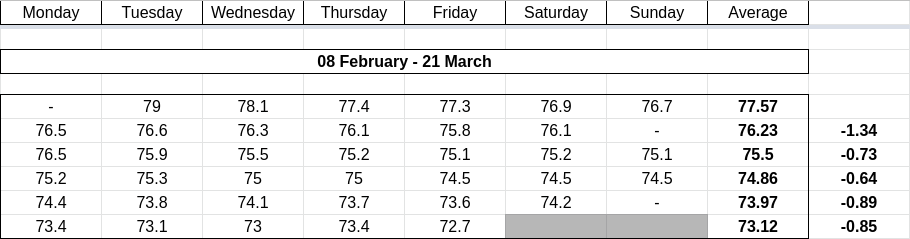
\includegraphics[scale=0.44]{weight-log.png}
		\caption{My weight variation during a cut phase of 6 weeks. All weights are in kg. This phase happened after a cheat weekend, so the initial drop in weight comes from water weight and
                  extra undigested food in the stomach. You can see the average weekly weight going down at a rate of 0.7 - 0.8kg.}
		\label{fig2}
	\end{figure}
	
	Now that you know about bulking \& cutting phase, how long do you do each and how do you plan them? For example, you could be bulking for 4 months and cutting for 1 month.
	However, there is no standard here, it depends on a lot of factors --- what type of bulk you did, how easy you gain fat, what type of cut you are going to do. A common
	approach is to pick your ideal body fat \% (from experience or if you can't, just estimate it looking at pictures) and try to stay close to that value when you bulk \& cut.
	For example my ideal body fat \% is 12\%. I want to end a bulk at +5\% of that value, so 17\%, and a cut at -5\% so 7\% body fat. Since single digit body fat is not that 
	amazing I'm happy to end it around 10\% body fat. If you never lifted before I would recommend starting with a bulk (to gain muscles, increase your metabolism and train your
	body to burn fat easier) for 3-4 months. After this bulking phase, I would cut for however long it takes me to get down to 10\% (could be 1 month or even 5+). After my cutting
	phase is over I would switch again to bulking until I hit 17-20\% then cut down again to 10\% and so on. Another thing to keep in mind is that you might want to end a cutting
	phase in a certain time of the year, for example before summer and then maybe maintain it over summer. This is also possible, you're in charge of however you want to split your
	bulking, cutting and maintenance phases. I would normally bulk over winter, like most people do and start my cutting phase in time to get down to 10\% for the summer. I usually
	start my cut beginning of March to reach my goal by June. A more detailed explanation: let's say I am at 80kg at an estimated 17\% body fat --- this means 66.4kg lean mass and
	13.6kg of fat. To get down to 10\% keeping my lean mass means I have to go down to 73.8kg (66.4kg lean mass and 7.4kg of fat), this means I need to lose 6.2kg of fat. I know I 
	feel comfortable with a diet where I lose 0.7kg per week. Doing the math, this means I need to diet for 8.9 weeks. Knowing that it gets harder to lose fat as you drop body fat
	\% and that my cheat days will set me back quite a bit, I think 12 weeks is a safe bet for me to reach my goal physique, this means I have to start my cutting phase
	start of March to get in shape by June! Even if I don't hit my goal of 10\%, I will be in pretty damn good shape for the summer.

	\section{Metabolism and Adaptive Thermogenesis}
	
	When people say metabolism they usually mean BMR, which is the amount of energy you normally need in a day without extra physical activity. I talked about BMR before, and 
	that it should depend on mass and body fat percentage. When people say they have a fast or slow metabolism I take it with a pinch of salt, because I know it should mostly depend
        on mass and body fat percentage. What I know however from experience is that I'm really bad at estimating how many calories I eat in a day. If everyone would track exactly how
        many calories they eat and how much they burn through exercise then the BMR values should be in accordance with the formulas described above. While this is true for most people,
        BMR can actually change for the same individual at the same mass and body fat percentage. Remember when I said that the energy your body needs to produce heat makes up most of
        BMR's value? It turns out your body can change how much heat it produces (this has nothing to do with your body's temperature, you just radiate more or less heat in the surrounding
        environment) which can affect BMR. This happens usually if you are at a caloric deficit or surplus for a longer period of time, your body will try to adapt to your new intake. This
        process is called adaptive thermogenesis
        \footnote{\href{https://www.ncbi.nlm.nih.gov/pmc/articles/PMC3673773/}{Adaptive thermogenesis in humans article}}, or metabolic damage
        \footnote{\href{https://www.youtube.com/watch?v=bLboowVr2DM}{VitruvianPhysique on metabolic damage on Youtube}}
        \footnote{\href{https://www.youtube.com/watch?v=VVF64oQ3yZk}{Greg Doucette on metabolic damage on Youtube}}.

        If BMR adjusts to your diet then how can you ever lose weight? This is not as bad as it sounds and it won't keep you from losing weight. From my experience, this metabolic damage is
        not enough to keep you from losing weight. The BMR changes are really slow and there is always a limit to how low it can get. Notice that as you lose weight you'll also burn less
        calories for movement since you have less mass, so to keep a steady weight loss pace you need to continuously adapt either your diet or your cardio. Eating less also means less
        calories burned, since it takes a bit of energy for your body to process the food you eat. This is called the thermic effect of food
        \footnote{\href{https://en.wikipedia.org/wiki/Specific\_dynamic\_action}{Thermic effect of food on wikipedia}}. You can see the energy required to break down carbs, proteins and
        fats in Table \ref{table1}. This is usually one of the reason people recommend food high in protein for diets, since they have less calories than advertised. The fact that it takes a lot of
        energy to break them down should also make you feel satiated for longer period of time. I will discuss high protein diets later in the book. 
        Going back to metabolic damage, the good news is that it's not permanent
        and it has been proven to recover after you increase your caloric intake again.

        \begin{table}
          \centering
          \begin{tabular}{|l|c|}
            \hline
            \textbf{Macronutrients} & \textbf{Energy it takes to break it down}  \\
            \hline
            Proteins & 20-35\% of calories ingested \\
            \hline
            Carbohydrates & 5-15\% of calories ingested \\
            \hline
            Fats & 5-15\% of calories ingested \\
            \hline
          \end{tabular}
          \caption{Thermic effect of food}
          \label{table1}
        \end{table}

        I've never had any issues with my weight getting stuck at a certain value. I would advice against going too low in caloric intake, whenever I did that I would feel like crap with no energy.
        A better approach is to just increase the cardio you are doing in a day, just run more to burn more calories. Even if you do more cardio, stay at a comfortable deficit overall, being in
        a big deficit will result in you losing muscles, which will decrease BMR by quite a bit. As a final note, I don't think you can get stuck while doing cardio and training to build muscle
        (e.g. by lifting weights), if you eat too much you'll end up gaining more muscle which will increase your caloric maintenance value (also called set point) which should result in
        being at a deficit eventually if you keep eating the same.


        \section{Intermittent Fasting}

        You might have heard of Intermittent Fasting
        \footnote{\href{https://www.healthline.com/nutrition/intermittent-fasting-guide}{Intermittent fasting on Healthline}}
        before. This is a diet where you allow yourself to eat only in a specific time interval (for example from 1pm until 9pm --- this means skipping breakfast).
        I've heard many people saying how good this diet is for losing weight. A diet like this could work because it's harder to overeat in the 8h you are allowed to.
        I tried it in the past too and found it good for me. In my case it worked because I find it easier to stay hungry in the morning --- I usually drink 1-2 cups of coffee
        in the morning and this suppresses hunger. I also feel I can focus better when I don't eat in the morning so I felt great overall. Some would argue that it's also good
        to train in the morning on empty stomach, since your body is forced to go to fat stores to get the energy it needs (I would assume this to be the case if your glycogen
        stores are depleted, so maybe while doing a keto diet). Personally I don't think it really matters when you exercise, as long as you are at an overall deficit, and it
        might be easier to exercise after you had something to eat. The thing that I realised however is that if you train to build muscle, intermittent fasting might
        not be the best option for you. When you lift weights you damage the muscle, so a repair process will start to take place, also known as muscle protein synthesis.
        This process is known to take up to 36h
        \footnote{\href{https://pubmed.ncbi.nlm.nih.gov/8563679/}{The time course for elevated muscle protein synthesis following heavy resistance exercise}}, or even 48h
        \footnote{\href{https://pubmed.ncbi.nlm.nih.gov/11255140/}{Exercise, protein metabolism, and muscle growth}}. While your muscles are being repaired, you
        need to have proteins available in your stomach to go on the muscle. This is why it's recommended to eat something high in protein before going to bed (preferably casein
        protein, which is slow digesting) and also in the morning (whey protein, which is fast digesting). If you skip breakfast and you stay on empty stomach for too long
        then the muscle protein synthesis process will not be optimal. After I realized this I stopped doing intermittent fasting even when cutting down. Some bodybuilders
        also speak against it if you're trying to build muscle
        \footnote{\href{https://www.youtube.com/watch?v=cMZ8Ijq-6Do}{Greg Doucette on fasting on Youtube}}.

        \section{Tracking Calories, Meal Prep, Cooking}

        So now you know your TDEE, you know whether you want to bulk or cut, so you have a caloric intake goal. To hit this goal you have to start counting how much you eat
        every day (as I've said before, I would advice against estimating this, since big errors will make it impossible for you to hit your goal). You can track in multiple
        ways, for example you can read the label of everything you eat and just write it down somewhere. You can also use a phone app to help you with that (for example myfitnesspal
        \footnote{\href{https://www.myfitnesspal.com/}{MyFitnessPal website}} has such a feature). For me this seemed like a big burden, to always remember to log
        every meal and make sure I hit my calories for the day. An alternative would be to make a meal plan: you plan your meals for the week, you cook in advance and then you
        don't need to track anymore. This option worked really well for me, and I felt like it saved me a lot of time and money. However, not everyone enjoys doing this, making a meal
        plan is not straightforward, takes time to perfect and unless you try really hard to diversify it, it could feel a bit boring to eat the same dishes every day. You can
        try having a hybrid between a meal plan and tracking new meals. Just add a few important dishes to your every day plan (most likely something high in protein) and
        have an amount of calories and protein you still need to hit by eating something different every day. I personally don't care that much about eating something completely
        new every single day and I think others have similar feelings, they would have the same meals every other day.

        I will describe how I made my meal plan for myself, but keep in mind this: making a meal plan is not something you do once and that's it. You might make an initial plan
        but this will have to change and adapt until it actually works for you and you're extremely happy and can stick with it. I started by making a spreadsheet with all the
        food I normally like to eat, splitting them into different sections (high in carbs, fat, protein etc) and adding their nutritional values. I then made a table where
        I can adjust the amount of each type of food and it will automatically add the calories and macros for the day. Once I hit how many calories and proteins I need in a day, 
        I'm done. I then proceed to test my meal plan in the following week: do I lose or gain the correct amount of weight? Am I happy with my meal plan? Do I enjoy the meals?
        Does it keep me full and not hungry all the time? If the answer is yes to all these questions, then I'm lucky and I just made the perfect meal plan. If not, then I 
        keep adjusting it, swapping food until I can answer yes to all the questions.
        I made a copy of my meal plan calculator spreadsheet available for everyone online at
        \footnote{\href{https://docs.google.com/spreadsheets/d/1DPH4OQuc6yQf3TdUI1D3m1t4UGaiRP1ptWh5f9Y9Y2U/edit}{Meal Plan Calculator on Google Spreadsheets}}.
        You can copy that spreadsheet to a private one for yourself to edit. Just update the $Food$ column with the food you like, add the macros, add your goals on the
        bottom right then keep adjusting the units in the calculator until you hit your goals! You can see a picture of the meal plan calculator below (Figure \ref{fig2}) and 
        also an example of a day meal plan I made using it for cutting down (Figure \ref{fig4}).

	\begin{figure}[h]
		\centering
		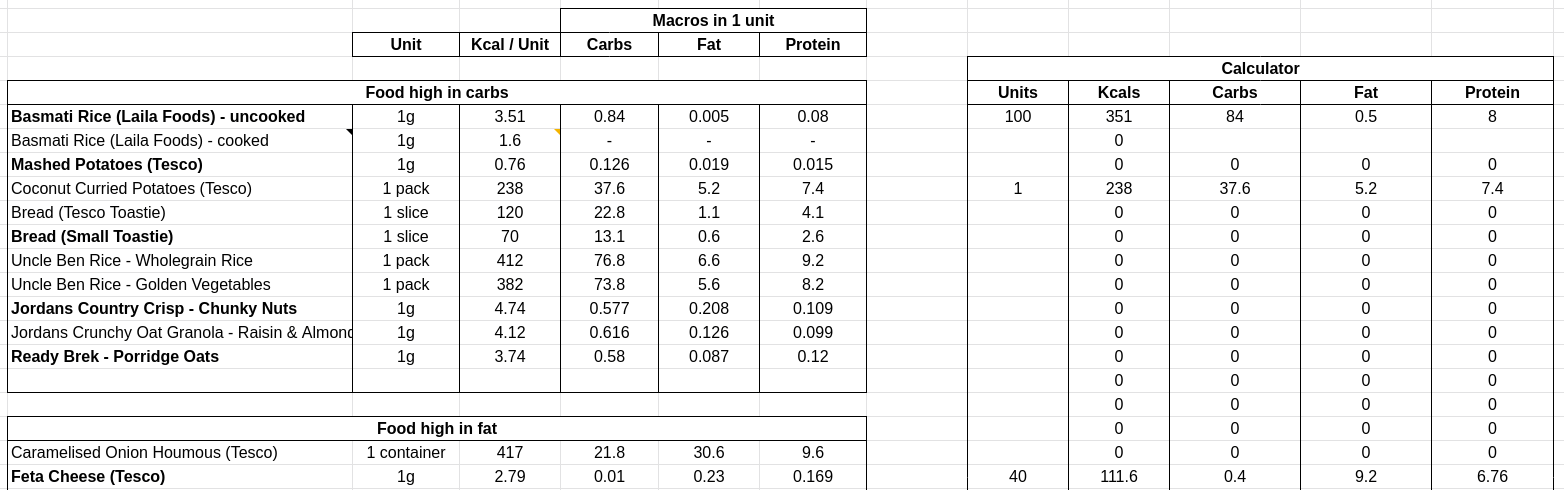
\includegraphics[scale=0.3]{meal-plan-calculator.png}
		\caption{The meal plan calculator I use to create new meal plans. The foods I eat are on the left, I just add the units on the right and it automatically adds everything at the bottom so I can compare it with my goal}
		\label{fig3}
	\end{figure}
        
	\begin{figure}[h]
		\centering
		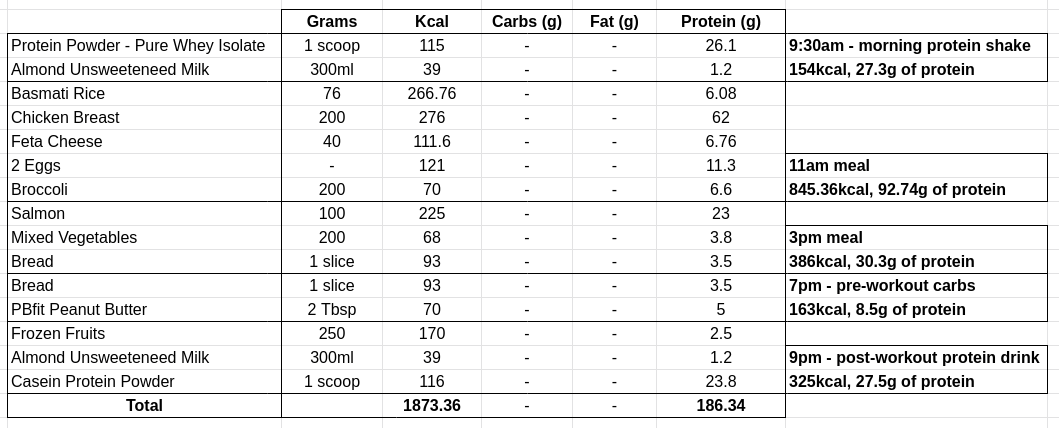
\includegraphics[scale=0.44]{cutting-meal-plan.png}
		\caption{An example of a meal plan I made for cutting down. I used to track carbs \& fat but not anymore}
		\label{fig4}
	\end{figure}

        It might be difficult to decide what amount to use for each type of food. I started from experience (e.g. a typical chicken breast meal I buy
        from the supermarket has around 125g of chicken breast and 125g of rice or something similar). I also had to take into account the preparation process for these
        meals and in what quantities I can buy the groceries. For example, I can find 1kg of chicken breast, so using 200g a day for 5 days is really easy to do --- cook the 1kg
        and split into 5. If I ended up in my spreadsheet with a random odd number for the amount of chicken breast in a day (like 167g), then buying for the week would be
        impossible without throwing some away. So there is a bit of tweaking the numbers until you get everything right. If you want to have different meals on different days 
        you repeat the process until
        you have something planned to eat for each day. In my case I don't mind eating the same thing Monday to Friday, so I cook 5 times the amount of food I would eat in a 
        day every
        Sunday for the next week. On the weekends I allow myself to eat different things, but I try to stick to food high in protein and fiber so I don't end up overeating.
        After I have a meal plan, I move it to a different spreadsheet and label it accordingly.

        Cooking the food is not as hard as you might think. If you're not pretentious with your food then it doesn't require any cooking skills at all. I will describe the way
        I do it, which I think is really fast and for me it tastes good too. In my cutting meal plan I have a few dishes that require cooking: the classic chicken,
        rice and broccoli dish, salmon with bread, vegetables and eggs. I usually buy frozen broccoli/vegetables so I just need to heat them up in the microwave before eating.
        This means I still have to cook the rice, chicken breast, salmon and eggs. For both the chicken breast and salmon I use a slow cooker. Slow cookers
        \footnote{\href{https://crockpot.co.uk/}{Crock-Pot slow cookers}} are great devices
        if you don't have time to cook. They are also really cheap (\textsterling 20-\textsterling 30). I find them an alternative to microwave: instead of buying already 
        cooked meals you can buy frozen
        food instead, throw it in the slow cooker in a similar way you do with the microwave, and later just take it out and it's ready to eat. It does take a rather long time 
        to cook, 4h
        compared to 5min for microwave, so you need to plan in advance. Also usually frozen food doesn't come seasoned so you might want to add spices before you throw it in 
        the slow cooker. Frozen food is also cheaper than pre-cooked meals, so in the long run you end up saving money. In my opinion slow cooked meals taste better than
        microwaved ones, but still fall behind something you'd cook in a pan.

        Going back to my cooking process, I would normally buy 1kg of chicken breast, wash it, put it in the slow cooker with a bit of water and leave it on high for 4h.
        You could do 6h on low but at the end of the day it depends on how much you cook and what slow cooker you own. I realised that 6h on low is too long for my salmon,
        so I now put it for 5h (usually overnight) only. After the chicken breast is cooked I just
        split it into 5 portions (for Monday to Friday). I use a kitchen scale to split it as equal as possible, but sometimes I don't have time for this so I just eyeball it.
        I do the same with the salmon (500g in my case). I don't add any water to the salmon, it has a lot of grease so it will cook just fine. I don't use seasoning but you
        can use if you really want. I use Frank's Red Hot sauce
        \footnote{\href{https://www.franksredhot.com/}{Frank's Red Hot website}} with my meals instead of seasoning.
        The sauce has almost no calories --- it's like liquid salt with a bit of spice. If you don't like spicy, you can probably find low calories sauces out there for your
        taste. I cook the eggs and rice at the same time using a rice cooker. I know how many cups of rice I need to hit the amount I have in my spreadsheet. I did the
        measurements once and and ended up being around 3 cups for 5 days. I rinse (a fancy word for washing) the rice, add it to the rice cooker and add water (in my case I use
        2 cups of water per cup of rice, so 6 cups of water in total). My rice cooker came with a steam tray, so I place 10 eggs (I eat 2 each day) in this steam tray and turn on
        the rice cooker. I leave the eggs for about 18min for the perfect consistency (I like the yolk a bit runny). The rice cooker stops automatically after the rice is cooked.
        It normally takes around 40min. After this is done I split it again into 5 portions using the kitchen scale. I split the food I cook into tupperware
        \footnote{\href{https://igluumealprep.com/}{You can buy meal prep containers online}} and put it in the
        fridge for the entire week. For some of you, eating a meal 5 days after it was cooked might be too much, but personally I had no issues. Yes, the food tastes much better
        early in the week (the rice is fluffier and the chicken breast more tender) and not so great on a Friday. However, I don't really have time to cook midweek. Even if it
        sounds like a lot of steps, I actively spend only 1-2h each Sunday to cook for the entire week and with enough Frank's Red Hot the food tastes amazing to me. It's more
        practical than proper cooking you could say.

	\begin{figure}[h]
		\centering
		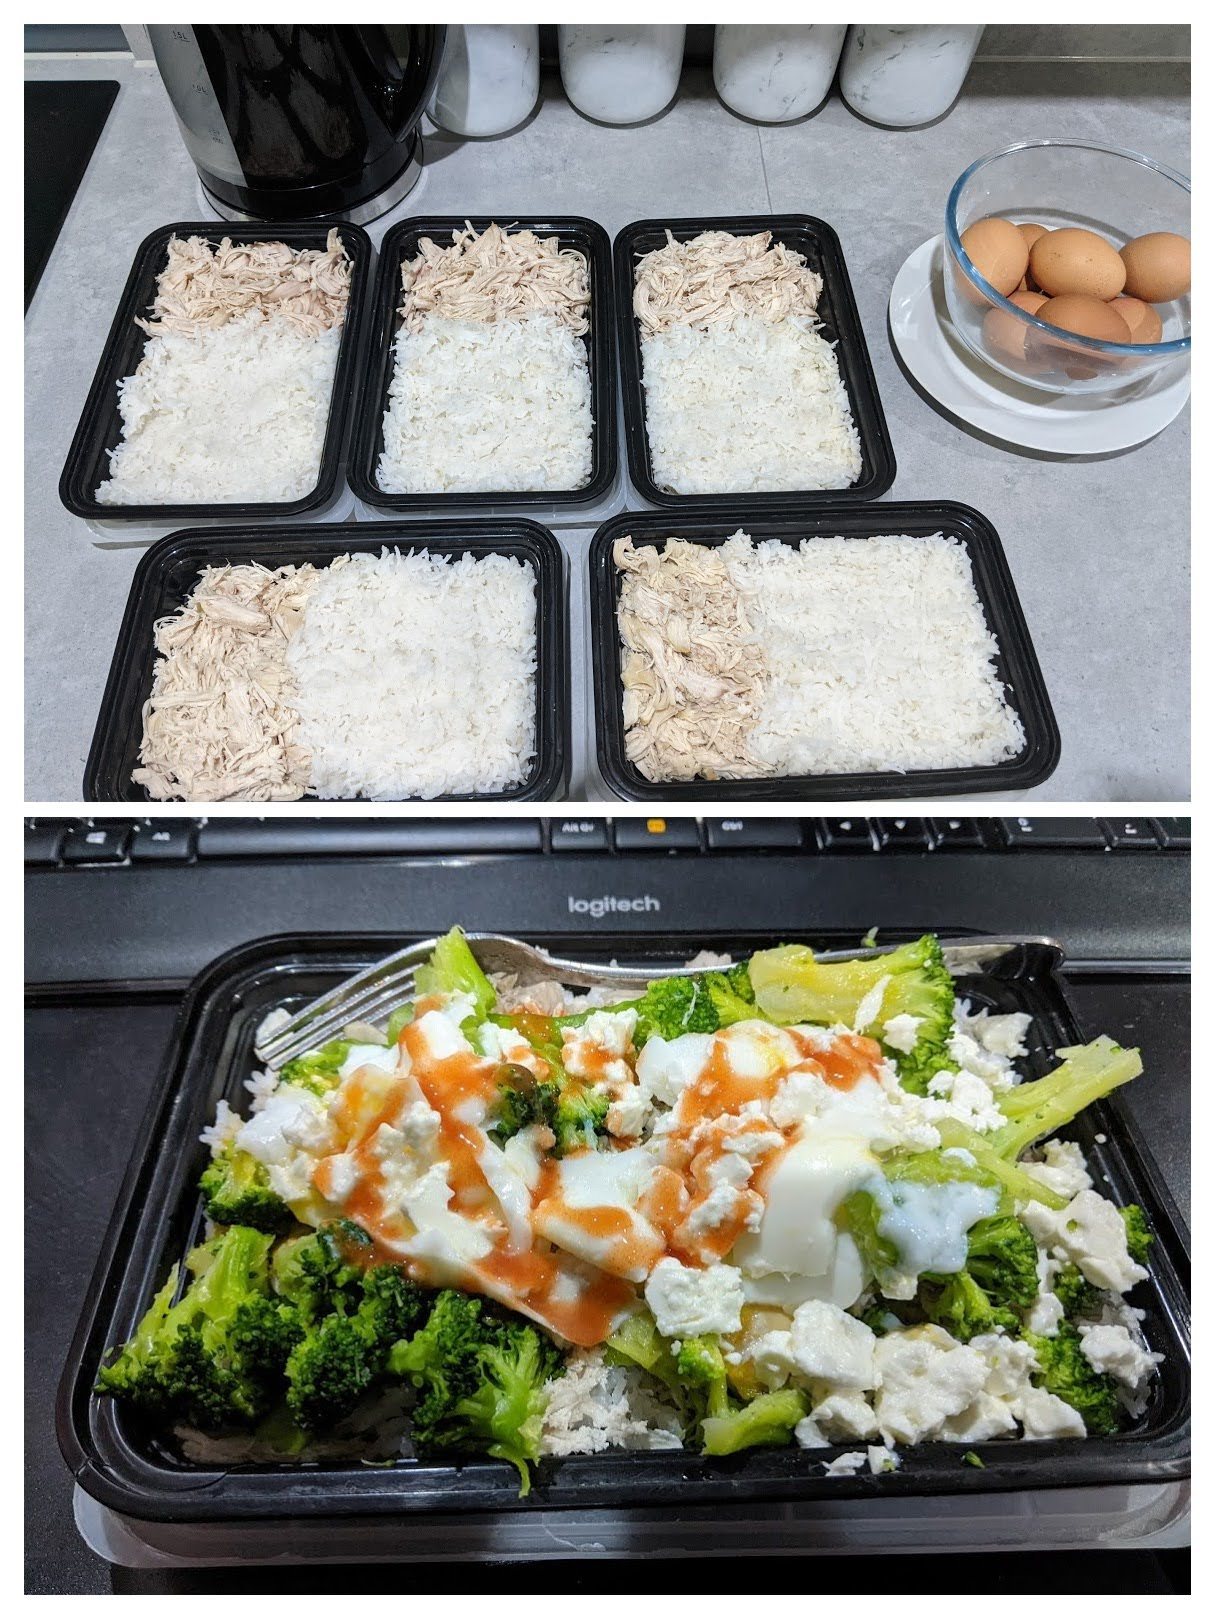
\includegraphics[scale=0.2]{meal-prep.jpg}
		\caption{Cooked rice, chicken breast and eggs for the entire week (top) and one meal of chicken, rice \& broccoli (bottom)}
		\label{fig5}
	\end{figure}

        From what I've seen a lot of people seem to struggle with diets because they get hungry. I personally don't have a big issue with this, but I've seen a lot of people in 
        the fitness industry advocating meals high in protein and fiber. The idea is that both proteins and fiber take a long time to digest, so you will not feel hungry while
        this process is happening, even if you don't eat that many calories. I discussed this previously when I talked about the thermic effect of food.
        I tried cooking meals high in protein and I agree that some of them are super filling. For example egg whites are
        one of the most filling dishes I had and they are low in calories and high in protein. You can find egg whites liquid boxes
        \footnote{\href{https://twochicks.co.uk}{Two Chicks egg whites}} that you can cook straight in
        the pan or make something like protein pancakes
        \footnote{\href{https://www.youtube.com/watch?v=aDJ8K_gqzdI}{Greg Doucette with protein pancakes on Youtube}}. 
        I find a lot of high protein recipes online, mostly on YouTube. Examples of youtubers with such recipes: Greg Doucette
        \footnote{\href{https://www.youtube.com/playlist?list=PLNAZHiu0ASAprWRUxQHAiHG1FhlJbyeIm}{Greg Doucette's anabolic kitchen on Youtube}}
        (he also has a cookbook full of such recipes
        \footnote{\href{https://www.gregdoucette.com/products/cookbook-2}{Greg Doucette's cookbook}}; haven't
        tried it so I can't say if I recommend it or not), The Iron Musket
        \footnote{\href{https://www.youtube.com/channel/UC3Pec4Q-1CEc9WXjVk2z6Bg}{The Iron Musket on YouTube}}
        (a lot of high protein ice creams recipes, as you can see in Figure \ref{fig6}), Sam Does Fitness
        \footnote{\href{https://www.youtube.com/channel/UC8JUC4wItW2EwpeMkCSyRUw/}{Sam Does Fitness on YouTube}}, Remington James
        \footnote{\href{https://www.youtube.com/channel/UCO9Rhj_x_GgJl-Ria7257EA}{Remington James on YouTube}}, Will Tennyson
        \footnote{\href{https://www.youtube.com/channel/UCB2wtYpfbCpYDc5TeTwuqFA}{Will Tennyson on YouTube}} and many more.

	\begin{figure}[h]
		\centering
		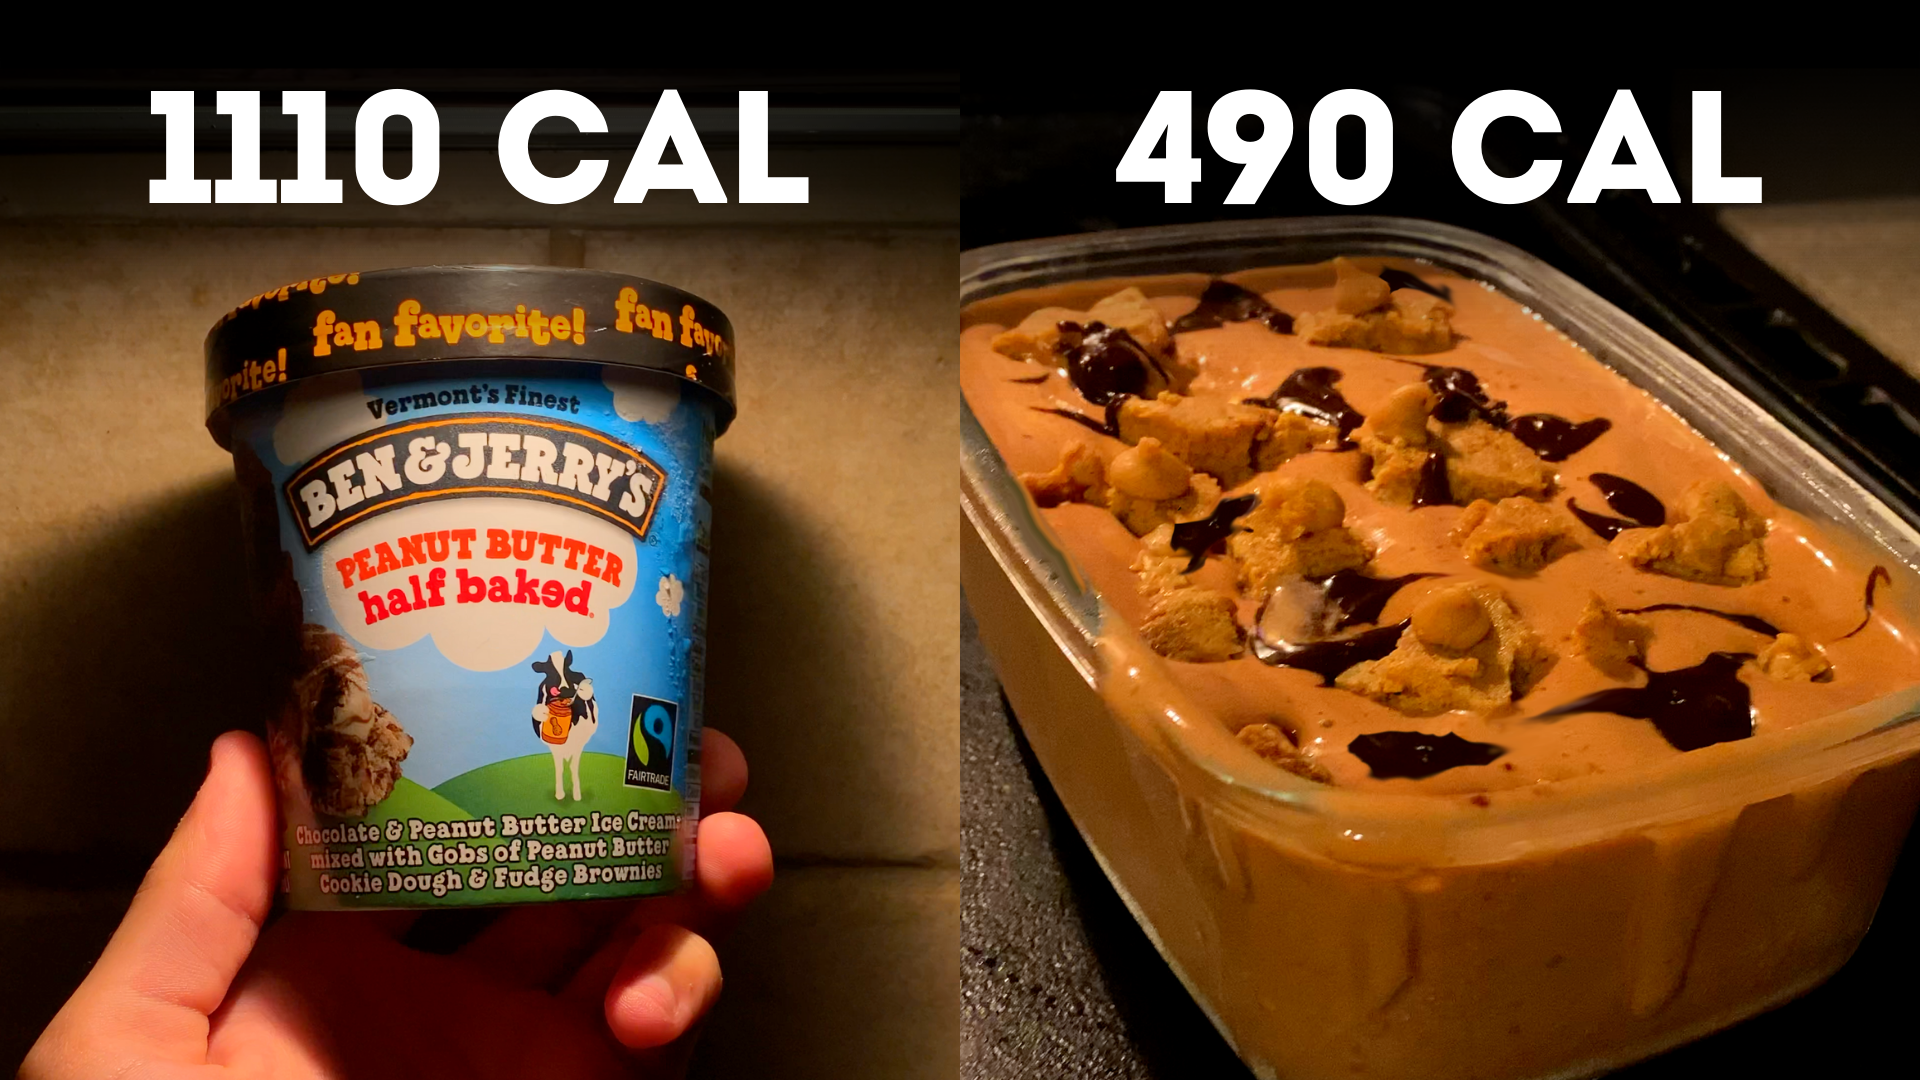
\includegraphics[scale=0.24]{protein-ice-cream.png}
		\caption{Example of a protein ice cream recipe from The Iron Musket YouTube channel. Notice it's much bigger than an actual ice cream tub and half the calories}
		\label{fig6}
	\end{figure}

        Another struggle with diets are cravings. Not eating pizza in a long time would make me want a pizza slice so bad. The good news is that there are high protein
        alternatives to a lot of popular dishes you can cook, and they seem to kill cravings for me while on a diet, which is perfect! I can have protein pizza, protein
        ice cream, even low fat peanut butter
        \footnote{\href{https://pbfit.com/}{PBfit, low fat alternative to peanut butter}} all while cutting. I can make a small pizza for less than 300 calories using Lo-Dough base
        \footnote{\href{https://lodough.co/}{Lo-Dough website}} and EatLean cheese
        \footnote{\href{https://eatlean.com/}{EatLean website}} that still tastes really
        good and looks amazing (Figure \ref{fig7}).
        
	\begin{figure}[h]
		\centering
		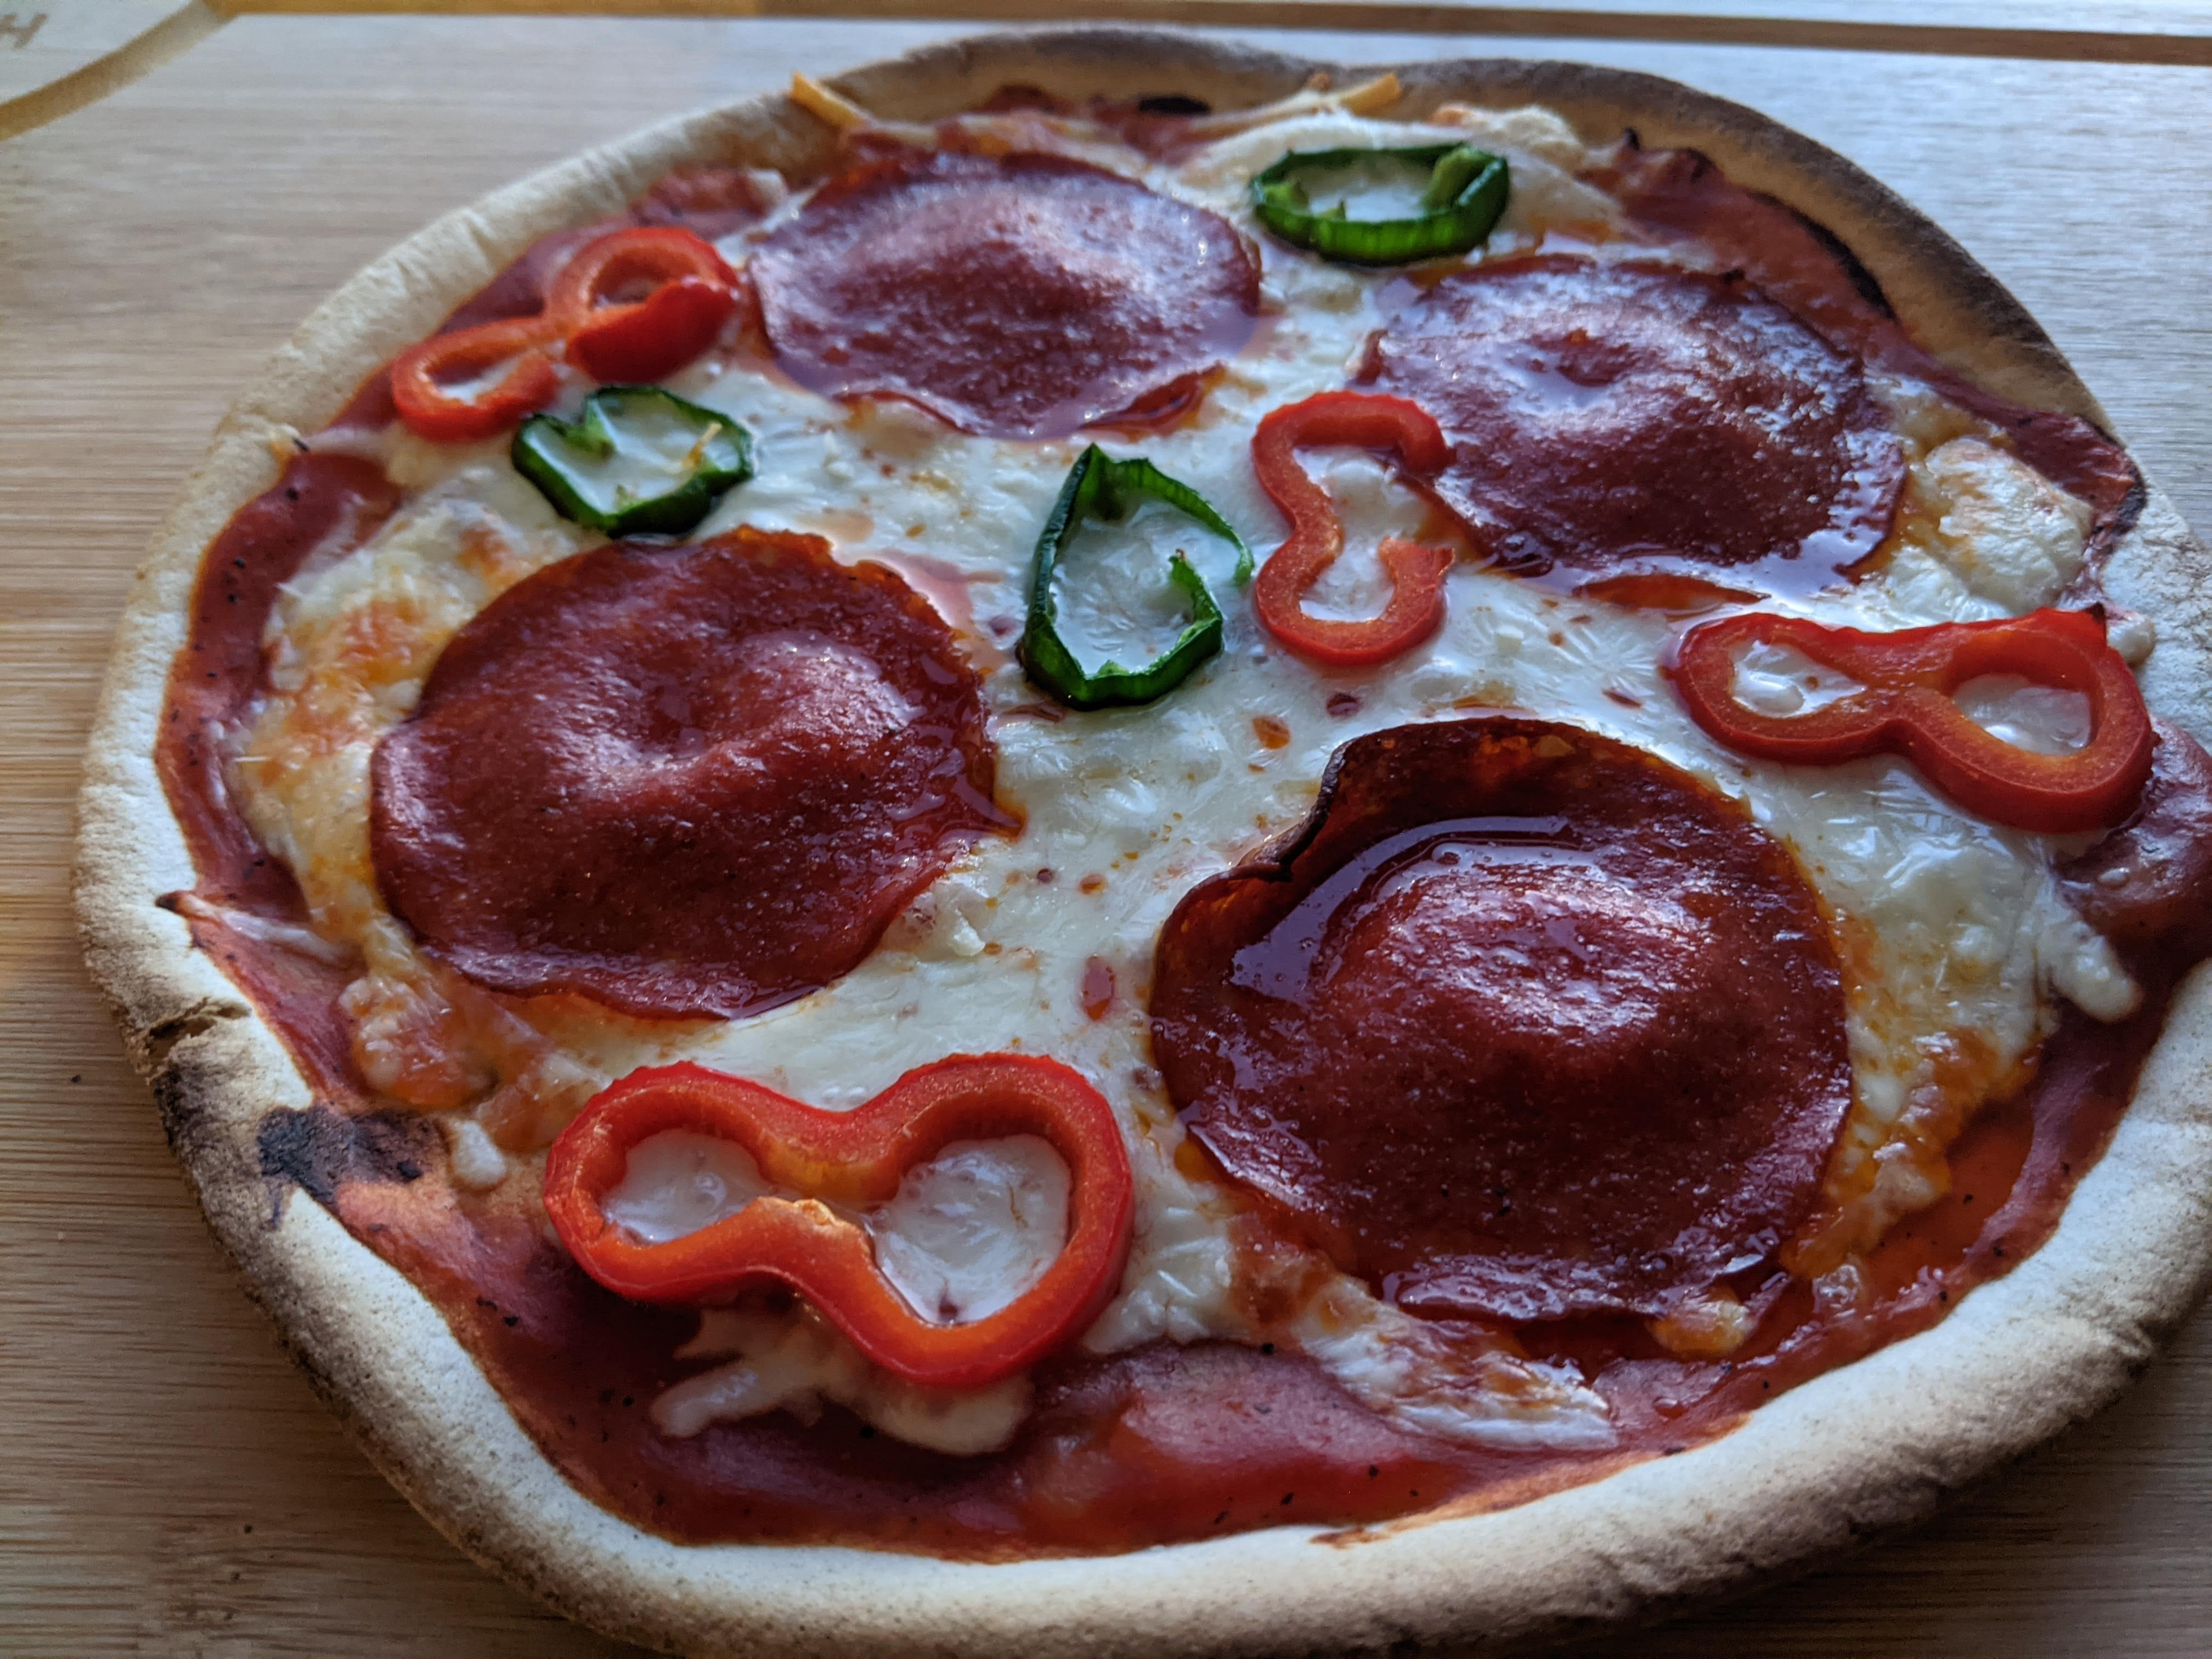
\includegraphics[scale=0.113]{protein-pizza.jpg}
		\caption{Protein pizza for less than 300 calories. It's small but it does the job when it comes to stopping cravings}
		\label{fig7}
	\end{figure}

        \section{Supplements}

        A good diet and workout plan should give you really good results. On top of this, some people advice that taking different pills or powders can help you get even better results.
        I take some of these supplements myself, however I never tested what actually works and what not since I'm getting results anyway and it's hard to tell what really makes a difference.
        I will just try to give a brief overview.

        Protein powders --- these are powders made of different types of proteins. Most of the time you can get the same proteins from food, but if you struggle to hit your protein goals for
        the day or if you want a quick meal alternative then they might be for you! You can find different types of protein powders, such as whey protein (faster to break down) and casein
        (slower to break down). You mix these powders normally with water or milk (I prefer unsweetened almond milk for the consistency and low amount of calories) and drink them.
        I use whey protein powder in the morning (1 scoop or 26g of proteins) since I want a quick intake of proteins before I get to eat anything else. You can get whey protein naturally
        from milk which has both whey and casein in different proportions based on what type of milk it is. I also use casein protein powder (1 scoop)
        in the evening so that I have some protein in my stomach when I go to bed. I also add creatine to this casein protein shake, which I will discuss later. You can also get casein naturally
        from cheese, which is made from milk after removing the whey protein.

        Branched-chain amino acids (BCAAs)
        \footnote{\href{https://www.healthline.com/nutrition/bcaa}{BCAAs on Healthline}} --- proteins are made of amino acids. There's 20 different types of amino
        acids out there. From these 20, we need only need 9 in our diet to be healthy
        \footnote{\href{https://en.wikipedia.org/wiki/Protein\%E2\%80\%93energy\_malnutrition}{Protein-energy malnutrition on wikipedia}}. We normally get all of them from food
        high in protein such as milk, eggs, meat and so on. From these 9 amino acids, 3 of them are called branched-chain amino acids: leucine, isoleucine and valine. People say these 3 amino acids
        are better at building muscles than the other ones. Most protein powders already have them, for example both whey and casein proteins contain all 3 (they actually contain all 9, which is
        why they are called complete proteins). BCAA powder only has the 3 amino acids I mentioned. Personally I've never tried powders with BCAAs only and I don't know if it's better than having
        complete proteins such as whey or casein. I've also seen people claiming that BCAAs don't have calories, which is hard to believe since they are amino acids just like the other ones which
        make up proteins, and proteins do have calories!

        Glutamine
        \footnote{\href{https://www.healthline.com/nutrition/glutamine}{Glutamine on Healthline}} --- this is another amino acid, making up proteins just like BCAAs. However Glutamine is
        not part of the 9 essential amino acids, it is only needed under certain circumstances (for example injury or illness). Glutamine is found in whey \& casein proteins too. You can also get
        it from certain types of food (eggs, milk). Glutamine has been shown to help with recovery. Again I never took glutamine by itself, just from foods and my whey and casein protein shakes.

        Creatine
        \footnote{\href{https://www.healthline.com/nutrition/what-is-creatine}{Creatine on Healthline}} --- this is a supplement everyone believes to work. There have been studies
        showing it works, every bodybuilder
        \footnote{\href{https://www.youtube.com/watch?v=W9Kas49cNnU}{Greg Doucette on supplements on YouTube}}
        \footnote{\href{https://www.youtube.com/watch?v=6Xj1MNJK-iA}{VitruvianPhysique on supplements on YouTube}}
        I watch also approves of it. I take it as well, however I can't say how much it helped me. When I started taking it I was doing a bulk, relatively
        early in my lifting career so I was increasing the weight I can lift in the gym quite frequently anyway. Creatine is stored inside your muscle, and it's used with glycogen and fat to produce
        adenosine triphosphate (ATP) which makes your muscle contract. You normally get it from various types of meat (tuna, steak) but you can also take it as a supplement. Some people say that
        the amount you can get from food is not enough and supplements are needed for an optimal amount of creatine stores in your muscles
        \footnote{\href{https://www.youtube.com/watch?v=sREg8GrkPio}{Athlean-X on supplements on YouTube}}.
        Taking it as a supplement should help with ATP production, which should give you more strength and endurance in the gym.
        You can buy creatine in powder form and mix it in your drink. I normally take it after gym in the evening when I mix it with casein protein powder and unsweetened almond milk as my
        post-workout drink. There's various theories on when it's best to take it (usually post workout)
        \footnote{\href{https://www.healthline.com/nutrition/best-time-for-creatine}{When to take creatine on Healthline}}.
        The recommended intake is 3-5g per day, which should be 1 scoop with the scoop provided in the package. It normally takes time for the creatine stores in your muscle
        to increase from the supplement you take (around 2 weeks). This is why some bodybuilders do something called creatine loading
        \footnote{\href{https://www.healthline.com/nutrition/creatine-loading-phase}{Creatine loading on Healthline}} --- taking 20g of creatine every day for 5-7 days to speed up the process,
        then going back to 3-5g a day.

        One thing worth mentioning about creatine is that it has been linked to hair loss
        \footnote{\href{https://pubmed.ncbi.nlm.nih.gov/19741313/}{Article on creatine effects on DHT}}
        \footnote{\href{https://www.youtube.com/watch?v=NgcfEMu_WSE}{VitruvianPhysique on creatine and hair loss on Youtube}}.
        Most guys will experience male pattern baldness
        \footnote{\href{https://www.healthline.com/health/male-pattern-baldness}{Male pattern baldness on Healthline}} as they grow old. This happens because of testosterone (more specifically
        dihydrotestosterone or DHT) which gets attached to the hair follicle causing it to die out slowly. This normally happens with the hair on the top and not sides or back, since it's believed that
        the hair there is immune to DHT. In hair transplant operations, hair follicles from the back of the head are extracted and placed on the top, where they start growing again.
        There are also options to try and prevent the male pattern baldness from happening, which only works if you start using them before the hair follicle dies. If it died then 
        the only solution is hair transplant. Some of these options include applying minoxidil solution
        \footnote{\href{https://en.wikipedia.org/wiki/Minoxidil}{Minoxidil on Wikipedia}} on the top of your head, taking a pill called Finasteride
        \footnote{\href{https://en.wikipedia.org/wiki/Finasteride}{Finasteride on Wikipedia}} and others
        \footnote{\href{https://www.healthline.com/health/dht}{DHT article on Healthline}}. Before you take anything you should book a consultation with a doctor or hair loss specialist
        (there's other causes to hair loss than DHT, some of these meds have side effects etc).
        Back to the topic of creatine and hair loss, usually training in the gym will boost your testosterone. Any boost in testosterone can accelerate male pattern baldness. While creatine is linked
        to increase in testosterone, I assume that anything that helps you lift more weights should indirectly help increase testosterone so it's not really a surprise.
        Personally I haven't noticed hair loss after I started using it, but I do use minoxidil every day.

        Multivitamins --- a lot of people recommend taking multivitamins. Working out weakens your immune system right after exercise
        (T-cell production drops for up to 6h, after which it should return to normal)
        \footnote{\href{https://pubmed.ncbi.nlm.nih.gov/17037088/}{Article on immune system response to exercise}}.
        This time interval in which your immune system is weakened is also called the \textit{open window}
        \footnote{\href{https://pubmed.ncbi.nlm.nih.gov/20839496/}{Article on open window after intense exercise}} and you are more likely to get sick during this time.
        Multivitamins pills are known to help the immune system, which is one of the reasons they are recommended. If you manage to take your daily intake of vitamins and minerals from food I think
        you should be fine.
        However, I find it harder to track what vitamins and minerals I eat in a day, so I'm taking multivitamins pills daily.

        Omega 3 --- this usually comes from fish oil. It is believed that fish oil should help with recovery (e.g. joint recovery, inflammations). It's also recommended for a lot of different reasons
        \footnote{\href{https://www.healthline.com/nutrition/fish-oil-bodybuilding}{Fish oil on Healthline}}. I personally eat fish almost every day, and when I don't, I take
        omega 3 supplements in form of pills.

        Glucosamine Chondroitin
        \footnote{\href{https://www.healthline.com/nutrition/glucosamine}{Glucosamine on Healthline}} --- this supplement is supposed to help with inflammations from exercise.
        I had a tendon inflammation in my right arm and tried this supplement in the form of pills and it did nothing to help me recover. There is information out there that it should help with
        the healing of tendons, however that was not the case for me. The only thing that helped me recover was a long absence from working out.

        Pre-workout drinks --- you must've seen pre-workout powders in shops. They are supposed to help you get energized before a workout. As such, they usually contain high amounts of caffeine
        (the equivalent of 2-3 cups of coffee for the weaker ones, and even more for the stronger ones). They also have other stuff in them, such as creatine, carbs, beta-alanine
        \footnote{\href{https://www.healthline.com/nutrition/beta-alanine-101}{Beta-alanine on Healthline}}, citrulline
        \footnote{\href{https://www.healthline.com/nutrition/citrulline-supplements}{Citrulline on Healthline}} and so forth. I personally don't take pre-workout, running on the treadmill
        before doing my workout wakes me up and puts me in the mood to exercise. I also consume a large amount of coffee each day, so adding the caffeine from pre-workout will be bad for my health.
        If you struggle to get motivation to workout then maybe pre-workouts are for you. You can read more about pre-workout supplements at healthline
        \footnote{\href{https://www.healthline.com/nutrition/best-pre-workout-supplements}{Pre-workout supplements at Healthline}}.

        Intra-workout drinks --- not as famous as pre-workout, but some people use them too. Intra-workout means you have to drink it while you exercise. I get the idea of drinking something every 30min
        if your workout is too long. As previously discussed, if you perform high intense activity such as lifting weights, your body will use glycogen for energy, which will deplete the glycogen stores
        over time. There was a study where individuals were given drinks with low amount of carbs every 30min while they were working out, showing results that it actually helped them to a better
        workout. I believe intra-workout powders work in a similar way, they contain small amounts of carbs that should help you keep going. Consuming carbs every 30min or so is also
        called \textit{carbing up}. I've seen many bodybuilders carbing up while doing a workout (e.g. eating a rice cake every now and then).

        I just want to reiterate again with what supplements I use: whey protein powder in the morning, casein protein powder in the evening, creatine, multivitamins and if I don't eat any fish
        in a day I also take omega 3 capsules. Because I sweat a lot I end up
        losing a lot of sodium when exercising. I noticed that drinking water with a bit of salt (or stock cubes) makes me feel better
        than drinking plain water, although I don't consider this a supplement. There is also a website that claims to help with info on supplements --- examine.com
        \footnote{\href{https://examine.com/}{Examine website}}.
        I'm listing all the supplements discussed in this section as a list, for easier referencing:

	\begin{enumerate}
		\item Protein powders (whey \& casein)
		\item Creatine
		\item Omega 3
		\item Multivitamins
		\item BCAAs
		\item Glutamine
		\item Pre-workout (caffeine, creatine, beta-alanine, citrulline, carbs etc)
		\item Intra-workout (carbs)
		\item Glucosamine Chondroitin
	\end{enumerate}

        \section{Performance Enhancing Drugs}

        I've already discussed performance enhancing drugs (PEDs) in the previous section, since the definition is a bit broad: anything that gives you a mental or physical edge while exercising or
        competing. To that extent even caffeine or creatine are PEDs. However, when people in the fitness industry talk about PEDs they usually refer to either anabolic steroids or selective androgen
        receptor modulators (SARMs) which I will discuss in the next sections. Personally I've never tried any of these but I will describe what I've heard and read about them.
        Both steroids and SARMs have been used with great results: expect to gain muscles at least 5 times faster than training natural, all while cutting down fat
        \footnote{\href{https://www.reddit.com/r/nattyorjuice/comments/c0mak1/physique_before_usage_of_the_steroids_is/}{Example of anabolic steroid transformation in 20 weeks}}.
        They are commonly used in bodybuilding competitions to make the competitors bigger and leaner at the same time. However, they can have serious side-effects, including death. In fact quite a lot
        of bodybuilders have died because of too much steroid use
        \footnote{\href{https://fitnessvolt.com/bodybuilder-deaths-heart-attack/}{21 Bodybuilders who died of heart attacks}}.
        The reasons people usually decide to use PEDs are

	\begin{enumerate}
		\item Being able to get really low in body fat \% (for example close to 5\%). This is usually useful for bodybuilders that compete in shows, where being leaner gets you a higher place
		\item Being able to keep growing in size even after training for a long time / reaching your genetic potential
		\item Being able to gain muscles and cut fat at the same time, or get lean really fast
		\item Being able to eat junk food and drink alcohol while staying in shape
	\end{enumerate}

        However the side-effects can be

	\begin{enumerate}
		\item Impotence and testicular shrinkage (for men)
		\item Brain \& liver cancer
		\item Heart \& kidney disease
		\item Development of breast tissue for men (Gynecomastia)
		\item Deep voice or hair growth (facial or body) for women
		\item Yellowing of eyes and skin
		\item Depression
		\item Severe acne
		\item Bad breathe
		\item Violent behaviour
		\item Death
	\end{enumerate}

        Since both steroids and SARMs increase testosterone in the body, your body will start producing less testosterone naturally. As a result for guys, the testicles will start to shrink, which could
        lead to impotence. This is also why testosterone is used as a male contraceptive since it reduces sperm count
        \footnote{\href{https://www.webmd.com/sex/birth-control/news/20090506/testosterone-tested-as-male-contraceptive}{Testosterone as a male contraceptive on WebMD}}.
        What people usually do to avoid this and other permanent damages is to have cycles of steroid use for around 8 weeks, followed by a post cycle therapy (PCT)
        \footnote{\href{https://musclerage.co.uk/supplements-blog/pct-a-comprehensive-guide-to-post-cycle-therapy-2020/}
        {Website on PCT}}
        of 4 weeks. During PCT you make sure your body will go back to producing testosterone in normal levels. This usually means just taking a bunch of medication to help your body get back
        to normal, such as: Tamoxifen (Nolvadex, 20mg a day), testosterone boosters (e.g. Metatest from Metabolic Nutrition or InnovaPharm Stage 1), human chorionic gonadotropin (hCG),
        Clomifene (Clomid, 50mg every day), Letrozole (Femara). Most of these are available on doctor prescription only. Tamoxifen is used for light cycles, that are short in length and with low
        dosage, for example a PCT with Tamoxifen could mean taking 30mg a day for the first week, 20mg a day for the second, 10mg for the last one (first week is 1 week after end of cycle).
        hCG is used for stronger cycles, that take longer than 8 weeks and with higher dosage of substances. This is a solution you have to inject. An example of hCG PCT is doing 1,000 units
        on the first day, take a day off, another 1,000 units, another day off, 750 units, day off, 750, off, 500 and so on until the whole 5,000 vial is finished (you will need
        Tamoxifen as well afterwards).
        Since it takes some time for your testosterone levels to go back to normal, you might feel like crap during PCT --- no strength, depression,
        no sex drive, you lose muscle mass etc. It's considered good if you manage to keep at least half the muscle mass you gained while on cycle.
        
        Another common side effect is an increased level of estrogen in the body. This happens because some testosterone is converted to estrogen in a process called Aromatization
        \footnote{\href{https://www.blaineywellness.com/wp-content/uploads/2016/08/testosterone-and-aromatization-how-to-avoid-excess-estrogrogen-production.pdf}
        {Testosterone and aromatization: how to avoid excess estrogen production}} that keeps hormonal levels in balance. This will cause men to develop breast tissue just like women, and get 
        \textit{puffy} nipples, as seen in Figure \ref{fig8}. To avoid these problems people usually take aromatase inhibitors (AIs) like Aromasin (Exemestane) --- 12.5mg once a day, or
        Arimidex (Anastrozole) --- 0.5mg once a day, or even hCG.

	\begin{figure}[h]
		\centering
		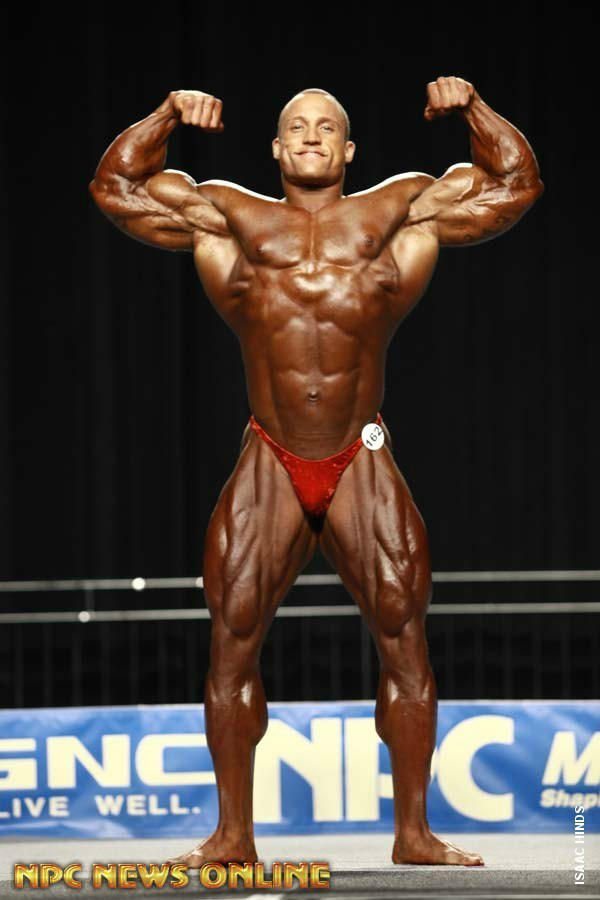
\includegraphics[scale=0.45]{gyno.jpg}
		\caption{Example of gyno on bodybuilder - look at the nipple area. Picture taken from twitter}
		\label{fig8}
	\end{figure}

        One last common side-effect is an enlarged heart (cardiomegaly). This can lead to heart failure and as I previously mentioned there's quite a few bodybuilders who died because of this
        \footnote{\href{https://www.menshealth.com/trending-news/a19541843/bodybuilder-rich-piana-autopsy-report/}{Article on Rich Piana's death}}
        \footnote{\href{https://www.dailytelegraph.com.au/news/nsw/bodybuilder-aziz-zyzz-shavershian-killed-by-heart-defect/news-story/57bbadf89f78c5d678d4df0c5b35d0d5}
        {Zyzz dies from heart attack}}.
        
        Even with all these serious side-effects, a lot of people do end up using steroids or SARMS. In fact, most bodybuilders who compete use them
        \footnote{\href{https://www.youtube.com/watch?v=k8mBn3Dp7h4}{Brandon Harding - good example of what he's using to compete on Youtube}}
        and a lot of fitness ``\textit{influencers}''
        you see on instagram use them as well. Even actors who prepare to play certain muscular characters are using them. If you do decide to use them, it probably makes sense to talk to a
        doctor first and get your blood tested throughout the process. You might also want to take supplements to protect your liver, heart etc
        \footnote{\href{https://www.htltsupps.com/collections/capsules/products/liver-support/}{Liver support supplements from HTLT Supps}}
        \footnote{\href{https://theanabar.com/products/shield?variant=33058384969837/}{Shield from Anabar}}.

        One last point to make about steroids and SARMs is that they are illegal in a lot of countries, so people might buy them from dealers in the gym or from edgy websites. This usually means
        that you might not be getting what you paid for. It also makes them rather expensive. There was a study done where they bought SARMs from various websites selling them and the result was that
        only 30\% of the supplements contained what they actually say they contain.
        \footnote{\href{https://ergo-log.com/20-sarm-supplements-tested.html}{20 SARM 'supplements' tested on ergo-log}}
        Most of them were underdosed, some even had nothing in them, or containing other chemicals.

        \subsection{Testosterone}
        
        Before talking more about anabolic steroids and SARMS, I just want to give a brief overview of testosterone. I mentioned before that testosterone plays an important role in building muscles.
        Testosterone is the male sex hormone, it's produced by testicles for men and ovaries for women (women have testosterone too, just in much lower quantities).
        The amount of testosterone in your body is measured in $ng/dL$, although sometimes you can find $nmol/L$ which can be converted to $ng/dL$ by multiplying the value with $28.85$.
        The average male has between 300 and 1,000 $ng/dL$ while for women it's only between 15 and 70 $ng/dL$. The amount of testosterone your body produces also declines with age, but not by much
        \footnote{\href{https://pubmed.ncbi.nlm.nih.gov/25295520/}{Article showing testosterone levels versus age for men}}. If the testosterone production gets too low it's possible to
        do testosterone replacement therapy (TRT)
        \footnote{\href{https://www.healthline.com/health/trt/}{TRT on Healthline}}, which is similar to taking anabolic steroids, but in much lower doses. TRT could also be prescribed if
        you have Osteoporosis (fragile bones) since testosterone increases bone density.
        If you want to know your testosterone level you need to get a blood test. For this you can talk to your doctor or check online (for example let's get checked
        \footnote{\href{https://www.letsgetchecked.co.uk/}{Let's Get Checked website}}
        provides these type of services, however it's rather expensive and cheaper to do it with your doctor).

        \subsection{Anabolic Steroids}

        Anabolic steroids are a type of artificial testosterone that you either inject in your body or take orally to increase your body's level of testosterone, usually in high doses.
        When doing anabolic steroids to build muscle, people would get over 3,500 ng/dL testosterone inside their bodies
        \footnote{\href{https://www.youtube.com/watch?v=Oml-f1yUz2w}{VitruvianPhysique on testosterone on Youtube}}
        \footnote{\href{https://www.youtube.com/watch?v=UKcEHtm8MFA}{VitruvianPhysique on testosterone on Youtube, Part II}}
        (compared to the 1,000 upper limit I previously mentioned). 

        The history of artificial testosterone is interesting: it was first synthesized (created in a lab) in 1935 and available to the medical community for experimentation and
        treatment purposes.
        \footnote{\href{http://denverhormonehealth.com/history-of-testosterone-new/}{History of testosterone article}}
        \footnote{\href{https://www.youtube.com/watch?v=C88Cn9e1UGM}{Nick's Strength and Power on the history of steroids in bodybuilding on Youtube}}
        At first you could only inject it but eventually tablets were made that you can take orally. Currently there's a lot of variations of anabolic steroids you can take, each with pros and cons.

        The injectable ones come in the form of esters (oil characteristics) which can be either longer esters that have to be injected less times a week (usually twice a week) and shorter esters which have
        to be injected at least 3 times per week. This characteristic comes from how long the ester stays in your body, which is also referred to as the half-life
        \footnote{\href{https://en.wikipedia.org/wiki/Biological_half-life}{Biological half life on Wikipedia}}.
        
        When talking about steroids, people talk about anabolic and androgenic effects. Anabolic is about gaining muscle while androgenic is about male characteristics such as deep voice, facial hair etc.
        Different steroids have different anabolic and androgenic effects.

        Anabolic steroids are usually classified based on the type of testosterone they are derived from: DHT, Testosterone or Nandrolone as seen in Figure \ref{fig9}.
        Usually DHT steroids don't get converted to estrogen, which means less estrogen problems (although you can still see estrogen levels increasing), but they will accelerate hair loss,
        mess up cholesterol levels, are bad on kidneys and other common steroid side effects. They are most commonly used for cutting down since you don't store as much fat on them.
        Testosterone derivatives will normally store more fat, since they convert to estrogen. Finally Nandrolone derivatives are really strong on both anabolic and androgenic scale, giving you a lot of
        mass gain but a lot of side effects as well.
        I will try to give a bit of information on a few steroids below

	\begin{figure}[h]
		\centering
		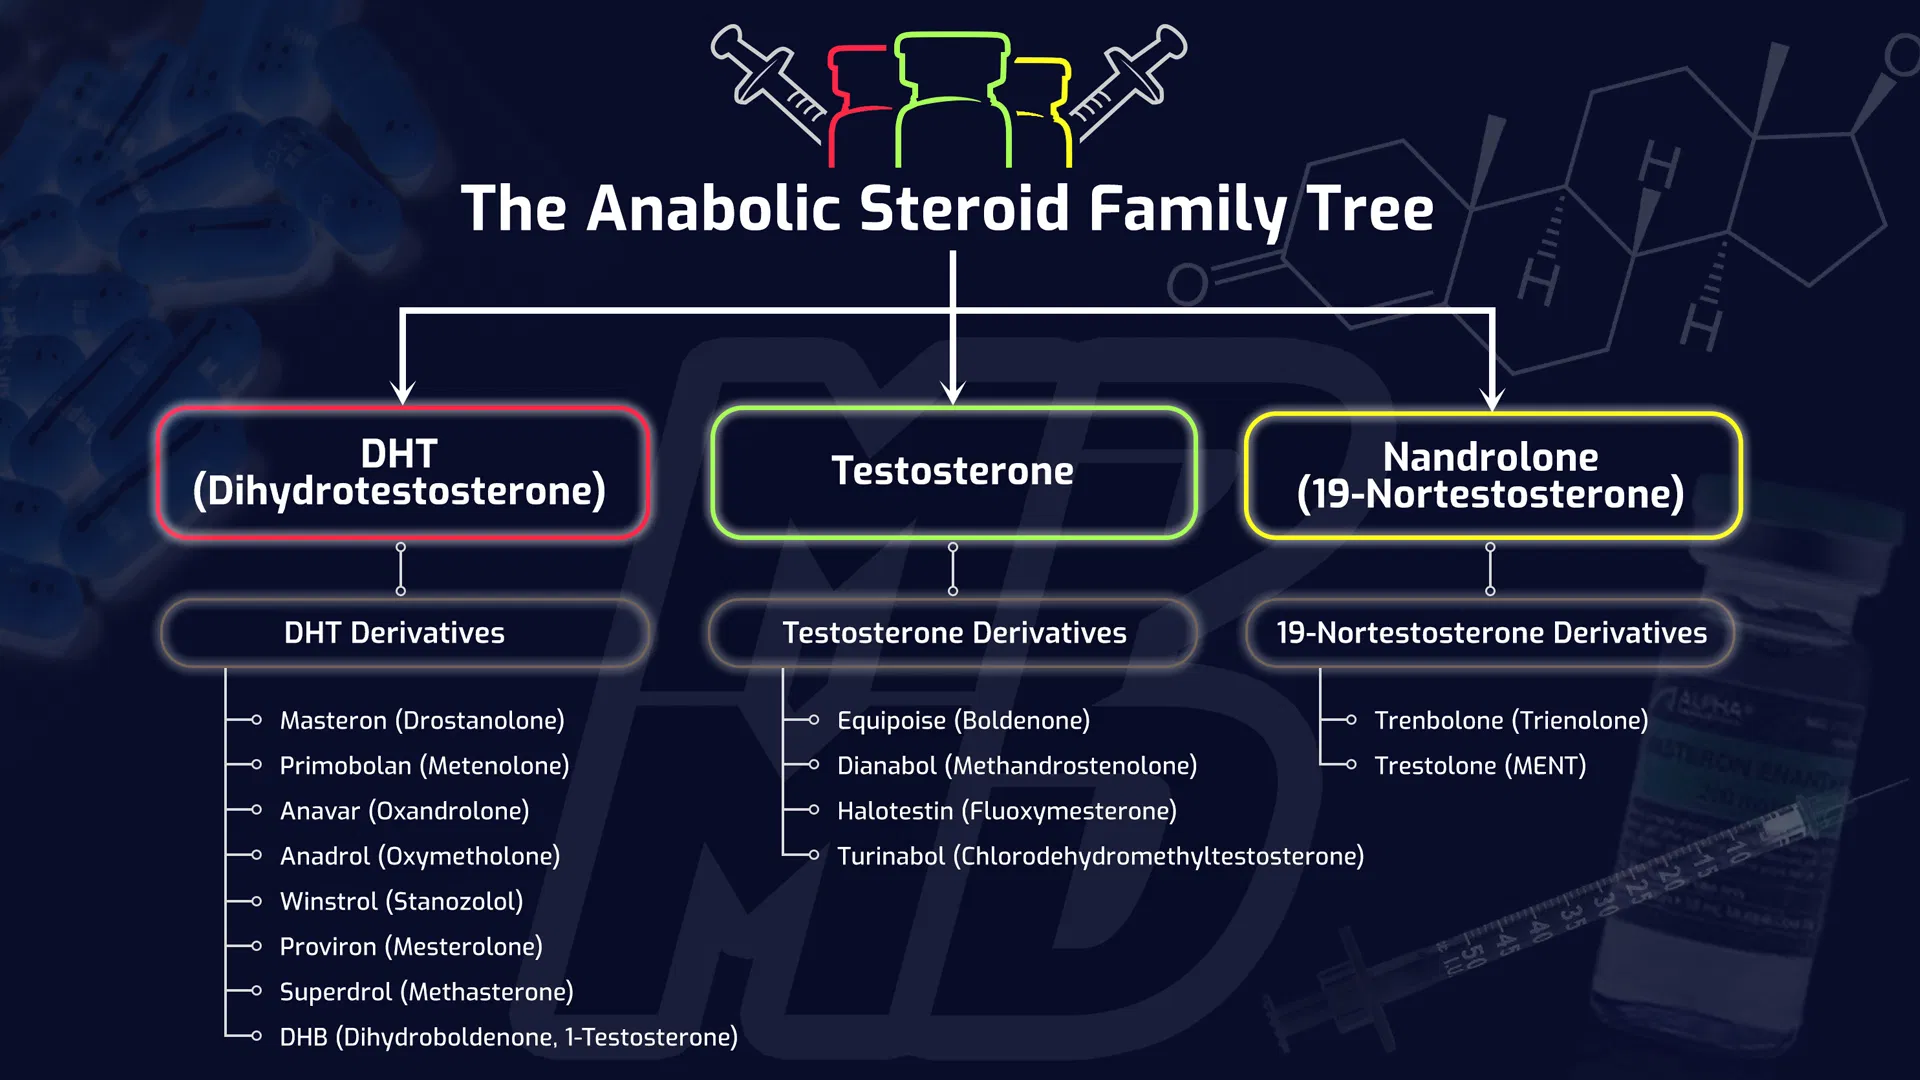
\includegraphics[scale=0.25]{steroids.png}
		\caption{Classification of Anabolic Steroids. Picture taken from moreplatesmoredates.com}
		\label{fig9}
	\end{figure}

	\begin{enumerate}

		\item Testosterone
                  \footnote{\href{https://www.youtube.com/watch?v=SMaLWzRCmSA/}{Greg Doucette on first testosterone cycle}}
                  \footnote{\href{https://www.youtube.com/watch?v=kIkSrgsIDcY/}{Ryan Ankrom on testosterone}}
                  --- this is synthetically made testosterone that comes as an oil in a bottle from which you have to inject multiple times a week. There's 2 main versions of it:
                  cipyonate (depo-testosterone) which is a long ester, meaning you have to inject twice a week, and enanthate which is also a long ester. There is also a third type --- propionate
                  which is a short ester that you have to inject 3 times a week, but it's not as common. People would use around 500mg a week (maybe less, 250 if first cycle), so this means 250mg per
                  injection twice a week. You get all the problems that come with steroids.
                    
		\item Anavar
                  \footnote{\href{https://www.youtube.com/watch?v=J4t4BeQaL8g}{Greg Doucette on Anavar}}
                  \footnote{\href{https://www.youtube.com/watch?v=9A2z7i9yP_4}{Ryan Ankrom on Anavar}}
                  (Oxandrolone is the real name, Anavar is just the brand name) --- oral steroid, one of the safer anabolic steroids out there, less strong than other steroids but really expensive
                  (could be more than \$300 for only one cycle). Part of the DHT family so it speeds up hair loss.
                  It's high on the anabolic scale and low on the androgenic scale (popular among women). One of the most popular steroids out there overall.
                  In theory expect to get results 2 - 10 times faster than being natural. Highly likely to be fake when buying since it's so expensive.
                  It's not aromatized into estrogen, so estrogen levels should stay normal.
                  It has a short half-life so people take it twice a day. Men use around 50mg (25mg x 2) a day and women around 5mg a day.

		\item Trenbolone
                  \footnote{\href{https://www.youtube.com/watch?v=tIvJh53jVfY/}{Greg Doucette on Trenbolone}}
                  (or commonly known as Tren) --- injectable. Probably one of the strongest steroids out there, stronger than pure testosterone (in theory 5 times stronger).
                  Part of the Nandrolone family. It's commonly used in cattle to improve strength.
                  It has really bad side effects: it can screw up cholesterol, bad on kidneys, gives insomnia, hair loss, anger issues, impotence. You can find it in multiple
                  variations such as acetate or enanthate but the most common one is acetate (Tren Ace). Men use around 30mg a day.

		\item Winstrol
                  \footnote{\href{https://www.youtube.com/watch?v=wH0A95aktLo}{Ryan Ankrom on Winstrol}}
                  (Stanozolol) --- oral steroid, derived from DHT as well. Used for cutting down. It messes up cholesterol, increases liver toxicity. Does not convert into estrogen.
                  Men use around 40mg a day (20mg x 2).

		\item Halotestin
                  \footnote{\href{https://www.youtube.com/watch?v=W8Gghg6vvuU}{Ryan Ankrom on Halotestin}}
                  (Halo) --- available both orally or as injection. The oral version is more popular. It's a really strong steroid with strong side-effects. It's commonly known for a great increase in
                  aggression, so people use it for strongmen competitions or before training or fighting. It also helps with strength. As side effects it increases hair loss a lot, it's really hard on the liver
                  and every other side effect of steroids. Men use only 10mg a day.

		\item Masteron (Drostanolone propionate) --- injectable, from DHT, usually used for cutting down.

		\item Deca-Durabolin (Nandrolone Decanoate, commonly known as Deca) --- apparently best bulking steroid, it makes you gain a lot of mass, including water and fat at the same time.

		\item Anadrol (Oxymetholone) --- strongest oral steroid, supposedly stronger than testosterone. It comes with a lot of side effects. Even if it doesn't convert to estrogen, it still
                  makes you gain water \& fat.
                  
		\item Dianabol (Methandrostenolone, Dbol) --- second strongest oral steroid, aromatizes into a stronger estrogen so it needs strong AIs.

	\end{enumerate}

        There's a lot more other anabolic steroids that I won't cover: Equipoise (Boldenone Undecylenate), Proviron (Mesterolone), Turinabol (Tbol), Durabolin (Nandrolone Phenpropionate),
        Tetrahydrogestrinone (THG) etc. Bodybuilders tend to use multiple steroids at the same time while doing a cycle --- this technique is called stacking.
        A stack is all the substances someone takes every day while on cycle. You might see videos with bodybuilders sharing the stack they used before a contest.

        \FloatBarrier
        
        \subsection{Selective Androgen Receptor Modulators (SARMs)}

        SARMs are chemical substances similar to anabolic steroids that will try to keep the anabolic effects of steroids while minimizing the androgenic effects.
        They are relatively new chemicals, invented in the late 1990s, and they are an attempt at making a substance that can get the muscle mass increase without
        any of the androgenic side effects (deep voice, hair loss, facial hair, conversion to estrogen etc).
        Androgen receptors are responsible for many of the male characteristics. Normally they get activated when an androgen such as testosterone
        binds to them. Anabolic steroids are also androgens that will bind to these receptors, that's why they give you androgenic features.
        SARMs are selective androgens that will only bind on receptors responsible for muscle growth, hence why they are called selective. In theory this sounds like a magic pill
        that helps you build muscle with no side effects. However, this is not the case. They are still androgens which will signal your brain to produce less testosterone, which
        leads to impotence. Also, they seem to increase blood \& liver toxicity as well since they are taken by mouth. When doing SARMs people do cycles and PCTs afterwards, similar to steroids.
        Only 4 SARMs have been tested on humans: Ostarine (GTx-024, MK-2866), LGD-4033 (Ligandrol, VK5211)
        GSK2881078, PF-06260414 (with bad side effects, such as headaches, decreased appetite, dizziness, upper respiratory infection, fatigue, and anxiety).
        Since they are new they are legal to sell for research purposes only, that's why there's so many online shops out there selling them. I previously mentioned that a lot of these
        products don't contain what they say they do. I will give a bit of information on a few SARMs below

        \begin{enumerate}
		\item RAD-140 (Testolone)
                  \footnote{\href{https://www.youtube.com/watch?v=RAiR9vwJM7Y/}{Ryan Ankrom on RAD-140}}
                  \footnote{\href{https://www.youtube.com/watch?v=INFn1w18bcc/}{Greg Doucette on multiple SARMs}}
                  --- oral administration. One of the safer SARMs out there but more expensive. It's really strong, close to testosterone in strength. 
                  Men normally use 20mg once a day (half-time of 20h). For PCT people use Tamoxifen or hCG if bigger dose was used.
		\item Ostarine (MK-2866)
                  \footnote{\href{https://www.youtube.com/watch?v=Rl676k-rf\_M/}{Ryan Ankrom on Ostarine}}
                  --- originally designed as Osteoporosis \& muscle wasting treatment. It's less strong than RAD-140, usually good for cutting. It's supposed to help
                  with joint \& tendon problems. Some people mentioned it helps with cholesterol and blood glucose levels. Men use around 15mg once a day (half-life of 24h).
		\item LGD-4033 (Ligandrol, VK5211)
                  \footnote{\href{https://www.youtube.com/watch?v=Ha7gSG0lCGw/}{Ryan Ankrom on LGD-4033}}
                  --- really strong SARM, stronger than RAD-140. It's good for bulking, but does not help with fat loss. It's also less safe (most suppressive SARM, which could lead
                  to impotence) than RAD-140 or Ostarine, but cheaper. Long half-life of 24-36h, men usually take 10mg once a day.
		\item S4 (Andarine)
                  \footnote{\href{https://www.youtube.com/watch?v=1e4jVHNUnn8/}{Ryan Ankrom on S4}}
                  --- less strong than other SARMs, usually good for a dry look \& vascularity. It has vision side effects, you can start seeing a yellow tint.
                  Men usually take between 25 and 50mg a day.
        \end{enumerate}

        Other SARMs I won't cover: S-23, ACP-105, LGD-3303, YK-11.

        \subsection{Other PEDs}

        Human growth hormone (HGH) --- this is a hormone responsible for growth in children. You can buy synthetic HGH that has to be injected (prescription only). 
        It's often stacked with steroids by bodybuilders when doing a cycle.
        This is a really expensive substance, you can pay up to \$5,000 a month for it, and the benefits are not that significant.
        \footnote{\href{https://www.youtube.com/watch?v=5F7m8RHf2ZA/}{Greg Doucette and Iain Valliere on HGH}}
        One of the key benefits of growth hormone is faster recovery, as well as less joint problems.
        It also comes with bad side effects if used in higher doses, such as heart problems and acromegaly (a condition where bones grow too big, causing deformations).
        When sold, people advertise it as an ``anti-aging'' drug, which makes it popular, however none of these claims are actually proven and it's considered one of the
        most overrated PEDs out there
        \footnote{\href{https://www.webmd.com/fitness-exercise/human-growth-hormone-hgh}{HGH on WebMD}}. Another PED that helps with HGH is
        MK-677 (Ibutamoren). This is a growth hormone secretagogue, which means it's not a GH itself, but rather it tells your body to produce more GH. It's usually mistaken
        for a SARM. People who used it
        \footnote{\href{https://www.youtube.com/watch?v=sXNnRQh4grU}{Ryan Ankrom on MK-677}}
        reported increased hunger (which is not ideal for cutting) and skin improvements. Men use around 5mg a day of MK-677.

        Turkesterone
        \footnote{\href{https://www.youtube.com/watch?v=zwlHwlOLW9Q}{VitruvianPhysique on Turkesterone}}
        \footnote{\href{https://www.youtube.com/watch?v=T2QKWjEYZqY}{Greg Doucette on Turkesterone}}
        --- this is an ecdysteroid, a substance found in insects and plants that is similar in structure to testosterone, with similar effects. There's been a few studies about this,
        some suggest it doesn't do anything and others suggest that it might help with muscle growth
        \footnote{\href{https://www.ncbi.nlm.nih.gov/pmc/articles/PMC4447764/}{Ecdysteroids: A novel class of anabolic agents?}}.
        Turkesterone gained a lot of popularity recently since a few famous youtubers started promoting it.
        People who tried it reported that it does work but mostly just helping with strength, a bit similar to creatine but a little more powerful.
        \footnote{\href{https://www.youtube.com/watch?v=zwlHwlOLW9Q}{VitruvianPhysique on Turkesterone}}
        Currently it's really expensive and it might not be worth it for the benefits it gives.

        Fat burners --- I'm first going to talk about over the counter fat burner pills
        \footnote{\href{https://www.amazon.co.uk/Bullets-K-CYTRO-Weight-Management-Supplement/dp/B08N43P8S3/}{Example of fat burner pills on amazon}}.
        Contrary to what the name suggests, these don't actually burn fat but rather suppress appetite. They usually contain a combination of ephedrine, caffeine and
        aspirin (ECA stack
        \footnote{\href{https://www.healthline.com/health/eca-stack}{ECA stack on Healthline}}). I've never tried a fat burner before, but I did notice coffee suppresses hunger for me,
        which is why I find it easier to do something like intermittent fasting where I don't eat anything in the morning and just have coffee.
        There are also substances that actually help burning fat, but these ones are not approved for human consumption. The first example is GW-501516 (Cardarine)
        \footnote{\href{https://www.youtube.com/watch?v=XrNZIO2k06I}{Ryan Ankrom on GW-501516}}
        \footnote{\href{https://www.youtube.com/watch?v=dbBOWljeLiw}{Greg Doucette on GW-501516}}
        which is commonly mistaken for a SARM. It helps a lot with endurance by making cardio super easy.
        It does so by making your body better at burning fat
        rather than glycogen. It should also increase your BMR, making you burn extra calories in a day without doing anything.
        However there was a study about it where it was found to cause cancer in rats, but the doses administered were 50 times the normal dose and for 2 years at a time.
        People use around 20mg a day. Similar substances to GW-501516 are SR-9009 and SR-9011, both with promising results for fat loss.

        Clenbuterol
        \footnote{\href{https://www.webmd.com/pain-management/what-you-need-to-know-about-clenbuterol-for-bodybuilding}{Clenbuterol on WebMD}}
        --- this is also a fat burner that works really well, with serious side-effects such as heart problems and even death.
        Some people claim it's more dangerous than steroids, at least in high doses.
        It works by increasing your body temperature and making thermogenesis burn more calories (so it increases your BMR).
        It also lowers appetite. People take anything between 10 and 120mcg a day. It's often used in combination with T3 (brand name Tiromel),
        which is another substance that increases metabolism in the body. 

        Fragment 176-191
        \footnote{\href{https://www.youtube.com/watch?v=8Hp1ExYShKI}{Greg Doucette on Frag 176-191}}
        \footnote{\href{https://www.youtube.com/watch?v=e4pnPjw2exE}{Ryan Ankrom on Frag 176-191}}
        --- another fat burner, probably the strongest out there. The only downside is that you have to inject it (under the skin).
        It's part of the growth hormone responsible for burning fat. People would use between 300 and 1,000mcg a day, for up to 6 weeks (slowly increase the dose, since
        your body gets used to it), usually right before a contest to get down one extra body fat \%. There's no known serious side-effects.        

        Diuretics
        \footnote{\href{https://www.healthline.com/health/diuretics}{Healthline article on Diuretics}}
        --- these are pills that will make you lose water via urine. They are mostly used for contests to get a leaner look right before the event, since water is stored between skin and muscles. Also
        people use them to make weight for a specific class since you can lose up to 1-2 kg of water with these pills (even outside bodybuilding, in martial arts for example). They come with side-effects
        such as dizziness, muscle cramps and even kidney failure.

        Blood doping
        \footnote{\href{https://www.webmd.com/fitness-exercise/blood-doping}{Blood doping on WebMD}}
        --- this is a technique mostly used by cyclists to be able to perform better in competitions. You can increase oxygen carrying capacity to the muscle ($VO_2max$
        \footnote{\href{https://en.wikipedia.org/wiki/VO2_max}{$VO_2max$ on Wikipedia}}) by increasing the amount of
        hemoglobin in the bloodstream, for example by injecting erythropoietin (EPO). This will improve endurance when exercising.

  \chapter{Workout}

        The skeletal muscles in our body are responsible for every type of movement we do. They contract and relax which makes the skeleton move around. I previously explained that
        a muscle contracts when ATP is released by the mitochondria inside the muscle. For this it needs oxygen, which is carried to the muscle via the blood inside the veins, and
        either carbohydrates (glycogen) or fat. This is a really basic overview of how muscles work. In this chapter I will try to describe the different types of muscles we have,
        how to train them and how to do a workout plan.
  
        \section{Muscle Groups}

        There are more than 600 skeletal muscles in our body
        \footnote{\href{https://en.wikipedia.org/wiki/Skeletal_muscle}{Skeletal muscles on Wikipedia}}. However, when people train to build muscles they only
        focus on only 9 major muscle groups:

        \begin{itemize}
          \item In the arms: biceps, triceps and deltoid (sometimes referred to as the shoulder, although the shoulder is technically the bone in that area).
          \item In the core: abdominal muscles (``abs'' or the more scientific name --- rectus abdominis), pectoral muscles (``pecs'', ``chest'' or pectoralis major) and
            lateral muscles in the back (``lats'' or latissimus dorsi).
          \item In the legs: quadriceps (``quads''), hamstrings and calves (triceps surae).
        \end{itemize}

        Some people or more advanced bodybuilders might also train forearms (arms), traps (trapezius, from back) and glutes (gluteus maximus, the bum, this is more common among women to train)
        \footnote{\href{https://www.youtube.com/watch?v=rKE63BBouP8}{Khan Academy on 11 major muscle groups to train}}
        \footnote{\href{https://www.healthline.com/health/exercise-fitness/muscle-groups-to-workout-together}{Healthline article on major muscle groups}}.
        However, for most men starting out I don't think it's necessary to train these.

	\begin{figure}[h]
		\centering
		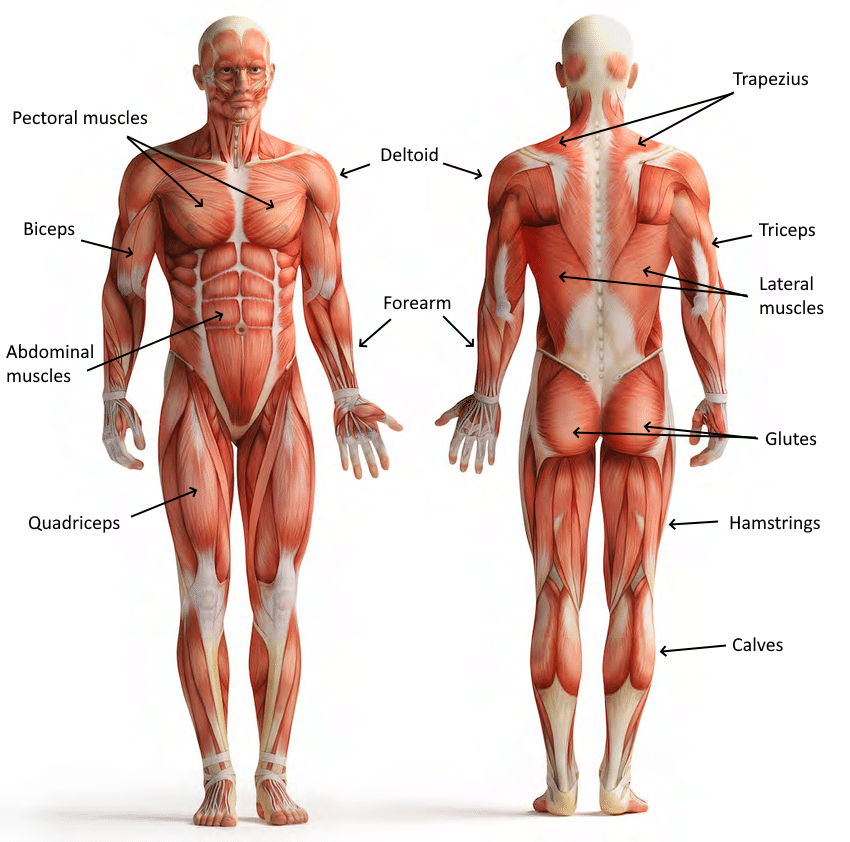
\includegraphics[scale=0.6]{skeletal-muscles.png}
		\caption{Example of 12 major muscle groups people could train in the gym}
		\label{fig10}    %
	\end{figure}

        Each muscle group activates for different type of movement. For example, the pectoral muscles activates when you push something with your arms at chest level (so when your arms are
        perpendicular to your body). In the same push movement you also use the triceps and the frontal part of the deltoid (the deltoid has 3 sections, also called heads --- anterior,
        intermediate and posterior).
        It's interesting how these muscles work, if you push down with your arms
        (and you keep your back straight) the muscles that are mostly responsible for the push are the triceps. As you start to increase the angle your hands make with your body, you get more
        pectoral muscle activation and less triceps. After chest level, the pectoral muscles will start to be less and less engaged while the deltoid will kick in. The push right above your head will
        use mostly deltoid and nothing else. Another type of movement is when you pull something towards you. This will activate both biceps and lateral muscles (back). Normally pulling towards you
        will use more lateral muscles and pulling up (with a supinated grip --- palm facing the body) will use more bicep. The forearm is used in wrist movements, even when just stabilizing the writs
        in a pull exercise.
        Finally for legs, pushing something with your legs will activate most muscles in there and glutes as well. There's also more specific movements that activate muscles more in isolation that I
        will describe in the Exercises section.

        \section{Muscle Growth}

        The muscles in your body are made to adapt to the activities you perform daily. If one day you start lifting weights that feel heavy to you every single day, then over time your body will
        adapt to make these lifts feel easy. This will include muscles bigger in size but also other adaptations (such as neural adaptations for example). It's important to note that in order to
        grow bigger in size you have to push yourself to perform lifts or activities you find difficult, so that your body can adapt and do better next time. When you exert this type of stress on
        your muscles, you will create microtears in the muscle fibers. Your body will then try to repair these tears, making your fibers stronger at the same time. This repair process is called
        muscle protein synthesis (MPS) and is known to take 36h, as previously discussed. This means that for 36h after you trained, you must make sure you have proteins in your body so that
        amino acids from proteins can be added to your muscles. The 36h window is also the reason why some people won't train the same muscle group less than 36h apart (usually take at least
        2 days break between training it again), so that it gets time to properly repair.

        Another thing worth discussing here is muscle soreness. This is commonly referred to as Delayed Onset Muscle Soreness (DOMS)
        \footnote{\href{https://www.webmd.com/fitness-exercise/features/sore-muscles-dont-stop-exercising}{Muscle soreness on WebMD}}
        \footnote{\href{https://www.youtube.com/watch?v=S8PycfGxIxY}{VitruvianPhysique on muscle soreness on Youtube}}
        \footnote{\href{https://www.youtube.com/watch?v=vlGZfIgc6Vk}{Athlean-X on muscle soreness on Youtube}}. You usually get it when you exercise after a long break,
        so it's not due to the microtears in the muscle fibers, which always happen when you exercise. You can experience muscle soreness 8 to 48h after you exercise and it's believed to
        happen because of eccentric contractions (the lengthening part of the exercise, for example when you extend your arm during a bicep curl)
        \footnote{\href{https://www.ncbi.nlm.nih.gov/pmc/articles/PMC2278966/}{Muscle damage from eccentric exercise article}}. During these eccentric contractions fewer
        fibers are used than for concentric contractions (when lifting the dumbbell up in a bicep curl) for the same weight which causes extra damage to the muscle. If this extra damage is
        big enough (so after a long absence), it can result in the muscle fiber's death which will have to be completely replaced by the body and not just repaired. While the muscles rebuilt
        after soreness are stronger, muscle sourness is not needed for muscle growth, microtears are enough to ensure muscle growth.

        One last thing to mention is sleep, which is widely accepted as very important for muscle growth
        \footnote{\href{https://www.youtube.com/watch?v=13y7P8I8rWo}{Mind Pump Show on sleep on Youtube}}
        . While muscle protein synthesis happens both during the day \& night time,
        it does seem to slow down in sleep deprived people
        \footnote{\href{https://www.ncbi.nlm.nih.gov/pmc/articles/PMC7785053/}{Article on sleep deprivation and MPS}}. Lack of sleep also seems to decrease testosterone levels and affect
        the general health of your body (immune system and so on). Not getting enough sleep can also affect your motivation to exercise and how well you perform the exercises,
        and also your ability to stick to your diet. It's usually recommended to sleep between 7 and 9 hours every day, but don't stress too much if every once in a while you get less sleep than that.

        \section{Exercises}

        In this section I will describe multiple exercises, how to perform them and what muscle groups they target.
        If you've never trained before, it's a good idea to have someone experienced with you when you go train, to show you the correct form for the exercise
        and also watch you perform so that he or she can give you feedback. If you don't know such a person, I know some gyms have induction days when they can show you
        different exercises. As a last resort, there are a lot of helpful youtube channels out there showing you the correct technique for a lot of exercises, such as
        Athlean-X, Buff Dudes, Jeff Nippard, ScottHermanFitness etc. Just search on their channels after the exercise name and you should find something.
        I also found ExRx
        \footnote{\href{https://exrx.net/Lists/Directory}{ExRx exercise directory}} and 
        musclewiki.com to be useful. Both of these offer a list of exercises accompanied by short videos with how to perform them.
        What I recommend if you do look at videos first, you should start with really low weights at first, until you feel that you got the form right.
        The reason you should aim to use correct form is mostly to avoid injuries. If you get injured, you might have to wait a few weeks or even months until
        you can train again, so it's really not worth it. However, don't go on the other extreme, trying to get everything perfectly right. As long as you are
        using the correct muscles for the exercise and you feel the muscle ``burn'' you should get in shape. I've seen cases of bodybuilders who don't really care
        about technique and still get in a great shape.
        
        Before diving into the exercises I want to mention that when you're doing a specific exercise, you have to focus on the muscles it should train. For example, if you do bench press
        you should focus on the pectoral muscles and feel them contracting as you do the exercise. Don't try to do the exercise no matter what, using all the muscles in
        your body. This will most likely lead to injury. Instead, try to use a comfortable weight and do the correct form for the exercise.
        Focusing on specific muscles when training is referred to as the mind-muscle connection
        \footnote{\href{https://www.youtube.com/watch?v=Ip25pzb-wdU}{Jeff Nippard on mind-muscle connection}}. The explanations I'm going to give next are just
        brief overviews and you should at least try to watch videos of someone doing the exercise before attempting it.

        \textbf{Bench press}
        \footnote{\href{https://www.youtube.com/watch?v=vthMCtgVtFw}{Athlean-X on how to perform bench press on YouTube}}
        \footnote{\href{https://www.youtube.com/watch?v=gRVjAtPip0Y}{Buff Dudes on how to perform bench press on YouTube}}
        --- one of the most popular exercises out there. This is a compound lift, meaning it hits multiple muscle groups at the same time: pecs, triceps and frontal delts.
        There's multiple variations of this exercise, for the most common one you sit on your back on a flat bench and use a barbell with weights that you bring to your chest level
        and then push up. When performing this exercise first make sure the bar is centered compared to the bench (and not more on the right or left side), then just sit on your back on the bench
        so that your eyes are on the same line as the bar. Grab the bar so that your fingers are touching the rings on the bar and bring it to chest level. Push up, and at the top your hands should be
        perpendicular to the body and you should be able to feel your chest contracting. Lower the bar slowly down to chest level and repeat.
        Do this with the bar alone (it's usually 20kg by itself) first and make sure you get the movement right.
        Where you grab the bar is not super important, the wider your grip is the more chest you engage, and the narrower it is the more triceps you engage. With wide grip you should be able to
        bench more (in strongmen events the only rule is that your finger should still touch the ring on the bar). Start with whatever feels more comfortable to you, as long as your fingers still
        touch the ring on the bar. While performing the exercise you should have your feet stable on the ground, slightly behind your knees 
        to be able to push (and lift your bum up). Your back should also be slightly arched.
        You might see people actually pushing with
        their feet and having an extremely arched back when doing the bench press. This helps with strength, but starting out I don't think it's that important to do.
        Apart from the flat version you can also do it on an incline bench (it hits upper pectoral muscles better) or a decline (lower chest) and also with the dumbbells instead of barbell.
        Using dumbbells will make sure both hands are doing same amount of work during the exercise. You can also find bench press machines in the gym, which also hit the pectoral muscles.
        However, when exercising with a barbell you're also balancing the bar, pushing with both hands at the same speed.
        Starting off with a machine and then
        moving to a bench press you'll find it difficult to balance the bar at first. Another difference is that you also have more freedom without a machine. You might find it difficult
        to adjust the machine to your size so you might get more joint pain from it. Finally, you might feel like using heavier weights on the machine since it's safer than the bench.
        Normally when performing heavy lifts with barbells it's good to have someone that can help you in case you can't push it anymore (this is called a spotter). It's dangerous to lift
        heavy weights without a spotter, people actually died from this.

        \textbf{Overhead press}
        \footnote{\href{https://www.youtube.com/watch?v=2N5P_iWkluQ}{Athlean-X on how to perform overhead press on YouTube}}
        \footnote{\href{https://www.youtube.com/watch?v=F3QY5vMz_6I}{Buff Dudes on how to perform overhead press on YouTube}}
        --- another popular exercise. It's also called the military press or shoulder press with the barbell. In this exercise you push the bar above your head, working the
        deltoid. It's considered a compound exercise, training the core as well. For this exercise you have a rack that can hold the barbell high, close to your neck area. You pick up
        the barbell, put it on your chest under your head. Grip the barbell shoulder width apart. You start by moving your head backwards a little, leaving room for the barbell to go up.
        You push the barbell up and after it's above your head you also slightly push your head forward, so that the bar is above your head, making a straight line with your body. You lower
        the bar down, moving your head back again and placing it on your chest. Repeat the movement. Similar to the bench press, you can also use dumbbells or you can sit down, activating the
        core better. Most gyms will have a shoulder press machine which seems to cause less back problems than the overhead press.

        \textbf{Squat}
        \footnote{\href{https://www.youtube.com/watch?v=q1fCgfieNEs}{Athlean-X on how to perform the squat on YouTube}}
        \footnote{\href{https://www.youtube.com/watch?v=Dy28eq2PjcM}{Buff Dudes on how to perform the squat on YouTube}}
        --- an important compound exercise for legs, it works all muscles in the legs and glutes as well. You start with the barbell on your back (shoulders), with legs shoulder width apart.
        Your feet / knees should point slightly outwards.
        You then have to lower the weight down --- first start with a hip rotation, sticking your bum out a bit. Then lower yourself down as if you were to sit down on a chair, keeping your
        back straight. Stop the movement when the hips are slightly below the knees. Then push up with your legs, keeping your back straight until you are back to starting position. Repeat.

        \textbf{Deadlift}
        \footnote{\href{https://www.youtube.com/watch?v=hCDzSR6bW10}{Athlean-X on how to perform the deadlift on YouTube}}
        \footnote{\href{https://www.youtube.com/watch?v=-4qRntuXBSc}{Buff Dudes on how to perform the deadlift on YouTube}}
        --- another compound exercise for legs \& back. In this exercise you start with the barbell on the ground and all you have to do is lift it up.
        You use your hands only to hold the bar, so it's not an arm exercise. Also, your fingers will need some adjusting too, since the weights are really heavy.
        Place your feet underneath the barbell so that they are sticking on the other side. They should be on the same line with your hips. Grab the bar just outside your legs area. 
        There's different grips you can use, for example the overhand grip (or normal grip --- both hand palms facing towards you).
        If you start lifting really heavy weights with this grip you might start feeling that the
        bar is rolling outside your palms. This is why people use a mixed grip (one hand with the palm facing towards you and the other one outside). If you start using a mixed grip,
        make sure you alternate between which hand is pointing towards you and which outside, to avoid any muscular imbalances.
        First part of the deadlift is a leg press, while you hold the bar, push with your legs up (similar to the squat) keeping your back straight and chest up. When your hands are at knee level
        push forward with your bum, bringing your full body to a straight line. At this point you can either drop the barbell to the ground if you can (if you are in a public gym and it's not too loud
        for example) or lower it slowly back down. There is higher risk of injury when you lower it back down, that's why a lot of bodybuilders will just drop it on the way down.
        Instead of using a straight barbell you can also use a hex bar (or trap bar), which makes the deadlift easier and less prone to injury. There's another variation to the conventional deadlift,
        where you start with the legs further apart than just hip level. This is called a sumo deadlift and it makes it easier for you to lift heavier weights.
        While the deadlift is one of the most famous exercises out there, it's not exactly needed to build a good physique. There's a lot of good leg \& back exercises you can do instead
        of the deadlift. However, the deadlift is the exercise where you can lift the most amount of weight off the ground. Competitive powerlifter can lift more than 3 times their own bodyweight in a
        deadlift.

        \textbf{Pull-ups}
        \footnote{\href{https://www.youtube.com/watch?v=sIvJTfGxdFo}{Athlean-X on how to perform a pull-up on YouTube}}
        \footnote{\href{https://www.youtube.com/watch?v=vw5Xmu5CIew}{Buff Dudes on how to perform a pull-up on YouTube}},
        \textbf{chin-ups} \& \textbf{lat pull-downs}
        --- really famous compound exercise for lateral muscles (back) and biceps. Pull-ups are really common exercises in calisthenics. You have a bar above your head that you grip with your palms facing
        away from your body. The grip should be slightly outside shoulder width (whatever feels comfortable). You then pull yourself up until your neck is above the bar and then lower yourself down and
        repeat. As easy as it sounds, pull-ups are really difficult exercises for beginners since you have to pull your entire bodyweight up and most people starting to train don't have this strength.
        If you can't do a pull-up, what you can do is to start on the pull-down machine or do assisted pull-ups, either on a special machine or using
        a resistance band to help you. The lat pull-down machine is exactly as a pull-up, except you are using a machine and you pull the bar down towards you, with some weight attached to it.
        You grip the bar the same way and this time you bring it down to your chest rather than neck.
        If you've been training for a long time and are in a good shape, you might be able to do too many pull-ups in one go. At this point, it
        becomes more of an endurance exercise than muscle building one. What you can do to lower your repetitions range (more on this later) is to add some weight to your body and do weighted
        pull-ups. Finally a chin-up is the same as a pull-up, except you grip the bar with your palms facing you (supinated grip). This will activate the biceps more and it's actually easier to
        do than a pull-up, so if you are just starting out you might find it easier to start with chin-ups and switch later to pull-ups. Regarding which one should you use, between a chin-up and
        a pull-up, they're actually pretty similar. It really depends what workout plan you follow. I personally do pull-ups but do bicep isolation exercises as well.

        \textbf{Dips}
        \footnote{\href{https://www.youtube.com/watch?v=vi1-BOcj3cQ}{Athlean-X on how to perform a dip on YouTube}}
        \footnote{\href{https://www.youtube.com/watch?v=wjUmnZH528Y}{Buff Dudes on how to perform a dip on YouTube}}
        --- another common exercise in the calisthenics world. This exercise is for triceps and chest. You grab 2 bars on each side of you, pushing yourself up and down.
        If you want more chest activation you bend more towards the front. If you want more tricep activation you keep your back straight. Similar to pull-ups, there are machines to
        help out if you can't perform a bodyweight dip right away (although dips are much easier than pull-ups). You can do a seated dip on the machine, which can be a really good
        tricep exercise if you keep you back straight against the seat. Similarly you can do weighted dips, tying a weight around your waist.

        \textbf{Rowing}
        \footnote{\href{https://www.youtube.com/watch?v=T3N-TO4reLQ}{Athlean-X on how to perform rowing on YouTube}}
        \footnote{\href{https://www.youtube.com/watch?v=h4nkoayPFWw}{Buff Dudes on how to perform the Pendlay Row on YouTube}}
        --- another exercise for the lats and biceps. You sit in a similar position when you start a deadlift, but with much lower weight and you just use your arms to bring the barbell to your body.
        There's a lot of variations of this exercise (such as the Pendlay Row), you can also do it with dumbbells
        \footnote{\href{https://www.youtube.com/watch?v=EEFHHOCfHgw}{Athlean-X on how to perform dumbbell rowing on YouTube}}
        \footnote{\href{https://www.youtube.com/watch?v=1G8czSqCqEA}{VitruvianPhysique on best back exercise on Youtube}}. I personally prefer the seated chest supported row machine
        \footnote{\href{https://www.youtube.com/watch?v=6_xDB8oMkKE}{Greg Doucette on best back exercises on YouTube}}.

        \textbf{Bicep curl}
        \footnote{\href{https://www.youtube.com/watch?v=yTWO2th-RIY}{Athlean-X on how to perform bicep curls on YouTube}}
        --- the first isolation exercise we are going to discuss here. Also, one of the easiest exercises to perform out there. You start with the dumbbell in your hand lowered down, with the palms
        facing away from you, and you just curl it up towards your chest. You then slowly lower it back down and repeat the exercise.
        I just want to mention that in practice it's actually impossible to have true isolation exercises, since there's always several muscles that help
        with every movement. For the bicep curl, you also train forearms a bit, since they are used to stabilize the wrist while you pull up the dumbbell.
        There's multiple variation of the bicep curl, you can do it with dumbbells, barbells or even cables (which I prefer).

        \textbf{Tricep pushdowns}
        \footnote{\href{https://www.youtube.com/watch?v=REWv05om0ho}{Athlean-X on how to perform tricep pushdown on YouTube}}
        \footnote{\href{https://www.youtube.com/watch?v=2-LAMcpzODU}{ScottHermanFitness on how to perform tricep pushdown on YouTube}}
        --- another isolation exercise, this time for the triceps. In this exercise you grab with both hands either a rope or a bar connected via a cable to some weights.
        The bar position is usually around head level and you have to bring it to chest level and then push down only with the
        forearm part of your hand, keeping your elbows locked in place. Body position is slightly bent forward. Start a bit away from the machine and adjust position properly (with low weights)
        until you feel good tricep activation.

        \textbf{Pec fly}
        \footnote{\href{https://www.youtube.com/watch?v=Iwe6AmxVf7o}{ScottHermanFitness on how to perform high cable chest fly on YouTube}}
        \footnote{\href{https://www.youtube.com/watch?v=-EIhKMDSjBY}{Jeff Nippard on pec fly for upper chest on YouTube}}
        --- this is an isolation exercise for the pectoral muscles. There's multiple variations to do it: cables, dumbbells or machines.
        On the cable variation you start with your hands almost parallel to the body but slightly bent and you bring them to a perpendicular position, almost touching (similar to bench press top
        position, but hands are closer together), while contracting the chest as much as you can.

        \textbf{Lateral raises}
        \footnote{\href{https://www.youtube.com/watch?v=3VcKaXpzqRo}{ScottHermanFitness on how to perform dumbbell lateral raises on YouTube}}
        \footnote{\href{https://www.youtube.com/watch?v=q5sNYB1Q6aM}{Athlean-X on how to perform dumbbell lateral raises on YouTube}}
        ---
        isolation exercise for the deltoid. There are multiple variations of this: with a dumbbell or with cables. In the dumbbell version you start with your hand lowered and lift it sideways up.
        This will use the deltoid to pull the weight up. You normally do both hands at the same time.
        In the cable version you might want to have the cable between your legs and pull up again, one hand at a time.

        \textbf{Rear delt machine}
        \footnote{\href{https://www.youtube.com/watch?v=6yMdhi2DVao}{Mind Pump TV on how to use rear delt machine on YouTube}}
        ---
        isolation exercise for the rear (posterior) deltoid muscle. You sit down with your hands pointing forward and you slowly push the bars backward until they are on the same line with your body.
        The same machine is also used for pec fly, but on different settings (make sure you use the pin for the rear delt at the top of the machine).

        \textbf{Leg press machine}
        \footnote{\href{https://www.youtube.com/watch?v=IZxyjW7MPJQ}{ScottHermanFitness on how to use the leg press machine on YouTube}}
        \footnote{\href{https://www.youtube.com/watch?v=Uerf4Mj60Ug}{Mike Thurston on how to use the leg machines in the gym on YouTube}}
        ---
        compound exercise for legs. There's different machines for this one. The most common one you sit down and push horizontally with your legs on some pad. There's another variation where you
        have to load the machine with weights and push almost vertically up against a pad. This exercise hits quads, hamstrings, glutes and calves a bit.

        \textbf{Leg extension machine}
        \footnote{\href{https://www.youtube.com/watch?v=YyvSfVjQeL0}{ScottHermanFitness on how to use the leg extension machine on YouTube}}
        \footnote{\href{https://www.youtube.com/watch?v=YyvSfVjQeL0}{Jeff Nippard on how to do leg extension exercises on YouTube}}
        ---
        isolation exercise for the quads. You sit down on the machine, start with your legs down and extend them up slowly. You might experience some knee shaking at first, but they usually get used
        to the exercise after a while.
        
        \textbf{Leg curls}
        \footnote{\href{https://www.youtube.com/watch?v=ELOCsoDSmrg}{ScottHermanFitness on how to do seated leg curls on YouTube}}
        \footnote{\href{https://www.youtube.com/watch?v=1Tq3QdYUuHs}{ScottHermanFitness on how to do prone leg curls on YouTube}}
        ---
        isolation exercises for the hamstrings (also referred to as the bicep of the leg). This exercise resembles the bicep curl you do for arms, except this time you curl with your legs
        towards your bum.
        There's multiple variations such as the seated leg curl or the prone leg curl.

        \textbf{Calf raises}
        \footnote{\href{https://www.youtube.com/watch?v=YMmgqO8Jo-k}{ScottHermanFitness on how to do standing calf raises on YouTube}}
        \footnote{\href{https://www.youtube.com/watch?v=YMmgqO8Jo-k}{Jeff Nippard on how to train calves on YouTube}}
        \footnote{\href{https://www.youtube.com/watch?v=esdQSIxteQg}{Athlean-X on how to train calves on YouTube}}
        ---
        isolation exercise for calves. Calves are used in a similar way to forearms, they stabilize the ankle. In this exercise you raise your heel up, pushing against some weight to train the calves.
        There's multiple variations \& machines for this exercise.

        Abdominal muscles exercises
        ---
        there's a lot of types of exercises here, I will only describe a few of them. One thing to note is that everyone has abs, but they are usually covered in fat so they will only show if you drop
        in body fat \%. Training your abs will help you get bigger muscles but they will still not show unless you diet down.
        Your abs can't grow that big (like your legs for example) and you can't really train abs for strength, most of the exercises will have high rep count using bodyweight.
        Also, you train abs a bit while doing other exercises such as overhead press. For this reason a lot of bodybuilders won't train abs specifically and still get great abs.
        Personally I think it makes a small difference to train abs as well, so I do train them like other muscle groups.
        Most abs exercises are done on a gym mat on the floor. Using a mat makes it easier for your knees, elbows and back while performing the exercises.
        Probably the most common exercise is the \textbf{sit-up}
        \footnote{\href{https://www.youtube.com/watch?v=1fbU_MkV7NE}{Livestrong.com on how to do sit-ups on YouTube}}, although there's been a debate around that it's bad for your back and
        that crunches are better
        \footnote{\href{https://www.youtube.com/watch?v=y5BpvYGyVb0}{Athlean-X on sit-ups on Youtube}}. For sit-ups you sit on your back on the mat, lift your knees up in a comfortable position.
        You then try to lift yourself up all the way to the knees level by using your abs. Avoid using the arms or back for this. I personally keep my hands on my chest and contract my abs
        while lifting myself up.
        \textbf{Crunches}
        \footnote{\href{https://www.youtube.com/watch?v=Xyd_fa5zoEU}{Livestrong.com on how to do crunches on YouTube}}
        are really similar to sit-ups, but instead of lifting yourself all the way up to knee level, you just do it half-way.
        
        \textbf{Leg raises}
        --- another famous ab exercise, sometimes also referred to as leg lifts. There's a lot of variations for this one, like sitting down on your back on the mat
        \footnote{\href{https://www.youtube.com/watch?v=JB2oyawG9KI}{Livestrong.com on how to do leg raises on YouTube}}, hanging on a bar
        \footnote{\href{https://www.youtube.com/watch?v=Pr1ieGZ5atk}{Athlean-X on how to do hanging leg raises on YouTube}}
        \footnote{\href{https://www.youtube.com/watch?v=hdng3Nm1x_E}{ScottHermanFitness on how to do hanging leg lift on YouTube}}
        which is more difficult, or even holding yourself with your elbows and forearms on a pad in what's called the captain's chair leg raises
        \footnote{\href{https://www.youtube.com/watch?v=ghwdoXHeiIk}{ScottHermanFitness on how to do captain's chair leg raises on YouTube}}
        \footnote{\href{https://www.youtube.com/watch?v=CU2-V80_JsA}{ScottHermanFitness on how to do another version of captain's chair leg raises on YouTube}}.
        In the mat variation, you sit on your back, keep your legs together and slowly raise them to perpendicular level and back down, without touching the ground.
        In the hanging variation you lift either your legs or your knees up, but this time while hanging. You might find it difficult to keep balance, it usually happens when you
        don't control the exercise for the full motion, and you just swing with your legs. Try to start with your legs at a small angle from your body line, and raise your traps a bit
        \footnote{\href{https://www.youtube.com/watch?v=7qPYYw3lPSA}{Athlean-X on how to avoid swinging on hanging leg raises YouTube}} or try using a barbell behind your back
        \footnote{\href{https://www.youtube.com/watch?v=0A4qGKbKMbE}{Mind Pump on how to avoid swinging on hanging leg raises YouTube}}. There's a few other variations of this exercise,
        like the hanging leg rotations
        \footnote{\href{https://www.youtube.com/watch?v=LtSbWD-Z9m8}{Jeff Seid doing leg rotations on YouTube}}
        or hanging leg twists.

        There's so many ab exercises you can perform on the mat
        \footnote{\href{https://www.youtube.com/watch?v=Sqo29SsJqpA}{Mike Thurston on ab workout on YouTube}}
        \footnote{\href{https://www.youtube.com/watch?v=zzD80vCLq0Y}{Athlean-x on ab workout on YouTube}}. Some examples: \textbf{bicycle}
        \footnote{\href{https://www.youtube.com/watch?v=9FGilxCbdz8}{Livestrong.com on how to do the bicycle on YouTube}}, \textbf{reverse crunches}
        \footnote{\href{https://www.youtube.com/watch?v=hyv14e2QDq0}{Livestrong.com on how to do reverse crunches on YouTube}}, \textbf{heel touches}, \textbf{knee crossovers},
        \textbf{russian twists}
        \footnote{\href{https://www.youtube.com/watch?v=drvh39387LY}{Livestrong.com on how to do ab twists on YouTube}}
        and many more.
        I won't describe each into details, feel free to watch the videos I linked and search for more online and try each to see which work best for you. Another good option is to attend an
        ab workout class (most gyms offer these) and see how you like those exercises as well. I'm going to list again all exercises described in this section, categorized by muscle group
        just to have a good overview in Figure \ref{fig11}
        
	\begin{figure}[h]
		\centering
		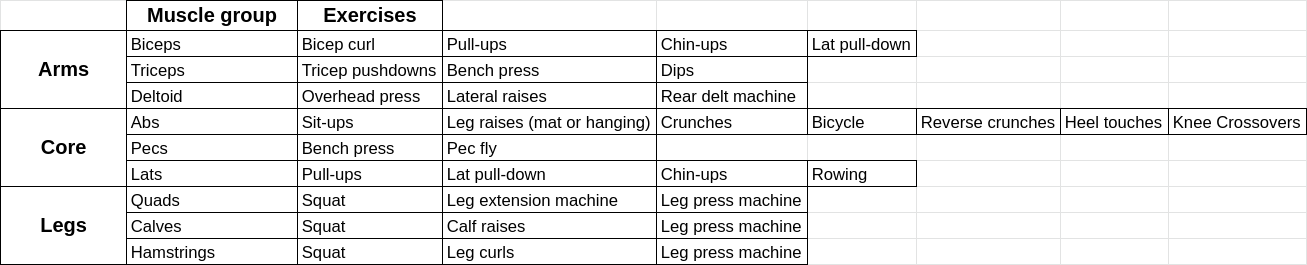
\includegraphics[scale=0.4]{exercises.png}
		\caption{Overview of all the exercises discussed, by muscle group}
		\label{fig11}
	\end{figure}

        \section{Workout Plan, Splits}

        In the previous section I discussed about different exercises you can do for each muscle group. A full movement for one exercise is called a rep (repetition). For example, for the bench press
        exercise if you push the bar up and down 12 times, you've done 12 reps. At some point you have to stop, either because you can't do another rep (training to failure --- happens because your
        muscle runs out of ATP) or because you just want to stop, still having reps in the tank. When you stop you've just finished a set. A workout plan, at its basics represents the 
        the number of reps in a set, the number of sets for each exercise, the weight being used and a bunch of others factors like intensity, frequency, volume, rest between sets that we will discuss
        next. There is no perfect workout plan out there, just like for dieting, here opinions are really different on how you should train --- how often, how many sets, how many reps etc.
        I will try to highlight what's known to work but at the end of the day you still have to try different workout plans and see what works best for you and what gives you the best results.

        First, let's look at the number of reps in a set. The most common idea out there is that you should do a different number of reps based on your goal: maximum increase in strength, muscle size or
        endurance. Yes, strength and muscle size are not the same thing, although they are directly correlated, I will talk more about this later. For strength training, you should do 5 reps or less
        for each exercise, as heavy as you possibly can. I do think it's important to train to failure here, you should adjust the weight such that your 5th rep is almost a failure.
        For maximum muscle growth, also known as muscle hypertrophy, 10-12 reps is considered optimal. Finally, for endurance you should aim to do as many reps as possible with a lower weight.
        Training to failure is also known as workout intensity. Should you train to failure for muscle growth? There are different opinions about this, some say training to failure is not optimal
        while others say it is, but they all seem to agree that starting out you shouldn't train to failure
        \footnote{\href{https://www.youtube.com/watch?v=39YvjFRiGac}{Greg Doucette on intensity vs volume and training to failure}}.
        
        It also matters how you perform each rep, if you have a slow controlled movement or if you are fast or explosive. For muscle hypertrophy people usually recommend a slow movement.
        The time it takes you to finish a set is called time under tension
        \footnote{\href{https://www.healthline.com/health/exercise-fitness/time-under-tension}{Time under tension on healthline}}
        (your muscle being under the tension from the weight) or TUT for short. Most people recommend a TUT of 40-60 seconds for optimal muscle hypertrophy, although there are studies contradicting this
        \footnote{\href{https://www.t-nation.com/training/the-new-science-of-time-under-tension/}{Article on ideal TUT on T-nation}}. If we follow the 40-60 seconds rule, and you do 10-12 reps then
        each rep should take you 4 to 5 seconds (usually 1 second for the concentric movement and 3 seconds for the eccentric one). For strength people usually recommend 4 to 20 seconds of TUT.

        Between sets you have to rest, to allow your muscles to build more ATP. The optimal rest time is also different based on your goal. For muscle hypertrophy people recommend a rest time of
        30 to 90 seconds so up to almost 2 minutes, for strength 2 to 5 minutes and for endurance it's only 20 to 60 seconds
        \footnote{\href{https://www.healthline.com/health/fitness/rest-between-sets}{Rest time on healthline}}. Honestly I wouldn't stress too much about rest time, just try
        not to do one set after the other too fast since you are not doing cardio with the weights, and also don't wait way too long between sets since your muscles are warmed up and ready to go.

        Next, let's look at how many sets you should do. This is commonly referred to as workout volume (either per workout or per week). A common rule is that starting out you should aim for
        5 to 10 sets per week for each muscle group
        \footnote{\href{https://www.youtube.com/watch?v=HTJTpVwg2Oo}{VitruvianPhysique on training volume on Youtube}}
        . For example you can do 3 sets of bench press, twice a week to reach 6 sets and it should be enough for training pecs. As you train for longer, you
        should increase the volume (increasing weight and volume over time is referred to as progressive overload) up to 20 sets a week for a muscle group, for experienced lifters (more than 5 years of
        lifting). For example, you can do 4 sets of bench press, 4 sets of pec flys twice a week, which lands you at 16 sets for pecs per week. Add 4 sets of incline press and you should be good.

        Finally, let's look at frequency
        \footnote{\href{https://www.youtube.com/watch?v=5NqtfvR7v4A}{VitruvianPhysique on training frequency on Youtube}}
        \footnote{\href{https://www.youtube.com/watch?v=PrUgmKRbOxE}{Greg Doucette on training frequency on Youtube}}
        \footnote{\href{https://www.youtube.com/watch?v=eTxO5ZMxcsc}{Jeff Nippard on training frequency on Youtube}}
        , or how often you should train one muscle group per week. There are theories out there that after you trained a muscle group, you should wait for the 36h of
        MPS to end before training it again, so that the muscle fibers are completely repaired. In this theory, after the 36h have passed, the muscle is just resting, so to optimally
        build muscles you should train the same muscle group 2-3 days apart. This is one of the most popular workout routine out there: train each muscle group twice a week.
        There are also theories out there that waiting for MPS to finish doesn't matter, and that frequency is key to building both muscles and strength. In this case you should train muscle groups as
        often as possible, even every day, multiple times a day
        \footnote{\href{https://www.t-nation.com/workouts/bulgarian-training-simplified/}{Article on Bulgarian method on T-nation}}
        . However, if you do 8 sets every day for every muscle group you might be overdoing with the volume, so low workout
        volume is key here (e.g. 2-3 sets for each muscle group per day, which gives 14 to 21 sets if you train every day).

        Just reiterating over all the workout factors described here
        \begin{enumerate}
		\item TUT \& number of reps --- how long your set will take. For example, you could aim for 10-12 reps with a TUT of 40 seconds
		\item Intensity --- how close you are to failure at the end of a set. For example you could stop when you almost fail a rep
		\item Volume --- how many sets for a particular muscle group you do in a week. For example, you can aim for 10-20 sets in a week, based on your experience
		\item Frequency --- how often do you train one muscle group in a week. For example, you could train one muscle group twice a week
		\item Rest between sets --- how much you wait between sets. For example, you can wait 30 to 90 seconds
        \end{enumerate}

        There's a few other things that are worth discussing. First, the weight you use for your sets. You normally adjust this so that you hit your rep count or TUT, being really close to failure.
        However, if you do one set after the other you might not be able to do the same reps with the same weight on your 2nd or 3rd set. In this case you might want to lower it. This is similar to
        a dropset
        \footnote{\href{https://www.healthline.com/nutrition/what-is-a-drop-set}{Dropsets on Healthline}}
        where you always train to failure with a small rest time, always lowering the weight. Others might recommend ramping sets
        \footnote{\href{https://www.t-nation.com/training/thibaudeau-on-ramping/}{Ramping sets on T-nation}}
        , which are the opposite --- you start with a lower weight and you keep increasing it, doing fewer and fewer reps with each set. There is also a technique where you increase the weight and then
        decrease it back --- pyramid sets
        \footnote{\href{https://www.menshealth.com/fitness/a36317637/pyramid-sets/}{Pyramid sets on Men's Health}} which some people recommend for building strength. There's even a technique
        where you keep changing the weight and reps in a set every day --- daily undulating periodization
        \footnote{\href{https://pubmed.ncbi.nlm.nih.gov/11991778/}{Article on DUP}} (DUP). Personally I wouldn't stress too
        much which technique you end up using, just pick something you feel comfortable with. However, before you start doing your sets for a particular exercise, you have to start with a warm-up set
        (except for abs where you don't lift any weight).
        This is a set with a really low weight for roughly 20 reps. For example for bench press you could start with the bar alone (20kg) and do 20 reps to warm up the muscles. This will help you avoid
        injury, especially when you start doing heavier weights because the muscle is not ready to lift heavy, it needs some warming up. Another thing you might want to do is stretching before or
        after exercise. Some people say this helps with recovery, but I personally never do it and I've never had any issues. Something else that people claim it helps with recovery is an ice bath,
        although this doesn't have any scientific support
        \footnote{\href{https://www.ncbi.nlm.nih.gov/pmc/articles/PMC2938508/}{Article on post exercise ice water immersion}}

        The plan with what you train each day is referred to as splits
        \footnote{\href{https://www.youtube.com/watch?v=RDWyqnGhmWY}{Athlean-X on workout splits on YouTube}} (for example on Monday you train biceps, on Tuesday you train pecs etc).
        The first split I'm going to discuss is the full body split. In this split
        you train your full body in a single workout, multiple times a week. Starting out this might be ok, but as you get more and more experienced and you need to do more sets and more types of
        exercises, doing a full body workout will take you hours and hours. Arnold Schwarzenegger was known to do full body workouts 3 times a week, but most of us don't have 5h every day to train, so
        a full body workout split becomes impossible.

        Push, pull, legs --- probably the most famous split out there. This combines muscles used for the same movements together, and allows you to let them rest before having the same
        workout routine again. This workout plan would look something like this: on Monday you do a push day --- pecs, triceps and shoulders (bench press, overhead press, dips, tricep pushdowns etc).
        On Tuesday you have a pull day --- lats \& biceps (pull-ups, pull-downs, bicep curls etc) and finally on Wednesday you have a legs day (squat, leg curls, leg extensions etc). A lot of people
        train abs on the same day as legs, so it becomes a legs \& abs day. The following days --- Thursday, Friday \& Saturday you just repeat the same days from Monday to Wednesday and this is the
        entire workout plan. To avoid working out on the weekends, some people try to do an upper \& lower body split for Thursday \& Friday, so basically legs (and maybe abs) on Friday and everything
        else on Thursday. 

        I just briefly want to mention the bro split, a split that I've seen used as an example of a bad split. In this split you sometimes only train one muscle group in a day, and other times you
        have ``arms'' for a day (which I assume it's biceps, triceps and shoulders) followed by chest, which hits triceps again on the bench press. From the examples I've seen it looks like a really
        inconsistent split, without trying to hit each muscle group the same number of times per week, and with low frequency.
        
        You are free to create a workout plan however you like. If all of this sounds too complicated, a good idea is to start with a popular workout plan and adjust to your needs. For example, start
        with a push, pull, legs \& abs split, train only the 9 major muscle groups I mentioned in the Muscle Groups section, hit each twice a week with a total of 6 sets of 10-12 reps
        (aim for 40 seconds of TUT) and a resting time of 30-90s. If you do
        everything right (nutrition as well), this should give you good results. As you keep training, every now and then you might want to try a new exercise or change any of the workout factors:
        volume, intensity, TUT, reps or frequency. Try to see what works best for you.
        I put a workout plan example below
        \footnote{\href{https://docs.google.com/spreadsheets/d/10_J9RkAH8QSpqSg65c3OfkovorFkVoU3Bl213Y9xWUo/edit}{Workout Plan Example on Google Spreadsheets}}
        , feel
        free to access it from the link and copy the spreadsheet to your own account and update with your own exercises and weights. Adjust the weight so that you hit the 10-12 reps range.
        Increase weight over time if it's becoming too easy with the same weight. After training for a while (after you see the progress slowing down, could be 1 year of training)
        you should add more sets to the same exercises, increase the weight and also add additional exercises as you can see in Figure \ref{fig13}
        \footnote{\href{https://docs.google.com/spreadsheets/d/1A1-G2KrdD_O9NgyKty6OGyuEq619M2QIW6Ple3kbSSI/edit}{Advanced Workout Plan Example on Google Spreadsheets}}.

	\begin{figure}[h]
		\centering
		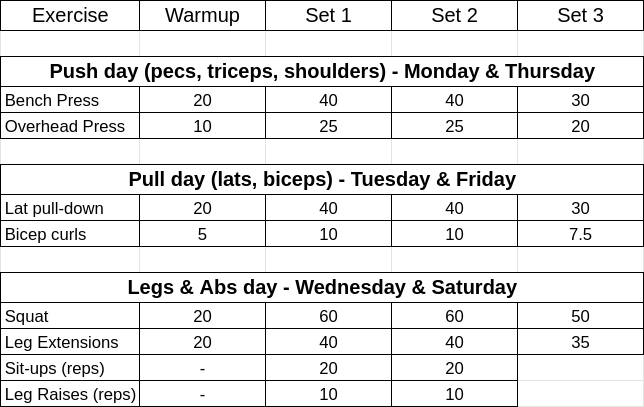
\includegraphics[scale=0.5]{workout-plan-1.png}
		\caption{Example of a workout plan you can start with. The weights are all in kg and just random examples, you need to see what weights you can use instead}
		\label{fig12}
	\end{figure}

	\begin{figure}[h]
		\centering
		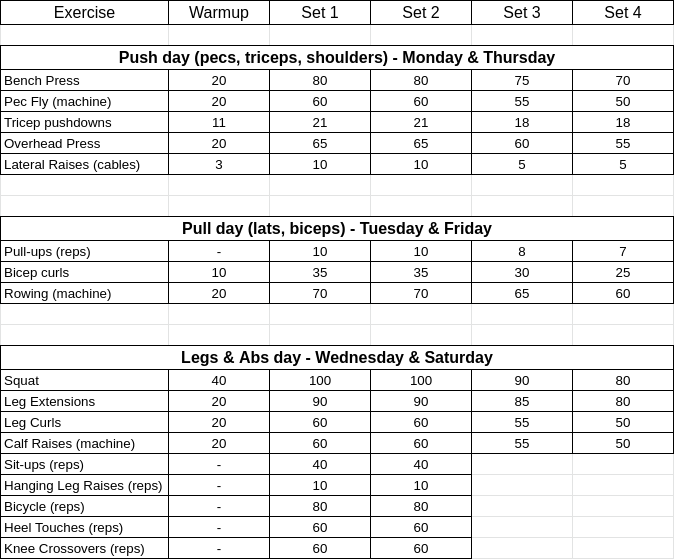
\includegraphics[scale=0.5]{workout-plan-2.png}
		\caption{Example of a workout plan after training for some time. The weights are all in kg and just random examples, you need to see what weights you can use instead}
		\label{fig13}
	\end{figure}

        \section{How Much Should You Lift}

        In the previous section I talked about training for different goals such as strength or muscle hypertrophy, and adjusting the weight to hit the desired TUT \& intensity.
        With this in mind, the weight you lift doesn't matter, for example if you train for hypertrophy just adjust the weight so that after 12 reps you either fail or are as close
        as possible to failure. This implies you're using slow movements and correct form as well. There's a lot of strength standards on the internet
        \footnote{\href{https://www.youtube.com/watch?v=LrDJXIQ_-eg}{Jeff Nippard's strength standards on Youtube}}
        \footnote{\href{https://www.t-nation.com/training/strength-standards-are-you-strong/}{Strength standards on T-nation}} that will give you numbers you should aim to lift based
        on your bodyweight and experience for bench press, squat and deadlift. I think it's interesting to be aware of these, just so you have something to compare to, but I wouldn't give
        them too much importance, unless you want to become a powerlifter. Powerlifters are strength competitors that will try to lift as heavy as possible for squat, bench press \& deadlift.
        They are divided by weight class, so maximizing lift weight to bodyweight ratio is important. To give an example, Taylor Atwood
        \footnote{\href{https://barbend.com/taylor-atwood-3-american-records-2021-usapl-nationals/}{Article on Taylor Atwood}}
        at 74kg was able to bench press 195kg (2.6x his bodyweight), squat 303kg (4x) and deadlift 340.5kg (4.6x). These are really impressive numbers, most lifters are happy
        if they reach 1.25x, 1.5x and 2x ratios for the 3 lifts. If you weight 70kg then a goal you can set is to bench 87.5kg, squat 105kg and deadlift 140kg.
        Most people will be able to squat more than they can bench press, and deadlift more than they can squat. However, this is heavily influenced by genetics and some might be able to
        squat more than they can deadlift. The progress you make on strength levels is also much faster if you train for strength rather than hypertrophy, but more on this later. I'm
        illustrating below an example of strength levels based on bodyweight and experience, but keep in mind that if you do want to compete in powerlifting, you will have to do better
        than elite.

        \begin{figure}[h]
		\centering
		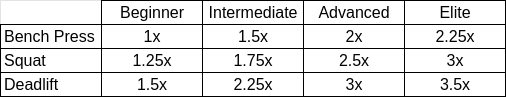
\includegraphics[scale=0.65]{strength-standard-1.png}
		\caption{Jeff Nippard’s strength standard you could follow for powerlifting. Each value is the ratio of the lift compared to bodyweight}
		\label{fig14}
	\end{figure}
        
        \section{Muscular Potential}

        Something everyone agrees on is that building muscles slows down over time. If you manage to put on 5kg of muscles in your first year of training then in your second year you'll only
        manage to put on half of that, and so on until after 10 or more years you'll reach a plateau, barely putting any muscle size on in a year. This is what people call reaching your genetic
        potential or limit. This is of course, without taking any PEDs. How much muscle you can put on each year is highly debatable, and different people say different things, but they all
        agree that your genetics
        \footnote{\href{https://www.youtube.com/watch?v=KC4Sc_XgmZ0}{VitruvianPhysique on good genetics on Youtube}}
        highly influence this value, and that gaining muscle slows down at a nearly inverse exponential rate, every year being able to gain about half the mass of the previous year.
        Some people would say that with good genetics you can put up to 5.5kg of muscle in your first year of training
        \footnote{\href{https://www.youtube.com/watch?v=r4Hyli_4frY}{Greg Doucette on muscular potential on Youtube}}. In this model you should expect to gain at most 20kg of muscle after you reached
        your genetic potential, after 10+ years of training. Others say you could expect up to 11kg
        \footnote{\href{https://www.youtube.com/watch?v=vQ2vxH4eOGw}{ScottHermanFitness on Muscular Potential on Youtube}} of muscle gains in your first year, which would result in up to 27kg in 10 years.
        Finally, some people claim you can gain up to 1.5\% of your lean bodyweight every month (Alan Aragon model). In any case, most people agree that it's super rare to gain more than 1kg of muscle mass
        in a month. You might think that's slow, but 10kg of muscle mass makes a huge visual difference. For most people that just want to be fit, 10kg of muscle is enough to reach their fitness goal.

        \begin{figure}[h]
		\centering
		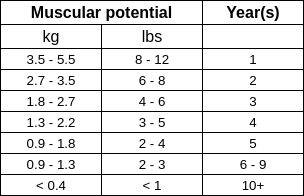
\includegraphics[scale=0.65]{muscular-potential-1.png}
		\caption{Greg Doucette’s muscular potential model for good genetics}
		\label{fig15}
	\end{figure}

        \begin{figure}[h]
		\centering
		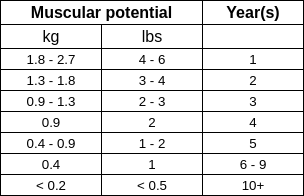
\includegraphics[scale=0.65]{muscular-potential-2.png}
		\caption{Greg Doucette’s muscular potential model for bad genetics}
		\label{fig16}
	\end{figure}

        \begin{figure}[h]
		\centering
		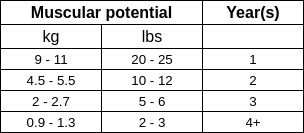
\includegraphics[scale=0.65]{muscular-potential-3.png}
		\caption{Lyle McDonald's muscular potential model}
		\label{fig17}
	\end{figure}

        \begin{figure}[h!]
		\centering
		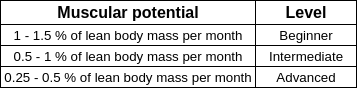
\includegraphics[scale=0.65]{muscular-potential-4.png}
		\caption{Alan Aragon's muscular potential model}
		\label{fig18}
	\end{figure}
        
        There's also theories out there that the amount of muscle you can gain is based on your body type ---
        mesomorph, endomorph or ectomorph (also known as somatotypes)
        \footnote{\href{https://en.wikipedia.org/wiki/Somatotype_and_constitutional_psychology}{Somatotypes on Wikipedia}}. The ectomorph type struggles to gain weight, either fat or muscle.
        The endomorph is the opposite type, where you can put both fat and muscle really fast, and finally the mesomorphs get the best of both worlds, being able to put on muscle really fast
        but not fat. There's no scientific support for this somatotype classification, it comes from a psychologist who also said that your body type affects your personality, which makes it
        really hard to believe. Personally I wouldn't give it too much importance. Those who support this classification also say there is a spectrum for each type, so you belong to all types
        with a value between 1 and 7 for each, so you're not only endomorph and that's it. Another interesting theory is that your muscle potential is dictated by the size of your wrist
        \footnote{\href{https://www.youtube.com/watch?v=xLrNHB5O6f8}{Athlean-x on muscle potential myths on Youtube}}. Again, not a really scientific theory, so I wouldn't give it importance.

        \section{Muscle Size vs Strength}

        I previously mentioned that muscle size and strength are not the same thing. There are powerlifters out there who can lift more than bodybuilders who are heavier and more muscular
        than them. As a random example, Jonnie Candito was able to bench 157.5kg at 83kg
        \footnote{\href{https://www.ipfwatch.com/lifters/jonnie-candito/)}{Jonnie Candito on ipfwatch.com}}, more than Brandon Harding in 2018
        \footnote{\href{https://www.youtube.com/watch?v=UVxsfzE1pag)}{Brandon Harding benching 156kg on Youtube}} benching 156kg at which I assume to be over 90kg. Search online for pictures with both of
        them to see the difference in muscle size.
        One explanation for why strength is not the same as muscle size is that strength is also given by neural adaptations
        \footnote{\href{https://pubmed.ncbi.nlm.nih.gov/3057313/)}{Neural adaptation to resistance training article}}, that is the ability of your nervous system to activate your muscles. This
        neural adaptation is believed to increase a lot when you just started training and slow down over time. It's also believed that women have faster neural adaptations than men, allowing them
        to get stronger faster than men, in the first few months of training. So basically stronger people have better neural adaptations.
        Other potential explanation for why strength is not just muscle size is that your muscle is made of different types of fibers, like type 1, type 2a or type 2x
        \footnote{\href{https://www.youtube.com/watch?v=eU-fFi0D8Es)}{VitruvianPhysique on strength vs size on Youtube}}. Type 2a can generate more force than type 1, so stronger people probably
        have more of type 2a than type 1. This is just a hypothesis though.
        One final potential explanation is that muscle size is given by both sarcoplasm and myofibrils, and stronger people have more myofibrils while bigger guys have
        more sarcoplasm. The bottom line is that your body will adjust to what you throw at it --- if you always push for heavier lifts, even for 1 rep (usually referred to as 1 rep max or 1RM) then it
        will adjust to become stronger. Using less weight with less intensity and higher volume will have better hypertrophy results
        \footnote{\href{https://www.healthline.com/health/exercise-fitness/hypertrophy-vs-strength)}{Healthline article on hypertrophy vs strength}}. There is also something to say about technique,
        changing your technique might allow you to lift heavier. Powerlifters spend a lot of time on improving their technique (the arched back when bench pressing etc).

        \section{Fixing Muscle Asymmetry, Lagging Body Parts}

        After training for a while you might notice muscle asymmetry in your body, for example your left bicep might be bigger than your right bicep. There's a lot of reasons why this happens, and it's
        really common as well. First of all, the human body is not perfectly symmetrical, even on the face the right side is not identical to the left side. The same is true for muscles, and it's
        mostly due to genetics --- you might have more muscle fibers in one side, store less fat so that it appears bigger or even poorer mind muscle connection.
        Using a bad form when doing the exercises could also be a root issue.
        The only way to fix a bad form is to either have someone with you that can watch you exercise or just record yourself and watch afterwards. A lot of the times you might be the only one who notices
        these muscle asymmetries, and they are not that important anyway. Look at Jay Cutler's biceps, who won Mr. Olympia multiple times, there is a clear size difference between them.

        If you really want
        to fix muscle asymmetries in your body then there's a few things you can do, but remember that a perfect symmetrical body is not possible
        \footnote{\href{https://www.youtube.com/watch?v=zQTmfOsSXN0}{Jeff Nippard on fixing muscle asymmetries on Youtube}}
        \footnote{\href{https://www.youtube.com/watch?v=rlOa9L1gOA8}{Greg Doucette on fixing muscle asymmetries on Youtube}}

        \begin{itemize}
          \item Do more volume on the side that is smaller, for example one extra set per workout
          \item Do more reps on the side that is smaller, for example one extra rep with each set you're doing
          \item Try to improve the mind muscle connection for the weaker side either by focusing more on that muscle when performing the exercise or do a ``pre-activation'' set for the weaker side
            before a compound lift. A ``pre-activation'' set is an isolation warmup set, maybe using an increased TUT while trying to focus as much as possible on contracting the muscle
        \end{itemize}

        Dumbbells are probably one of the best tools to fix these asymmetries, since you can perform an exercise with only one side at a time. For example, if your right bicep is smaller than
        the left one, you can do one extra set of bicep curls with the right hand.
        You might also want to do less bilateral exercises (like pull-ups) that might create asymmetry in the first place, and also do asymmetry training until the smaller side is bigger than the other
        side, allowing for the stronger side to catch up at some point, when you start training normally again
        \footnote{\href{https://www.youtube.com/watch?v=FP2dyni-dgA}{Renaissance Periodization on fixing muscle asymmetry on Youtube}}.
        Just a note, really big side differences, if they are not due to genetics, will tend to fix themselves without any changes to your training program, as long as exercise form is correct.
        The weaker muscle will have to work harder to keep up with the stronger one, which means more intensity that will result in more growth, especially considering the muscle growth has an
        inverse exponential rate. At some point the difference will be unnoticeable, unless the problem is different (mind-muscle connection, genetics).

        Fixing lagging body parts is pretty similar and requires a specialized workout plan. It usually involves more volume for the lagging body part and prioritization in the workout. This means that
        you should start your workout with an isolation exercise for the lagging body part, and have more sets for it overall in a week.
        You might have to slow down overall progress for your entire body, to allow the lagging body part to catch up. Sometimes it might be impossible to have good proportions due to genetics. For example
        Derek from More Plates More Dates has unfortunate chest genetics.

        \section{Getting a Pump, Vascularity}

        I previously mentioned that the muscle needs oxygen for ATP production to be able to contract. Oxygen is carried to the muscle through veins via the bloodstream.
        When you work out, more blood is supplied to the muscle and less to vital organs such as the brain. This explains why you might feel dizzy after an intense workout,
        since your brain is running low on oxygen. The way your body controls blood flow is via vasodilation and vasoconstriction. When a muscle needs more blood,
        the veins supplying that muscle with blood will dilate (vasodilation), allowing for a greater volume of blood to be pumped to the muscle. This is why your veins might
        appear bigger after a workout. On the contrary, to limit the blood supply to a body part, the veins will narrow (vasoconstriction).
        A lot of the blood pumped to a muscle during a workout will get trapped inside the muscle, making it inflate, just like a sponge. This is referred to as ``getting a pump''.
        After getting a pump, the muscle group will significantly grow in size. To be able to notice this on your body, you have to train for at least a few months to put on some size.
        A lot of bodybuilders will take photos of themselves after getting a pump, to appear bigger in size. The same happens during a bodybuilding competition, when competitors will get a pump
        backstage before stepping on stage.

        Vascularity means having a lot of big, visible veins (or superficial veins, the ones on the surface of the body, because there are also deep veins far from the surface) all over your body.
        Because a lot of bodybuilders have good vascularity, this is usually associated with being muscular. However, you might have big muscles and still not be able to see many veins. This usually
        happens because your body fat \% is too high. Superficial veins are sitting on top of muscles, between fat and skin. The more fat you have, the harder it is to see your veins.
        Another reason you might get poor vascularity is of course, genetics. Some people are born with worse vascularity than others. However, vascularity will usually improve with training
        because your body does create more veins to be able to supply more blood to bigger muscles --- process called angiogenesis
        \footnote{\href{https://www.youtube.com/watch?v=N1oCJiw8oTY}{VitruvianPhysique on vascularity on Youtube}}. Bigger muscles will also push veins against the skin, making them appear bigger.
        There are supplements out there that help with blood flow, the most popular one being L-citrulline (sold as citrulline malate). Most of the time you will find citrulline in pre-workout
        powders (as a fun fact, citrulline is naturally found in watermelon), but personally I don't think it makes a big difference to your workout. Bodybuilders might take it before a show
        to help with vascularity, although the effects of it are really small, most of the vascularity comes from low body fat \% and big muscles.
        There's a lot of other factors that affect vascularity, just to name a few:
        water, salt, sugar, temperature (a warm environment is better for vascularity than a cold one, since your blood needs to stay warm), body position (lifting your hand up will give you worse
        vascularity than pointing it down, since blood flow has to fight gravity to go up) etc. However, none of these factors will come close to having low body fat \%.

  \chapter{Fitness World}

  By now you should have a basic understanding of how to make a nutrition \& workout plan, and how to manage your expectations based on your goals. In this chapter I will try to
  list what you can do outside of this book, either to learn more, be part of a community or keep up to date with news from the fitness world. I personally think it's super important
  to be part of a community no matter what you do, it helps tremendously with motivation and how good you feel along the way. If you liked this book and want to get in touch with me,
  you can drop me a message on my instagram \textit{@mihaildu\_fitness}
  \footnote{\href{https://www.instagram.com/mihaildu_fitness/}{Link to my instagram account}}, or join a slack group I created for like-minded people
  \footnote{\href{https://join.slack.com/t/fitness-world-group/shared_invite/zt-1bhw1fakw-X5vr_m1DwEv2tAelIcWj1w}{Slack invite for Fitness World group}}.

  	\section{News}

        Youtube is a good website to stay up to date with news from the fitness world. Nick's Strength and Power
        \footnote{\href{https://www.youtube.com/c/NicksStrengthandPower/videos}{Nick's Strength and Power on Youtube}} is a channel that covers many bodybuilding events, strongman competitions and
        other general fitness events as well. VitruvianPhysique
        \footnote{\href{https://www.youtube.com/user/VitruvianPhysique}{VitruvianPhysique on Youtube}} has a lot of really well explained videos about different fitness concepts. Every now
        and then he might talk about some new article or supplement. Greg Doucette
        \footnote{\href{https://www.youtube.com/user/gregdoucette/videos}{Greg Doucette on Youtube}} has a lot of good information videos, although him screaming at the camera might be
        off-putting for some. These days most of his videos are reaction videos to other fitness youtubers. More Plates More Dates
        \footnote{\href{https://www.youtube.com/c/MorePlatesMoreDates/videos}{More Plates More Dates on Youtube}} does similar videos to Greg Doucette, covering news from Youtube or
        Reddit. Mind Pump Show
        \footnote{\href{https://www.youtube.com/c/MindPumpShow/videos}{Mind Pump Show on Youtube}} is a channel with podcasts where they talk about different topics, all fitness related.
        RenaissancePeriodization
        \footnote{\href{https://www.youtube.com/c/RenaissancePeriodization/videos}{RenaissancePeriodization on Youtube}} has a lot of useful information videos, not really news but since we
        are at Youtube channels I thought I should mention it. Athlean-X
        \footnote{\href{https://www.youtube.com/c/athleanx/featured}{Athlean-X on Youtube}} --- one of the most famous fitness Youtube channels, it has a lot of useful tips on how to perform
        exercises. 
        There's a lot more fitness youtube channels out there that I previously mentioned in this book (Jeff Nippard
        \footnote{\href{https://www.youtube.com/c/JeffNippard}{Jeff Nippard on Youtube}}, Buff Dudes
        \footnote{\href{https://www.youtube.com/c/BuffDudesOfficial}{Buff Dudes on Youtube}}, ScottHermanFitness
        \footnote{\href{https://www.youtube.com/c/scottherman}{ScottHermanFitness on Youtube}}, Mike Thurston
        \footnote{\href{https://www.youtube.com/c/MikeThurston}{Mike Thurston on Youtube}} etc), I won't cover all of them. Just find the ones you enjoy the most.

        Strongerbyscience
        \footnote{\href{https://www.strongerbyscience.com/}{Strongerbyscience website}} --- this is a website with good news on research (Research Spotlight section) and podcasts as well.
        Ergo Log
        \footnote{\href{https://www.ergo-log.com/}{Ergo Log website}} is another website where they list new articles about supplements and PEDs.
        For more general interesting articles you can check T-nation
        \footnote{\href{https://www.t-nation.com/}{T-nation website}}. You might also consider getting an examine.com membership
        \footnote{\href{https://examine.com/store/membership/}{Examine.com membership}} that will give you summaries of studies done each month on nutrition and supplements.
        
        \section{Communities}

        Reddit is usually a good place to find communities about anything. For fitness there is r/Fitness
        \footnote{\href{https://www.reddit.com/r/Fitness/}{Fitness subreddit}}
        and r/bodybuilding
        \footnote{\href{https://www.reddit.com/r/bodybuilding/}{Bodybuilding subreddit}}. If you've never used reddit before, it's a website with groups (subreddits) where people make
        posts that get upvoted or downvoted, with the ability to only see most upvoted posts. There's a lot of fitness subreddits, but r/Fitness and r/bodybuilding seem to be the most
        popular ones. There was a website back in the day called Fitocracy
        \footnote{\href{https://www.fitocracy.com/}{Fitocracy website}} which was using gamification for fitness. This basically means turning fitness into a game where you get points for
        doing the right things, which will allow you to level up. It also had a nice community going on, although it's looking different today. Bodybuilding.com forum
        \footnote{\href{https://forum.bodybuilding.com/index.php}{Bodybuilding.com forum}} is the oldest community for fitness, I've never personally tried it but it might be worth checking.
        There is also the T-nation forum
        \footnote{\href{https://forums.t-nation.com/}{T-nation forum}}, which looks similar. I hope over time my slack group (which I mentioned at the beginning of this chapter) 
        becomes more active, but for now it's just been created so it needs more time to grow.
        
        \section{Resources}

        When it comes down to fitness, there's plenty of books to choose from. The ones I've seen recommended the most are written by Mark Rippetoe --- Starting Strength: Basic Barbell Training
        \footnote{\href{https://www.amazon.co.uk/Starting-Strength-Basic-Barbell-Training/dp/0982522738}{Starting Strength on Amazon}} \& Practical Programming for Strength Training
        \footnote{\href{https://www.amazon.co.uk/Practical-Programming-Strength-Training-Rippetoe/dp/0982522754}{Practical Programming for Strength Training on Amazon}}. These books are focused on
        strength training more than hypertrophy. If you want something more bodybuilding focused then you can try either The New Encyclopedia of Modern Bodybuilding
        \footnote{\href{https://www.amazon.co.uk/New-Encyclopedia-Modern-Bodybuilding-Updated/dp/0684857219/}{The New Encyclopedia of Modern Bodybuilding on Amazon}} by Arnold Schwarzenegger or
        Joe Weider's Ultimate Bodybuilding: The Master Blaster's Principles of Training and Nutrition
        \footnote{\href{https://www.amazon.co.uk/Joe-Weiders-Ultimate-Bodybuilding-Weider/dp/0809247151/}{Ultimate Bodybuilding on Amazon}}. These books go in-depth with training and nutrition, and
        might be too advanced if you don't want to compete in bodybuilding.
        If you are interested more in the science of exercise and what happens to the body when you exercise then you could give these
        books a try: Exercise Physiology: Theory and Application to Fitness and Performance
        \footnote{\href{https://www.amazon.co.uk/Exercise-Physiology-Application-Fitness-Performance/dp/0078022533}{Exercise Physiology: Theory and Application to Fitness and Performance on Amazon}}
        \& Exercise Physiology: Nutrition, Energy, and Human Performance
        \footnote{\href{https://www.amazon.co.uk/Exercise-Physiology-Nutrition-Performance-International/dp/1451193831}{Exercise Physiology: Nutrition, Energy, and Human Performance on Amazon}}.
        A few other books worth mentioning --- Overcoming Gravity
        \footnote{\href{https://www.amazon.co.uk/Overcoming-Gravity-Systematic-Gymnastics-Bodyweight/dp/0990873854}{Overcoming Gravity on Amazon}} which focuses mostly on bodyweight exercises, and
        Anabolics 11th Edition
        \footnote{\href{https://www.amazon.co.uk/ANABOLICS-11th-William-Llewellyn/dp/0999062107}{Anabolics 11th Edition on Amazon}} which goes more in-depth about PEDs.

        There's also plenty of websites with good fitness information, such as Healthline
        \footnote{\href{https://www.healthline.com}{Healthline website}} and WebMD
        \footnote{\href{https://www.webmd.com/}{WebMD website}}. ExRx
        \footnote{\href{https://exrx.net/}{ExRx website}} is good for reference, it has information on nutrition and exercises. You can find really good information on nutrition and supplements
        on examine.com
        \footnote{\href{https://examine.com/}{Examine.com website}}, just input something in the search bar. Finally, some people have recommended Simple Science Fitness
        \footnote{\href{https://ss.fitness/}{Simple Science Fitness website}}, which seems to have introductory information on nutrition and workout.

        \section{Bodybuilding Competitions}

        Taking part in a competition can be a great motivation to stay on track with your progress! However, for most competitions you have to train for at least a few years to be able to do well.
        Competitions are held by bodybuilding organizations and they have multiple divisions in which you can compete. One of the most known organization is the National Physique Committee
        \footnote{\href{https://npcnewsonline.com/}{NPC website}} (NPC). They have 3 divisions for men: Men's Physique, Men's Classic Physique and Bodybuilding, each with their own subdivisions
        based on weight or height. The bodybuilding division cares more about size than looks, while men's physique is more about aesthetics (body shape, symmetry etc). Classic physique is somewhere
        in the middle between the two. If you are interested in participating, take a look over the rules page
        \footnote{\href{https://npcnewsonline.com/official-bodybuilding-rules/}{NPC rules}}. While the contests shown there are only for United States, they do have international contests
        as well, for this check NPC Worldwide
        \footnote{\href{https://www.ifbbpro.com/category/all-categories/pro-qualifier/}{NPC Worldwide}}. They also have a pro league --- IFBB Pro League
        \footnote{\href{https://www.ifbbpro.com/}{IFBB Pro website}}. I am not sure why it's called IFBB, since International Federation of BodyBuilding and Fitness
        \footnote{\href{https://ifbb.com/}{IFBB website}} (IFBB) is a different organization based in Europe, with their own contests. The IFBB from Europe has its own elite pro league,
        IFBB Elite Pro
        \footnote{\href{https://eliteprocard.com/}{IFBB Elite Pro}} which makes it all the more confusing. Anyway, to take part in IFBB Pro League contests you need a pro card (you might've seen
        people claiming they are IFBB Pro athletes, meaning they got their card). To win a card you need to win in a National Championship from NPC against all other weight classes for your division.
        NPC will also host special events, such as Joe Weider's Olympia
        \footnote{\href{https://mrolympia.com/}{Olympia website}}, which is considered the biggest event in bodybuilding. You qualify for the Olympia if you win an IFBB Pro qualifier competition.
        You also get points for finishing 2nd, 3rd etc at these competitions. The top 3 competitors by points will also qualify, as well as the top 5 at a previous Olympia (although the rules
        might change based on circumstances). Olympia has the following divisions for men: Mr. Olympia, 212 Olympia, Classic Physique and Men's Physique. The biggest competitors in the sport take
        part in Mr. Olympia division, where the winner takes home roughly \$500,000, the biggest prize money in bodybuilding. All of the competitors you see at Mr. Olympia are taking PEDs, such
        as anabolic steroids.

        Another big event that is worth mentioning is the Arnold Sports Festival
        \footnote{\href{https://en.wikipedia.org/wiki/Arnold_Sports_Festival/}{Arnold Sports Festival on Wikipedia}} which is a weekend long event hosting bodybuilding, strongman and other fitness
        related competitions. It's usually referred to as the Arnold Classic. The event originated in United States but it's now taking place in multiple locations, such as Spain (Arnold Classic
        Europe), England (Arnold Classic UK), Brazil (Arnold Classic South America) etc. Apart from NPC \& IFBB there's a lot of other organizations hosting bodybuilding competitions, just to name
        a few: National Amateur Body-Builders' Association (NABBA)
        \footnote{\href{https://www.nabba.co.uk/}{NABBA website}}, World Beauty Fitness and Fashion (WBFF)
        \footnote{\href{https://wbffshows.com/}{WBFF website}}, International Competition Network (ICN)
        \footnote{\href{https://www.theedge.com.au/icn-nsw/}{ICN website}} etc. There's a lot more in every country, just look for bodybuilding contest in your area. You could also ask at your local
        gym if they know of any competitions coming up. You might also consider hiring a personal trainer to help you prepare for the competition, and also advise you what division is best for you.

        \subsection{Peak Week}

        The week before a bodybuilding competition is called a ``peak week''. The idea is to make yourself look as muscular as possible within a week,
        by using a few tricks that only work short term. This involves water and carbs manipulations, getting a fake tan and so on. You have to be at a low body fat \% for this to work.
        This technique is also good if you want to do a photoshoot or for whatever reason you want to make yourself look more muscular in a short amount of time. Every bodybuilder has his own peak week
        plan, however they all have a lot of similarities. I did a peak week myself, even though I've never competed, by combining information from VitruvianPhysique
        \footnote{\href{https://www.youtube.com/watch?v=oa2LLw-_I0U}{VitruvianPhysique's peak week}} and Greg Doucette
        \footnote{\href{https://www.youtube.com/watch?v=gCrZF_MMovs}{Greg Doucette's peak week}}. A lot of the peak week plans are not exactly scientific and hard to evaluate each step at how much
        it helps you, but people still do them. This is what I did (starting 4 days before the show/photoshoot)
        
        \begin{itemize}
          \item Day 1 \& day 2: I removed all carbs from my diet, while still hitting my caloric intake (just eat more fat and proteins). This diet is the keto diet. The reason you do this is to
            get rid of all glycogen in muscles. While starting this diet all of a sudden, you might feel really tired and have trouble sleeping. I recommend having something to help with melatonin
            production for sleep (like 5HTP capsules) and maybe pre-workout before training. I trained like I normally do.
          \item Day 3: same as previous 2 days except I removed sodium as well (had less than 2g) and drank a lot of water. Drinking a lot of water should help your body get used to eliminate it
            frequently so that when you stop drinking water the next day, you become as dehydrated as possible. You want to be dehydrated to avoid having too much water between skin and
            muscle. Just keep in mind that drinking a lot of water is dangerous too, since you can
            become overhydrated and potentially die.
          \item Day 4: time to carb up! I ate a lot of junk food, chocolate bars, candy, crisps etc. My sodium intake went back to normal but I barely drank any water.
            I tried to keep my caloric intake normal as well. Again, this day is dangerous
            since you will feel very dehydrated and dizzy all the time. The reason you carb up now is to increase glycogen back inside the muscle. Because you've been depleted for 2 days,
            your muscles should absorb more glycogen then normal, making the overall muscles look bigger.
          \item Day 5: last day (show day), same as day 4, I kept eating junk food and had almost no water. I was trying to aim for 50g of carbs every 2-3h.
            Avoid slow digesting meals, such as those high in proteins or fat to avoid having a big
            stomach. This day I also shaved my upper body and applied a fake tan with a spray (I used the spray that seems to be recommended by most bodybuilders --- Pro Tan
            \footnote{\href{https://www.amazon.co.uk/gp/product/B001F6VDGI/}{Pro Tan spray on Amazon}}) although you might want to use it multiple days in a row, starting day 3 for example.
            Shaving and having a tan will make you appear a lot more muscular. Finally, before my photo shoot I slightly increased my water intake, took about 8g of citrulline mallate and got a pump,
            training every muscle group with low weights and high rep count.
        \end{itemize}

  \chapter{Full Example}

  
  In this chapter I will give a list of steps you could try following to get in shape if you've never trained before, without any extra explanations.
  For full explanations read the previous chapters. Feel free to try what I describe here,
  although some of the steps are more important than others and you might really want to customize this list for yourself. I will try to give examples with each step.
        
        \begin{enumerate}
                \item Buy a bunch of stuff: gym membership, gym clothes, supplements (creatine, multivitamins, whey \& casein protein powder, omega 3 pills). The supplements are not exactly important
                  and could be skipped.
                \item Find your maintenance calories. Use a TDEE calculator like tdeecalculator.net. Example: 2,000 calories a day.
                \item Add 20\% to the value you got in the TDEE calculator. This is your goal every day for the next 3 months of lean bulk. Example: 2,400 calories.
                \item Weight yourself. Take your weight (in kg), multiply it by 2.2. This is the amount of grams of proteins you should aim to eat every day. Example: at 70kg, 154g of proteins.
                \item Decide how you want to hit your daily goals: by cooking in advance (meal prep), by tracking (e.g. using myfitnesspal, paper etc) or a mixture of both. I recommend cooking in
                  advance. To help with your meal plan you can use the meal plan calculator spreadsheet I linked in the nutrition chapter, tracking calories section. Add your favourite ingredients,
                  dishes etc, and play with the values until you hit your daily goal for calories and proteins. You can look at Figure \ref{fig4} for an example of a meal plan.
                \item Create a workout plan. Feel free to use the workout plan example spreadsheet I linked in the workout chapter, workout plan section. In time you will customize this to
                  the exercises you enjoy most, and the weights that are best for you. For how to perform the exercises read the exercises section from the same chapter. For example, do the same
                  exercises from Figure \ref{fig13}, adjust the weights such that you are close to failure after 10-12 reps.
                \item Start your lean bulk for roughly 3 months (4 weeks x 3). Decide on a start date and plan 4 weeks of diet and exercise, followed by 2 days of break from diet and exercise.
                  Make sure you can focus on both nutrition and workout during the 4 weeks, without breaks. 
                  Fill in the weights you are using in the workout spreadsheet. You should notice yourself becoming stronger. Increase the weight (also in the spreadsheet, it's
                  a good way to track it and not forget how much you can lift) to stay in the same rep ranges you are using. After your first 4 weeks and few days of break,
                  repeat the same process 2 more times.
                \item Start your lean cut phase: this phase you will do until you reach a body fat \% you are happy with (it could be 3 months, 6 months... a year). Prepare in advance a spreadsheet
                  where you will log your weight every day. You can use the Weight Log Template from bulking \& cutting section.
                  Compute your TDEE again (your weight should have changed, but more importantly your body fat \%, if you can
                  compute this), this time subtract 20\%. For protein intake aim
                  for more than 2.2x your bodyweight (so maybe 2.5x). Create new meal plan. While you cut down, the weights you can lift should stay at the same value. Do this whole cutting phase in
                  increments of 4 weeks at a time. Have a cheat weekend after each phase, if you really want to. Monitor your weekly average weights, they should be decreasing at a rate between
                  0.45kg and 0.9kg. If the rate is slower, adjust the goal for caloric intake (and meal plan) to be lower.
                  Keep adjusting it until you reach a good rate (adjust every 2 weeks, to give your body time to adapt to changes).
                  Take pictures every few weeks, look at the progress for extra motivation!
                \item After you reached your body fat \% goal it's really up to you what you want to do next. If you want to keep growing in size, go back to a lean bulk. Every time you feel like
                  you put too much fat, go back to a lean cut. Doing a lean bulk shouldn't really put that much fat though. If you just want to maintain your physique try to aim for your TDEE, but you
                  still have to exercise. However, I would decrease the volume a bit. Try to adjust values until you get the results you want, there is no perfect way to compute in advance what you need.
                \item Optional: take supplements both during your bulk \& cut. You can take multivitamins, creatine and omega 3 pills whenever. Whey protein in the morning, casein before bed. I wouldn't
                  take omega 3 if I already have something like salmon in my diet. Same for whey or casein, I wouldn't take powders if I eat something else that has them, at the same times.
                \item Optional: find a workout buddy! This will help you a lot to stay motivated and on track with your goals.
        \end{enumerate}

        That's pretty much it! If you followed this book and got in shape, please do get in touch. I'm more than happy to hear success stories :)

\end{document}
